%\documentclass{article}
\documentclass[final]{pittetd}
\usepackage[square,numbers,sort&compress]{natbib}
\usepackage{graphicx}
\usepackage{amsmath}
\usepackage{url}
\usepackage{subfigure}
\usepackage{float}
\usepackage{calc}
\usepackage{color}
\usepackage{algorithmic}
\usepackage{algorithm}
\usepackage{afterpage}
\renewcommand{\algorithmicrequire}{\textbf{Input:}}
\renewcommand{\algorithmicensure}{\textbf{Output:}}
%% Define a new 'leo' style for the package that will use a smaller font.
\makeatletter
\def\url@leostyle{%
  \@ifundefined{selectfont}{\def\UrlFont{\sf}}{\def\UrlFont{\small\ttfamily}}}
\makeatother
%% Now actually use the newly defined style.
\urlstyle{leo}

\makeatletter  %% this is crucial
 \renewcommand\subsubsection{\@startsection{subsubsection}%
    {3}{\z@}{-1\@singleline\@plus -1ex \@minus -.2ex}%
    {.5\@singleline \@plus .2ex}%
    {\@withperiod\@withgobble\normalfont\expandafter\bfseries}}
\makeatother   %% this is crucial 


\title[]{Software Update Management in Wireless Sensor Networks}
\author{Weijia Li}
\degree{B.S., Nanjing University, 1999}
%\date{July 20th 1967}%             This date is the date of the thesis defense. Default is \today
%\year{1967}                        pittetd will use the current year unless otherwise indicated. So this command is not
%                                   necessary.
\keywords{compiler optimization, code generation, wireless sensor networks, software update}
\subject{Weijia Li PhD thesis}%             
\school{Department of Computer Science}%  


%\includeonly{compiler}

\begin{document}

\maketitle
\committeemember{Dr. Youtao Zhang, Department of Computer Science}
\committeemember{Dr. Daniel Moss\'{e}, Department of Computer Science}
\committeemember{Dr. Bruce Childers, Department of Computer Science}
\committeemember{Dr. Daqing He, School of Information Sciences and Intelligent System Program}
\school{Computer Science Department}
\makecommittee
%
%
%
%%\copyrightpage                     Uncomment this to get a copyright page.
%
%
\begin{abstract}
Wireless sensor networks (WSNs), composed of a large number of low-cost, battery-powered sensors, and a relatively powerful sink node, have recently emerged as promising computing platforms for many non-traditional applications. 

Although the code running on the sensors is preloaded to them before deployment, it may still need updates for many reasons. 
In single application wireless sensor networks (SA-WSNs), sensors need to upgrade the software in order for the WSN to adapt to the changing demands of the users.
In multiple application wireless sensor networks (MA-WSNs), each sensor may have to switch between different applications upon request. Due to the memory size limitation, the sensors may not be able to store the complete image of all the applications in the local memory. 
Thus, the sensors may have to convert a temporarily unwanted application to the wanted application by applying software updates.

Despite the fact that the sensors need such code updates for various reasons, the code update patches are often transmitted via wireless channels, because the sensors are usually left unattended after deployment. As the code is transmitted via battery-powered wireless communication, the energy consumed in the software update can be significant, especially when it happens frequently.

The goal of this research is to design a software update management framework, which
optimizes the energy consumption in WSN software updates. The proposed framework
includes an update-conscious compiler, a patch script generator, and a code dissemination
protocol. First, it generates the new binary image using the update-conscious compilation
techniques, and then compares the new binary with the old binary to generate the patch.
The update-conscious techniques make the new binary code more similar as the old version,
so that the size of the patch script can be reduced. The patch generator summaries high
level binary differences in a script. This technique furthermore reduces the script size.
Finally, the framework transmits the generated patch over the network using an efficient code
dissemination protocol. This technique reduces the time and energy spent in propagating
the update patches over the network. After the sensor nodes receive the complete patch,
they will regenerate the target executable.

This research solves an important problem in WSN study. The designed software update framework will benefit all the WSN users by making the software update procedure faster and more energy efficient. Besides that, it is also the very first research of update-conscious compilation techniques. The motivation of similar code generation in compilation research is another great contribution of this research. 
\end{abstract}
%
\tableofcontents
%\listoftables                      Pittetd will complain if you tell it to create a list of tables when there are no
%                                   tables (as in this sample file). Uncomment this command if you have tables.
%\listoffigures                     Obvious analogous for figures.
%\preface
% This is the text of the preface, with acknowledgments, dedication, etc. It is optional, and you create, as shown, by 
% just saying \preface and starting the preface's actual text. Note that 'foreword' is no longer acceptable as title
% for this preliminary.
%
%Conventions, such as notation (nomenclature) and abbreviations, don't receive their own preliminary page. They can be included as an appendix, or as part of the introduction.
%

\chapter{Introduction}\label{chap:intro}


Wireless sensor networks (WSNs) have recently emerged as a promising computing platform for many nontraditional applications, such as monitoring for wildfires, monitoring oceanic life, and battlefield surveillance. A WSN usually consists of hundreds of sensor nodes that are equipped with the sensors to measure the physical phenomena, such as temperature, humidity, pressure, or movement of objects. Sensing results are constructed into data packets and routed back to sink nodes, which are typically more powerful, user accessible and have fewer energy constraints.

\begin{figure}[h]
\centering
\mbox{\subfigure[Mica2 sensor]{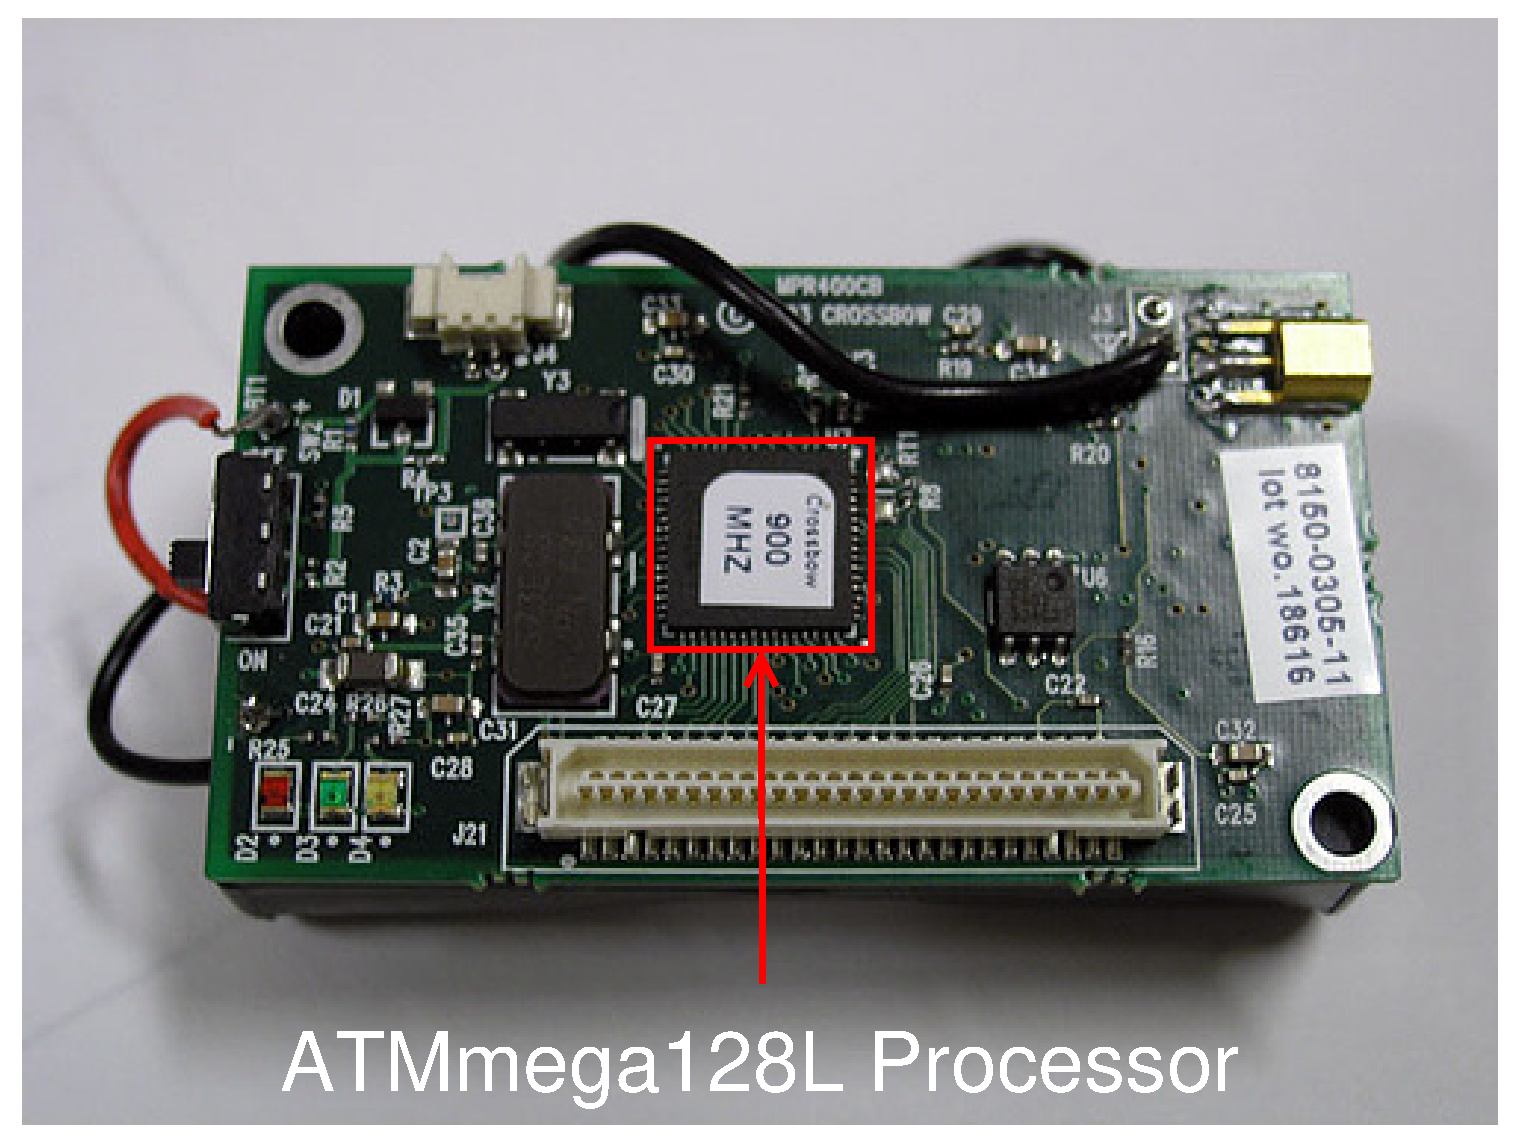
\includegraphics[width=2.6in]{figures/mica2.eps}}
\subfigure[Mica2 block diagram]{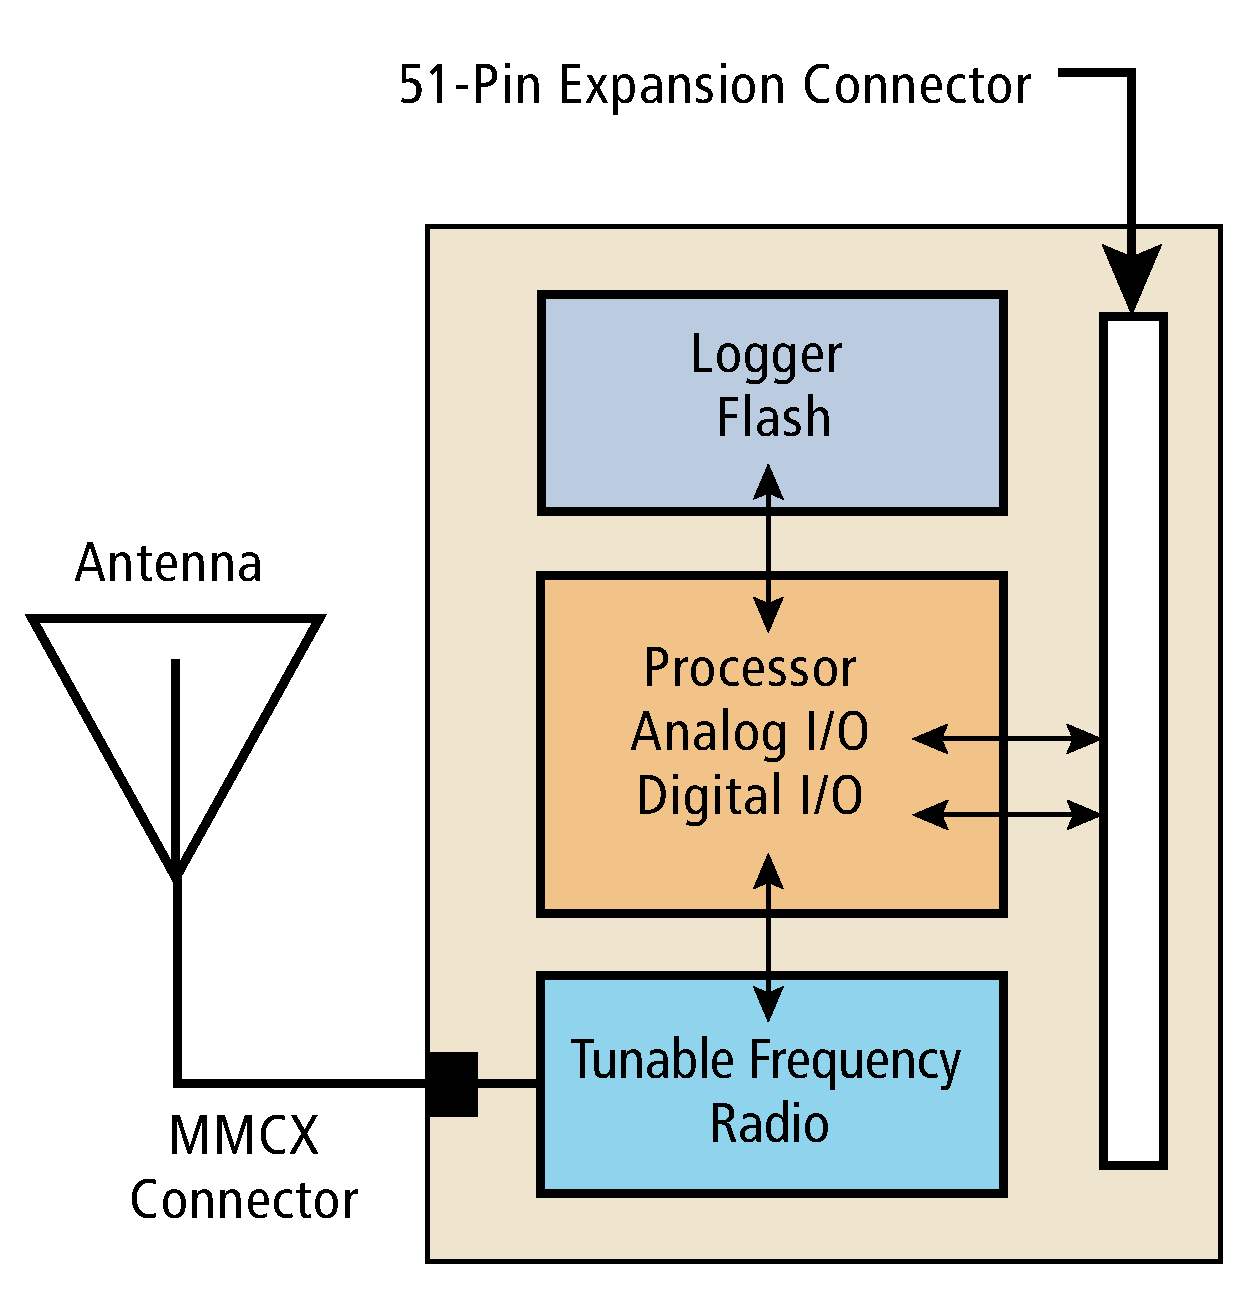
\includegraphics[width=2.8in]{figures/mpr400.eps}}}
\caption{Mica2 sensor and the block diagram.}
\label{fig:mica2}
\end{figure}

The sensor nodes are mainly equipped with processors, sensing devices and communication transceivers. Because they have limited power supply from their batteries, sensor nodes~\cite{mica2-power, micaz-power,telos,telosb} are equipped with a single low power consumption processor. 
For example, a Mica2~\cite{mica2-power} mote shown in Figure~\ref{fig:mica2}, is equipped with an 8MHz ATmega128L processor to process the sensed data.

Due to technological advancement, sensors equipped with multiple chips~\cite{imote2} have been proposed recently. Shown in Figure~\ref{fig:imote2}, Imote2~\cite{imote2} developed by Intel has a digital signal processor (DSP) chip on the mote, in addition to the CPU core, to support image and video operations. The multi-chip sensor is now able to pre-process the multimedia content sensed by the equipped camera and microphone, so that the package that needs to be sent back to the sink contains only a summary of the sensed results.

\begin{figure}[h]
\centering
\mbox{\subfigure[Imote2 sensor]{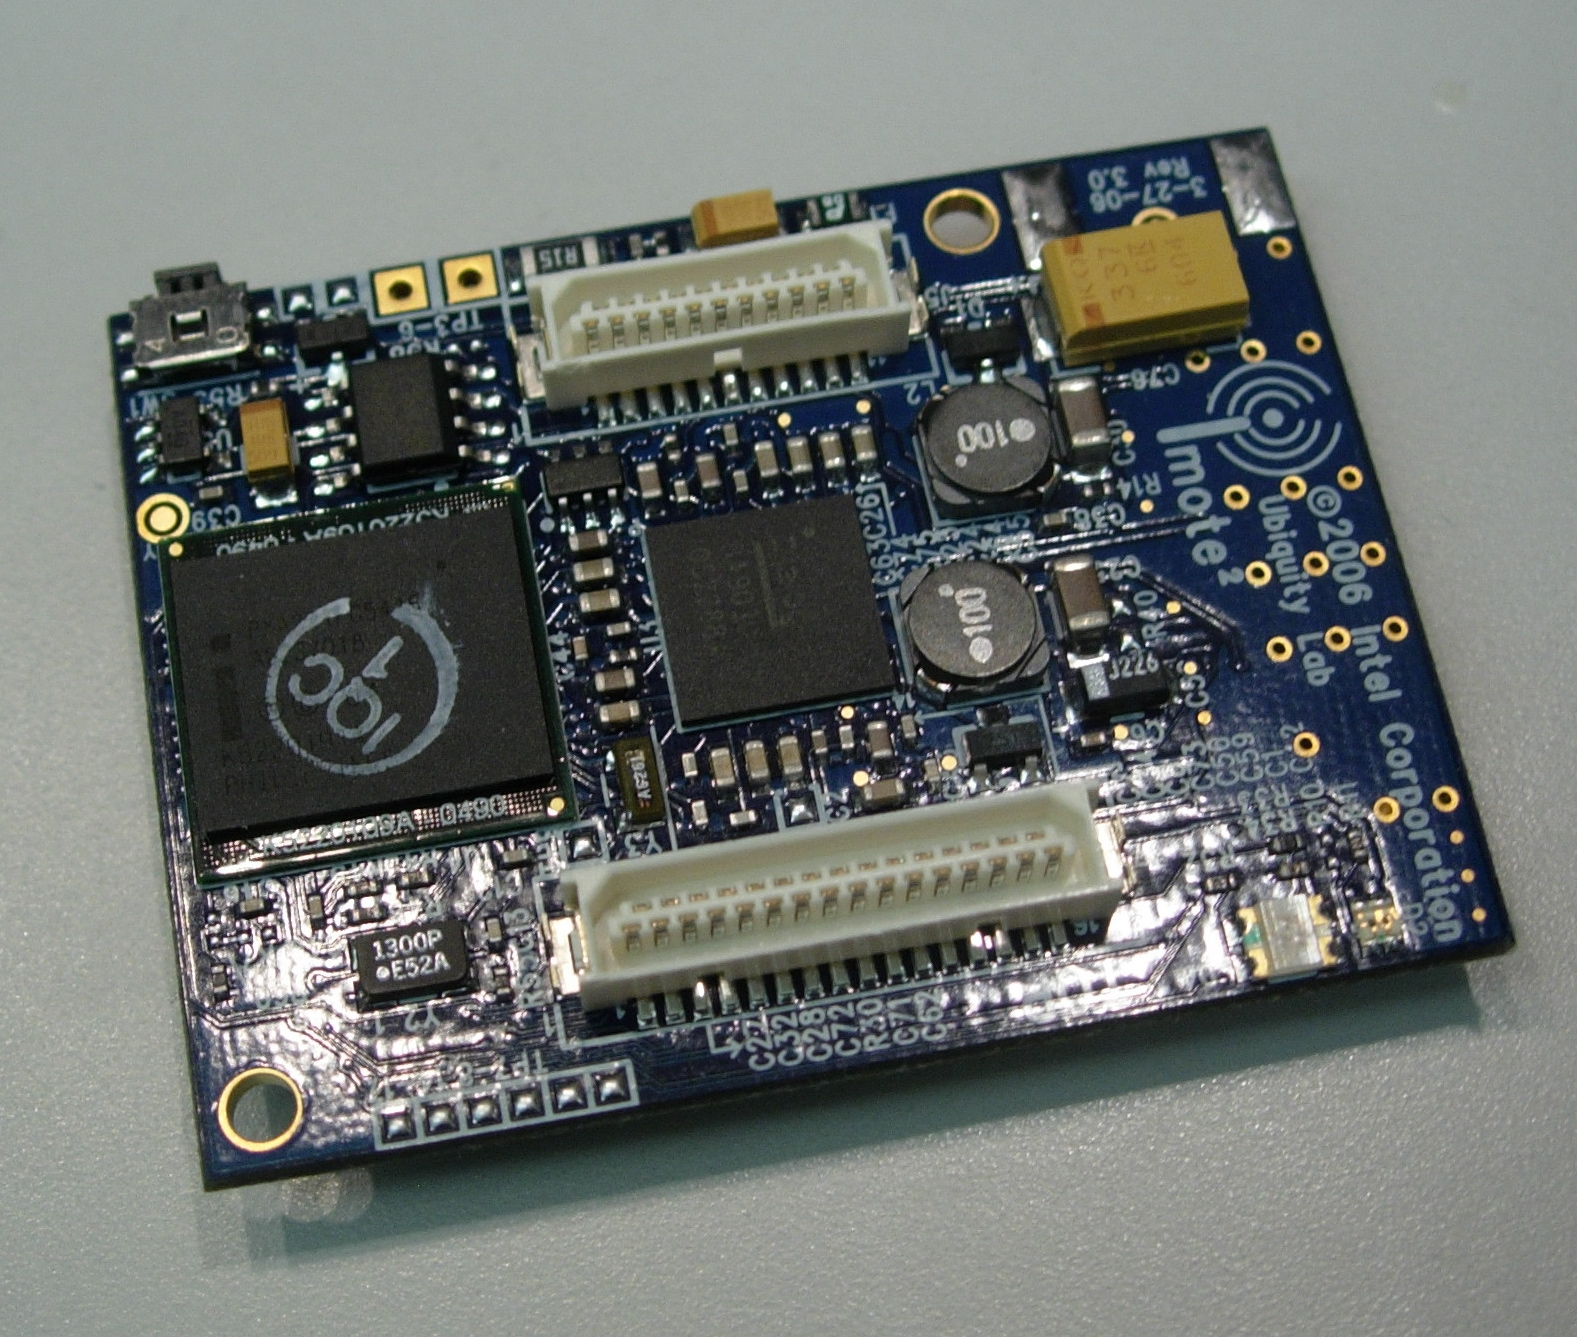
\includegraphics[width=1.8in]{figures/imote2.eps}}
	\hspace{20mm}
      \subfigure[Imote2 block diagram]{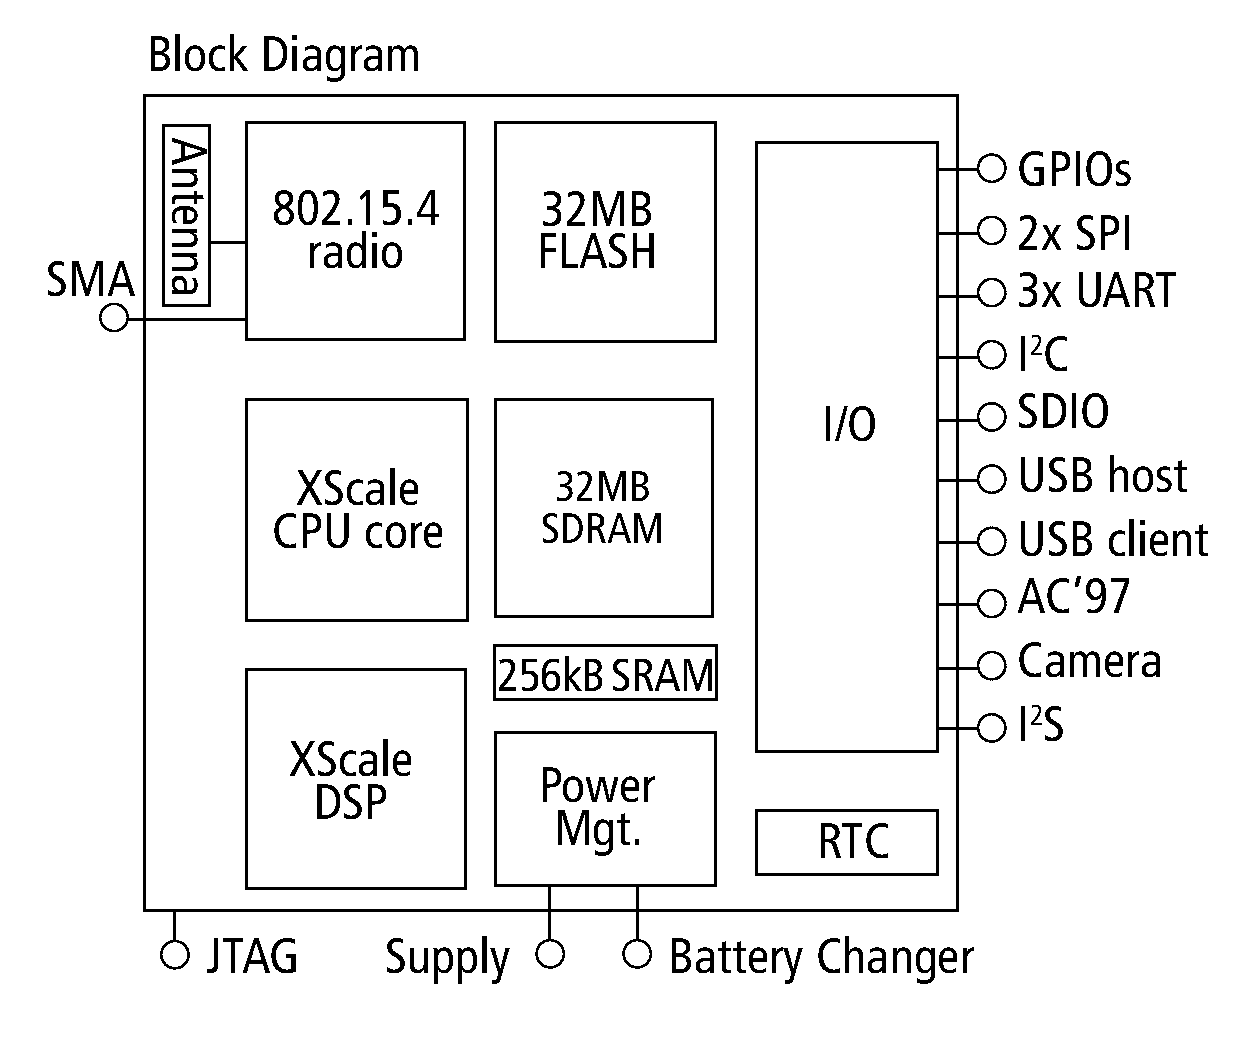
\includegraphics[width=2.8in]{figures/imotedia.eps}}}
\caption{Imote2 sensor and the block diagram.}
\label{fig:imote2}
\end{figure}

The availability of multi-chip sensors poses various design challenges. The high manufacturing cost of these sensor nodes makes it economically less appealing to let the whole network run just one application. Recently, researchers have envisioned the wide adoption of multi-application wireless sensor networks (MA-WSNs), which can support application concurrency in one network infrastructure~\cite{melete,ma-wsns}. Furthermore, MA-WSNs are able to interleave different applications on one sensor node.

Compared to single-application wireless sensor networks (SA-WSNs), MA-WSNs have many advantages in efficiency and flexibility.
For example, MA-WSN can be deployed in a national park to monitor both wildfires and animal movement. A greater proportion of sensors can be set to monitor animal movement during seasonal migration, and more sensors could be set to monitor wildfires during the summer, when wildfires are more likely. By using the same network infrastructure for both applications, MA-WSNs achieves two goals. First, they lessen the investment needed to deploy multiple sensor networks in the same area; and second, they can adapt to the changing environment and adjust coverage according to need.

\textbf{Software upgrade.}
In both SA-WSNs and MA-WSNs, the applications running on the sensors may need to be upgraded after the deployment.
Bug fixes and feature enhancements are the common reasons for software upgrades.
Updates are particularly frequent when applications are still under development because testing and debugging may take several rounds until the code is stable.
For example, the WSN may be deployed in an unfamiliar area so that preliminary data may help scientists better calibrate their sensing applications. I formulate {\em software upgrade problem} as the problem of updating code or data of a running application in a WSN. As shown in Figure~\ref{fig:upgrade}, software upgrading involves binary code generation on the sink node, patch deployment and image replacement on the sensor nodes.
\begin{figure}[htbp]
	\centering
		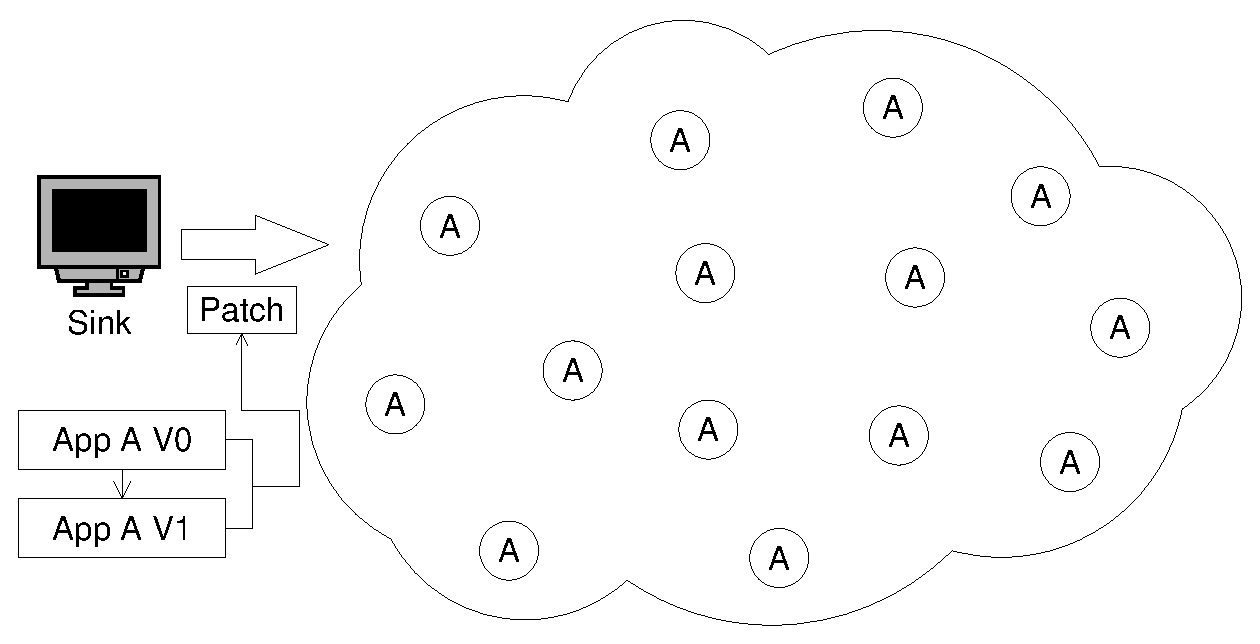
\includegraphics[scale=0.45]{figures/upgrade.eps}
	\caption{Software upgrade in a WSN.}
	\label{fig:upgrade}
\end{figure}
Because the sensors are usually left unattended after deployment, the patch deployment can only be done via wireless communication.
 This is an expensive operation in WSNs. For large WSNs, where the code source cannot reach destinations via broadcasting, the package has to be transmitted hop-by-hop in the network, which consumes a significant amount of energy. A recent study~\cite{related:barr-energy} has shown that the energy used per bit sent over one hop in a WSN is about the same the energy used when executing 1000 instructions. As the sensor nodes are running with limited power supplies, it is essential to conserve the energy in a WSN during software updates, especially when such updates are frequent.
 
One possible solution to this problem is to reduce the number of bytes that need to be transmitted during software upgrades. Because the update patch is actually the binary level difference between the old and new code image, minimizing the binary level difference while generating the new binary will reduce the patch size, thus reducing the energy consumed during the transmission of the patch in the WSN. Patches can also be formatted to reduce their sizes.
A good patch distribution protocol can also reduce the energy consumed in the software upgrade procedure.


\textbf{Software switch.}
For SA-WSNs, software upgrade is the major reason to update the binary image on the sensors, but for WA-WSNs, there is another code update circumstance that can happen.
In order to support application concurrency, multiple code images can be preloaded to the sensor nodes before deployment, and the sensors are able to switch between them upon request from the sink node. However, because of the memory size limitation, not all of the code images can be stored on the sensors. This will require the sensors to fetch the binary of the wanted yet unavailable application from somewhere else. The source can be the sink node, or the neighboring sensors that own this code image. Shown in Figure~\ref{fig:switch}, while doing software switch, only a subset of the sensors in the network need to download the application.
This is different from the case of software upgrades, where all the sensors need to download the new image. Also, both the sink node and the other local sensors may act as code sources, while in a software upgrade, only the sink node can be the source.
\begin{figure}[htbp]
	\centering
		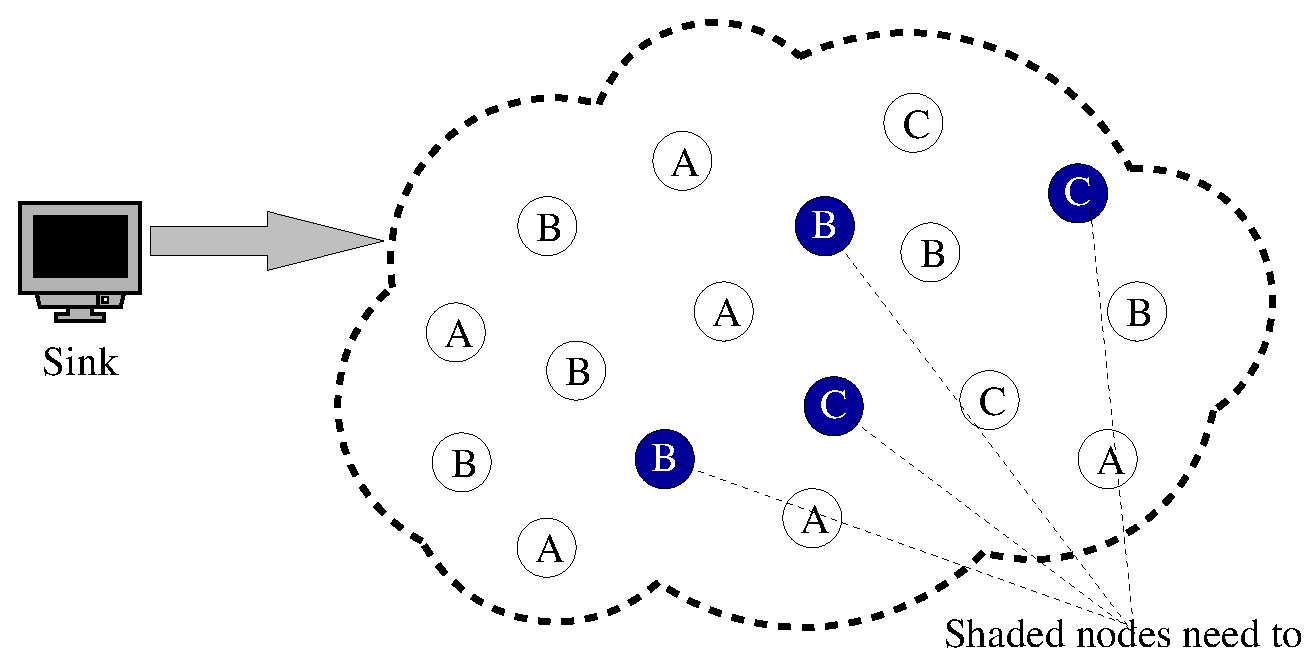
\includegraphics[scale=0.45]{figures/switch.eps}
	\caption{Software switch in a WSN.}
	\label{fig:switch}
\end{figure}

As in the software upgrade problem, in order to reduce the energy consumption during the software switch, an energy-efficient patch routing design and a good patch format design are both desired. 
As different sensor applications may share the same components, there are usually identical parts between the binaries of those applications. For example, in the sensor operating system TinyOS~\cite{tinyos}, there is a component called ``Leds'' that manages the led lights installed on the sensors, and this component is commonly used in many sensor applications such as ``Blink'' and ``CntToLeds''. 
One possible solution is to generate the same binary for the shared part, and use differential patching to transmit only the binary difference between the two applications rather than the entire new binary.

As discussed above, both software upgrades and software switches can happen frequently in WSNs. The patch transmission heavily relies on wireless communication, so it is a costly execution in WSNs.
One of the great benefits that WSNs provide is spontaneity. Once the WSN is set up, it can sense and report
the environmental information automatically.
However, the high power consumption in the software update procedure will affect the lifetime of the WSN.
As the sensors are usually hard to access after deployment, it may be difficult or even impossible to replace their batteries. New sensors may be purchased to replace the old ones, but this is neither economical nor environmentally friendly.

\section{Overview of this research}

Regardless of whether the software update is caused by a software upgrade or a software switch, there are three steps in the software update procedure.
First, the compiler generates the binary image(s).
Second, the patch generator produces the patch.
Third, the patch is disseminated to the WSN.
After each sensor receives the complete patch, it will rebuild the target binary, load it to program memory and start running it.

In order to solve the software update problem in WSNs under all the resource constraints, this dissertation presents a software update management framework, as shown in Figure~\ref{fig:overview}. 
The sink node represents a computer server that is not resource-constrained. The sensor network consists of a large number of sensor nodes with resource limitations in energy, memory size, network bandwidth, time, and CPU.

\begin{figure}[htbp]
	\centering
		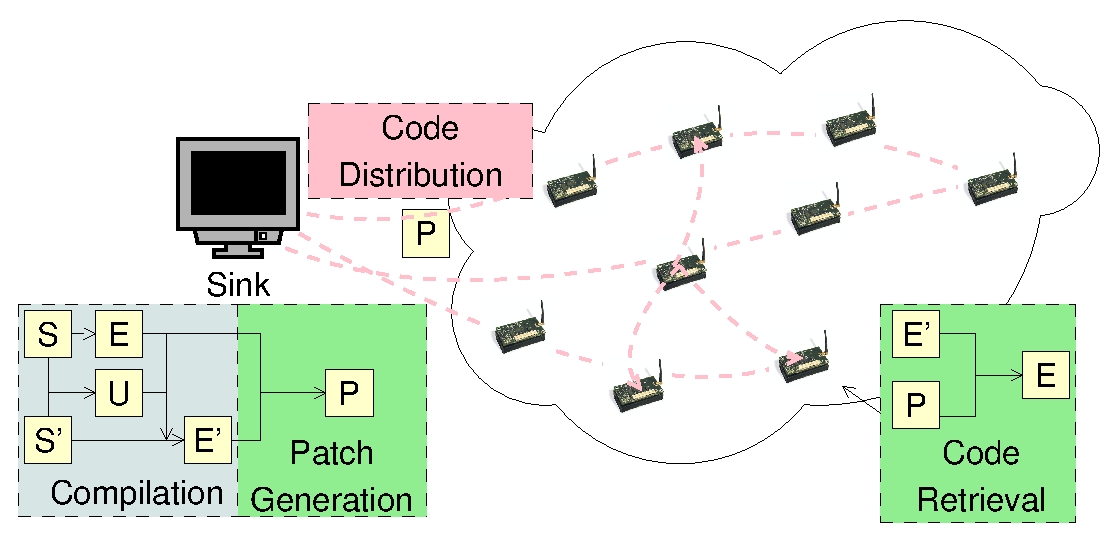
\includegraphics[scale=0.45]{figures/model.eps}
	\caption{Software update framework overview.}
	\label{fig:overview}
\end{figure}


The compiler first compiles the source code into an executable binary {\it E'}. 
Instead of sending the new binary image, a small patch {\it P'} that contains only the difference between {\it E'} and the original binary {\it E} is distributed over the network.  After code distribution is complete, the target sensor regenerates the new binary code {\it E'} by combining the received patch {\it P} and the preloaded binary base {\it E}. 

This framework includes three major components.

\textbf{Update-conscious compiler.} 
Because the patch transmitted over the network is the binary level difference between the old binary and the new  binary, increasing the binary level similarity between the two versions can reduce the number of bytes that need to be transmitted. Therefore, it will save both energy consumption and transmission time in software update. 


In the new version of the source code, the source level statements can be divided into two categories, changed statements and unchanged statements.  The modified source statements will produce binary level differences, and these binary changes are difficult to avoid, yet the source level statements that are not changed may also create binary differences.
This is because in the code generation phase, the compiler may produce different binaries that have the same semantic meanings.

In this dissertation, I will propose update-conscious compiler (UCC) techniques that read the old source and binary to get the compilation choices of the old version, and use them as hints while generating the new binary. 
Shown in Figure~\ref{fig:overview}, the UCC takes {\it E} (the old binary), {\it U} (the intermediate level differences between the old version and the new version), and {\it S} (the new source code) as inputs, to generate the new binary {\it E'}. A similar compilation option is chosen while generating the new binary; thus, this technique can improve the code similarity between the old and new binaries.

This dissertation focuses on the UCC register allocation and data allocation schemes for general purpose and DSP applications.
It proposes ILP-based UCC register allocation (UCC-RA) and heuristic-based UCC data allocation (UCC-DA) for general purpose compilation.
The incremental coalescing single/general offset assignment algorithms are designed for the DSP compilation as the UCC data allocation and UCC address register allocation schemes.

The goal of a UCC is to minimize the binary level differences, so it may not generate code that runs as efficiently as code generated by the conventional compilers.
In fact, a UCC trades the run-time code performance for binary similarity; it saves energy during software updates but wastes energy during the run-time.
If we consider the total energy consumed during both the software update and the execution before the next update, a UCC may not save the energy for the whole procedure and prolong the WSN's lifetime.
In order to solve this problem, I studied the trade-off between the binary code differences and run-time performance. An adjustable UCC scheme is presented in order to achieve the a good trade-off and optimize for total energy use.
	
\textbf{Patch generator.}
After the new binary {\it E'} is generated, it is then compared with the old binary {\it E} to generate the update patch. The binary level differences are described in a highly condensed script {\it P}. 
From the preliminary experimental results, I found that multiple binary level differences can result from the same cause, e.g., instruction insertion or removal can cause destination address shift for the branch instructions.
Including the common cause instead of the individual changes should be able to reduce the patch size.
However, if the update script design is too complicated, it will require more effort on the sensor side to decode and regenerate the target new binary.
This dissertation presents several sets of the script primitives, and discusses the trade-off between the patch transmission effort and the sensor side decoding effort.


\textbf{Code distribution protocol.}
The code distribution protocol disseminates the patch packets to the destination sensors that need the software update. The code source can be either the sink node or the other sensors that own the requested binary image.
This dissertation presents 
a code distribution scheme that works for both software upgrades and software switches.

The presented network protocol also runs under the WSN constraints.
The wireless links in WSNs are not stable. Both the communications and nodes are unreliable because of the environment where the WSN is deployed and the limited energy resources of the sensors. Therefore, the network protocol has to be robust enough to tolerate link failure and node failure.
Because of the high bandwidth and memory usage, the sensors may not be able to perform the sensing applications during the software update procedure. In order to reduce the down time of the sensors, the software update procedure is desired to be as fast as possible. 
Thus, the code distribution protocol design should disseminate the patch scripts through the WSN as quickly and with as little traffic as possible.

%\section{Challenges}
%
%In this research, I focus on the WSNs, that are built with low-power sensors such as the Mica2 sensors~\cite{mica2-power}. They consist of a 8 MHz ATmega128L processor, 128KB of program memory, 512KB EEPROM, 4KB of data memory, and a multi-channel radio capable of transmitting at 38.4 Kbps with an outdoor transmission range of approximately 500 feet. The device measures 2.25 inch $\times$ 1.25 inch $\times$ 0.25 inch and is typically powered by two AA batteries.
%
%The major constraints of designing an energy-efficient software update management framework for such kind of sensor networks are addressed as below.
%
%\textbf{Energy constraints.}
%The environment usually makes it hard to physically access the sensors after deployment, so it is difficult to replace the batteries for the sensors. Recharging the batteries using natural energy sources is not trivial, because the network might be set up in the area, such as the deep ocean, where it is hard to get access of sun light or other natural energy sources. 
%
%Take the Mica2 sensor as an example. The energy contained in each AA battery is 15,390 Joule~\cite{battery-energy}. The experiment results in the recent study~\cite{power-tossim} showed that the energy consumption of the selected applications running on the sensors varies from 153.7 to 3,689 J/day, which makes the life time of the sensors to be 8 days to 200 days. Thus, developing an energy-efficient software update method is very important for energy limited WSNs.
%
%
%\textbf{Memory constraints.}
%The active program is stored in the program memory of a sensor node, while the other inactive programs are stored in the external flash memory. Sensor nodes will load the code image from the external flash to the program memory when they need to switch the running application from one to another.
%
%However, due to the limited size of the external flash memory, the sensor node may not be able to store the complete code images of all the applications that it needs to run. This requires the sensor node to download the unavailable code image from the sink node or the other neighboring nodes during software switch. How to design an energy-efficient code fetching scheme is a problem that we need to solve.
%
%Although the sensors can fetch the wanted code image upon request, the limited sensor memory still needs to be divided wisely to store multiple code images. When the memory is not big enough to hold all the code images, an eviction scheme will be needed.
%
%
%\textbf{Computation constraints.}
%A sensor node is typically equipped with MHz (instead of GHz) micro-controller(s), which limits the complexity of  applications running on it. Therefore, the software update application that runs on the sensors has to be lightweight.



\section{Assumptions}
The following assumptions are made to simplify the implementation of the software update framework in WSNs.

\textbf{Multiple software update procedures on one sensor do not interleave with each other.}
Although it is possible that multiple applications can co-exist on one sensor node, there is a small chance that the software update to these applications happens at the same time.
Also, because the sensors can only run one application at a time, it is not necessary to update them at the same time.
Update sequence can be determined by the order of release time or the execution frequencies.

\textbf{The binary is transmitted during software update.}
A typical compiler like GCC can take over 100K memory space, so it is not practical to install compilers on the sensors.
Therefore, we cannot send the source code to the sensors and let them compile the new binary.
Some designs let the sensors run virtual machine instructions or high level instructions instead of the binary instructions in order to reduce the code size~\cite{mate,related:dynamic1, related:dynamic2}. However, these methods introduce some run-time overhead, which may not be acceptable for a tightly resource-constrained embedded system, so optimizing the software update procedure for the virtual machine design is not discussed in this research. However, it is a future research opportunity.

\textbf{The mapping between the source code and the binary can be built.} Compiler optimizer may re-order the instructions in order to achieve better run-time performance. Therefore, the update-conscious compilation techniques should execute as a separated pass after the other compiler optimizations. 
We assume that the compiler can create the mappings between the optimized binary statements and the source statements to categorize the binary level differences into the functional changes and nonfunctional changes.
The update-conscious compiler will then decrease the amount of the nonfunctional binary changes.
Mappings between the unoptimized and optimized statements can be created by using the technology proposed by~\cite{mapping}.


\textbf{The number of executions of one application can be estimated.}
As the software engineers who design the application should be able to estimate how often one execution can be trigged, and the lifetime of one application can be estimated by the historical release logs, the number of executions that one application will do before retiring can be estimated. This number acts as a constant for each application in the energy consumption formula, and determines the compilation strategy that will be used to generate the binary in the adjustable UCC algorithms.

\section{Organization of this dissertation}
The remainder of this dissertation is organized as follows. 
Chapter 2 presents background information on the general WSN software update and the three components of 
the proposed framework, including traditional register allocation,
data allocation design, WSN software update script primitive design and WSN code dissemination protocol design.
Also, the relationship of this dissertation and prior work is discussed. 
Chapter 3 discusses the proposed UCC design, including the UCC register allocation and data allocation for
general purpose applications and the UCC data allocation and address register allocation for DSP applications.
Chapter 4 presents the script primitives that are used to summarize the binary level differences
in the update patch.
In Chapter 5, the patch distribution protocol is presented. 
Chapter 6 presents the experimental results and discusses the trade-offs.
Chapter 7 addresses the directions for future
research and the conclusion.

\chapter{Background and related work}\label{chap:related}

In this section, I will first give some brief introduction to the related research about software update in WSNs, and then I will describe some background research that is related to the major components of my proposed framework.

%\section{Control Logic}

\section{Software update in WSNs}

The existing WSN software update designs can be categorized according to {\em what} is to be transmitted over the network. 

The simplest solution is to transmit the complete new binary image to replace the old one on the sensors, e.g., Deluge (the default code distribution scheme in TinyOS~\cite{tinyos}).
The proposed schemes in this category mainly focus on how to package the new binary image and route the packets to the sensors under WSN constraints.
However, since the new binary and old binary share some common code segments, transmitting the complete image is not necessary and is a waste of energy.

Another approach is the {\em diff}-based design, which compares the code of successive versions and generates an edit script that summarizes the differences.
Only the script is transmitted to the remote sensors where the new code is re-generated by combining the old image and the edit script.  Since
less data is transmitted over the network, and the edit script is usually simple and can be easily interpreted by the sensors, the {\em diff}-based approach significantly improves energy-efficiency and has
become more popular in WSNs~\cite{related:script,stream,related:jeong-script,related:dynamic1,related:dynamic2,related:flexcup}.
The major focus of this category is how to compare the two binary versions and generate a small edit script.
However, because the code differences are derived from binaries generated using the {\em conventional compiler's code generation methods}, with possibly some optimizations, a simple change in the source code may result in many changes in the final binary. This has limited the {\em diff-}based approaches to only small updates such as fixing a ``bug''~\cite{related:script}.


The third approach transmits the binary code at different levels.  Some recent work introduced a small virtual machine~\cite{mate} or a dynamic linker~\cite{related:dynamic2,related:dynamic1} on the remote sensors. Instead of binary instructions, the code is represented at a higher level, e.g., virtual machine primitives,
which can minimize the code difference in many cases. The tradeoff is that these approaches introduce high runtime overhead and may consume more energy in the long run.


\section{Compiler}

Compiler is a program that can read a program in one language -- the \textit{source} language -- and translate it into an equivalent program in another language -- the \textit{target} language.~\cite{compiler}
The work flow of a compiler is shown as Figure~\ref{fig:compiler}.

\begin{figure}[htbp]
	\centering
		\includegraphics[scale=0.45]{figures/compiler.eps}
	\label{fig:compiler}
	\caption{Compiler work flow}
\end{figure}

The \textit{front-end} analyzes the source code to build an internal representation of the program, called the \textit{intermediate representation} or \textit{IR}. The \textit{IR} then is transformed into functionally equivalent but faster (or smaller) forms in the \textit{optimizer}. At the last stage, \textit{code generation}, the \textit{optimized IR code} is transformed into the target machine binary.

My study~\cite{ucc} has shown a small local source code change might cause a big difference in the binary. This is because if the source code level difference is minor and local, when translating such source code into IR code, the difference will also be localized, assuming a one-one mapping can be created between the source code and IR code. However, transforming the IR code to the target binary code may propagate such local differences into global differences, by applying data allocation, code placement, register allocation, etc. Thus, my update-conscious compilation design will focus on the code generation pass. The goal is to let the compiler preserve the semantic meaning of the source program while generating a similar code image with a given code image. Two key problems in code generation, register allocation and data allocation are studied in this research.

\subsection{Register allocation}

Registers are the fastest computational unit on the target machine, however, usually there are less registers than the values that need to be held. The goal of register allocation is to determine what values should be held by what registers. Because the values that are not held in registers reside in memory, and memory access takes longer time compared to register access, the efficiency of register allocation algorithm affects the execution efficiency of the program. 
Finding an optimal assignment of registers to variables is mathematically NP-complete. However, in the past twenty years, the register allocation problem has been extensively studied with great success in many aspects. 

\textbf{Traditional register allocation schemes} Graph coloring algorithms construct the variable interference graph and solve the global register allocation as a graph coloring problem~\cite{related:graph-color,related:graph-color-improvements,related:graph-color-iterated,related:graph-color-priority}. To achieve fast compilation, linear-scan algorithms assign variables to available registers through a simple scan of the program, instead of constructing the interference graph~\cite{related:linear-scan,related:linear-scan-fast}. It was reported that linear-scan allocators generate similar performance level code as those from graph coloring-based allocators, with a shorter compilation time required. Recently, the optimal or near optimal register allocation was formulated and solved through integer linear programming~\cite{related:ilp,related:ilp-cisc,related:ilp-fast} or multi-commodity network flows~\cite{related:ilp-progressive}.

However, all these register allocation algorithms listed above, target at generating code with better performance, in terms of less register spills. In the WSN software update management concept, we want to design an update-conscious compilation technique in order to reduce the size of update between different versions of one program or two programs that share common components. So these traditional register allocation schemes do not fit in our requirement.

\textbf{Update oriented register allocation}
Bivens and Soffa proposed the Incremental Register Allocation (IRA) scheme~\cite{related:ira} based on traditional graph coloring algorithm. While the software is update incrementally based on a previous version, the scheme only reallocates registers for the changed code, but preserves the assignment for unchanged code. 

Though it is designed for incremental compilation, its goal is to save compilation time, when minor software update occurs. It may generate similar register allocation results as the previous version unintentionally, yet it always follows the original register allocation for the unchanged code, which may lose the code performance when the source code update is relatively large. Thus, even though such code similarity may cause energy saving in code distribution stage, more energy will be consumed in the future execution.

So besides considering the code similarity, the update-conscious register allocation scheme should also be adaptive to both small and large source code updates. The design goal is to achieve optimal overall energy consumption, which includes both code dissemination and future code execution. 	

\textbf{Code compression oriented register allocation}
Ros and Sutton proposed a post-compilation register reassignment technique~\cite{related:register-reassignment}. It creates the mappings of the registers that are used in isomorphic instructions, and tries to replace one register with its mapping register. The design goal is to increase the code similarity between different components within one program, in order to improve Hamming distance based code compression~\cite{hamming-compress}. 
The idea can be borrowed to design update-conscious register allocation techniques. However, when the paired register is not available for the register replacement, the register replacement will be aborted. 

\textbf{Summary}
While doing software update in WSNs, we need the compiler to consider register assignment similarity, as well as the code performance. The update size and execution frequency of the updated software should be considered to balance the performance loss and the code similarity improve, in order to achieve the overall energy saving.

\subsection{Data allocation}
Data allocation assigns memory location for each variable in the program. Research has shown that the data allocation may also affect the code performance and code size~\cite{related:liao, related:bartley}.

\textbf{Addressing code generation in DSPs}
Modern multi-chip wireless sensors have integrated DSP processors to support multimedia applications that process audio, video and communication signals. DSP processors strive to achieve low cost, low power, and low latency digital signal processing by integrating specially optimized architectural components. For example, a dedicated Address Generation Unit (AGU) can perform parallel address computation in {\em register-indirect} addressing mode. With {\em register-indirect} addressing, the memory address is stored in an address register (AR) whose value can be automatically updated within a small range before or after memory accesses. Such update incurs no extra cost. As a comparison, the {\em base-register-plus-offset} addressing requires two instruction words on 16-bit DSP processors e.g. AT\&T DSP16xx~\cite{related:dsp}. By carefully allocating variables in the memory, DSP compilers can generate efficient code with compact size and improved performance.


\begin{figure}[htbp]
	\centering
		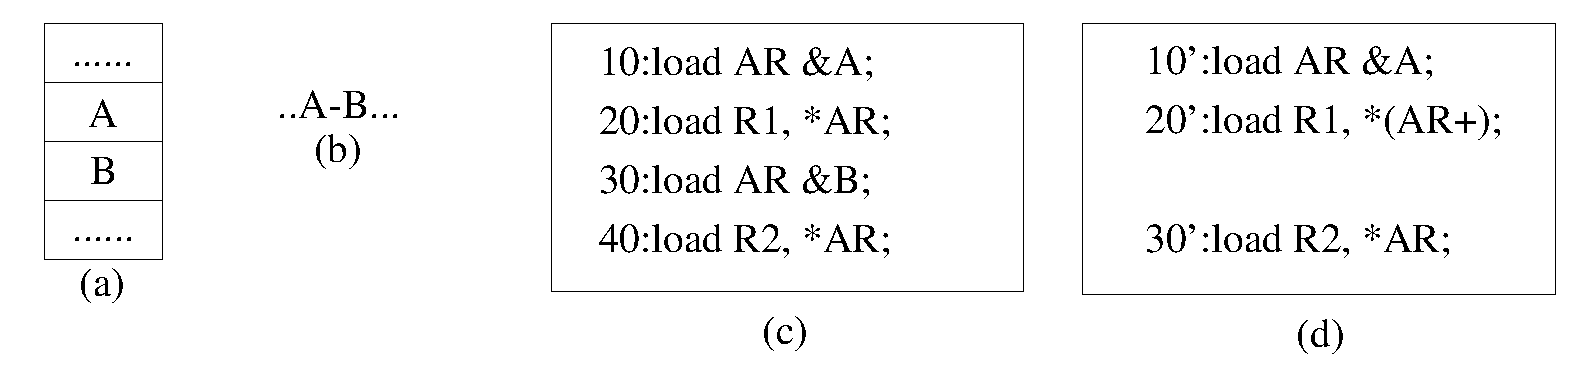
\includegraphics[scale=0.45]{figures/agu.eps}
	\label{fig:agu}
	\caption{Auto-addressing}
\end{figure}

The AGUs on DSP processors assist the address computation in parallel. For the most frequently used auto addressing instructions such as post- and pre- address increment/decrement instructions, no explicit addressing instruction is needed when the address distance of two consecutive memory accesses is smaller than two; otherwise an extra instruction is needed to update the address register (as instruction 30 shown in Figure~\ref{fig:agu}).

\textbf{Offset assignment}
Auto-addressing mode can increase the code performance as well as reducing code size. On the other hand, the memory layout has to be optimal in order to achieve the best code performance and compression. The problem of assigning variables in memory was formulated by Bartley~\cite{related:bartley} and Liao \textit{et al.}~\cite{related:liao} as Simple Offset Assignment (SOA) problem, where there is only one AR, and General Offset Assignment (GOA) problem, where there are multiple ARs. A variety of heuristic algorithms have been proposed later~\cite{related:atri,related:choi,related:leupers-1996,related:leupers-1998,related:ottoni,related:rao,related:sudarsanam,related:zhuang}.

The general solution of SOA is equivalent to finding the maximum weight Hamiltonian path\footnote{A Hamiltonian path in a graph is a path that visits every vertex exactly once.} in the access graph~\cite{related:bartley, related:liao}, where each vertex represents a variable; each edge between two vertices represents there is at least one consecutive access between the two related variables; and the weight of each edge shows the number of times that the two variables are consecutively accessed. GOA problem can be simplified as \textit{N} SOA problems, where \textit{N} is the AR number. 

\textbf{Offset Assignment with variable coalescing}
Since many variables have short live ranges, variables that do not interfere with each other can be allocated in the same memory location, to furthermore reduce data memory size and improve code performance. An efficient offset assignment heuristic using variable coalescing is proposed by Ottoni \textit{et al.}~\cite{related:ottoni} and Zhuang \textit{et al.} ~\cite{related:zhuang}. In each iteration, either an unselected edge is selected to be on the Hamiltonian path, or two vertices are chosen to be coalesced until no more vertices can be coalesced and the Hamiltonian path is built.

The design goal of the current offset assignment schemes is to generate efficient code with compact code size and improved performance. So when the program is slightly updated, the compiler might generate a different coalesced offset assignment compared to the original version. Even though the memory layout difference is very simple, e.g. when there is a simple switch of two variables' memory addresses, all the instructions that access these two variable or the instructions that are adjacent to the memory access instructions of these two variables may need to apply a different addressing mode, which produces many code differences from the original version. 
Thus, while doing software update in WSNs, we need the compiler to consider the memory layout similarity with the previous version of code, as well as the code efficiency and size, in order to reduce the patch size during software update.


\section{Patch generator}

After the code compilation is finished, the sink node generates the patch code based on the binary code before sending out the patches. There are several ways to prepare the patches.

\textbf{Compression}
Compression algorithms, such as bzip2, compress, LZO, PPMd and zlib, can be used on the generated binary code to reduce the patch size. Simply using these existing compression algorithms on the binary code generated by the compiler can reduce the patch size by 20\%~70\%. Even though it can help reduce the transmission power consumption, these high compression ratio algorithms also requires a lot of computation to retrieve the original code. Experiment results~\cite{related:barr-energy} show that bzip2 requires to run 31 instructions to restore 1 bit, which makes the code decompression very expensive.

\textbf{Differential patching}
When an update is an incremental improvement on a deployed function, such as bug fix or parameter change, the new image is often very similar as the old version. So instead of transmitting the complete image of the updated/new application, a differential patch between two images can be transmitted as the update. 
%An update script can be used to describe the differences~\cite{related:script, related:jeong-script, ucc}.
%After sensors receive the patch packets, they copy part of the code from the old image and part of the code from the patch, to form the updated binary.
However, this method only works well for small updates. When the update is relatively big, the patch size may be big.
%My study has shown that a simple source code level update can trigger big binary level differences, such as data allocation switching, register assignment switching and target address switching. For example, Reijers \textit{et al.} proposed a new script command called ``patch list'', which shifts the target address in the old image with an offset while copying the instruction to the new image.

Differential patching scheme can be used in our WSN software update framework design, because the update-conscious compilation technique could reduce the image differences. As discussed before, a small register assignment or data assignment change could cause a big difference in the generated target code, which may affect several instructions. The current differential patching schemes only show the instruction level differences in the script, which may need to incorporate multiple instruction changes in the update script. However, if the context-aware information, such as register assignment change or data assignment change is provided in the script, the sensors may be able to update the binary code by itself, which can significantly reduce the update patch size.

\textbf{High level instruction}
Patching code at higher semantic levels tends to generate smaller update script. Levis \textit{et al.} showed that the code size is very short when they are represented using virtual machine instructions~\cite{mate}. Marr\'on \textit{et al.} proposed a scheme to produce separate object files for TinyOS~\cite{tinyos} components and linked by sensors~\cite{related:flexcup}. Dunkels \textit{et al.} further proposed a dynamical linker for this systems~\cite{related:dynamic1}. Koshy \textit{et al.} proposed to relocated modules and generate the binary using a remote linker~\cite{related:dynamic2}.
A drawback of releasing code not in the binary format but the higher level language is that it requires extra runtime overhead, which might be not acceptable for tightly resource-constrainted embedded system.

\section{Distribution protocol}

After the patch generation stage, the patches are ready to be distributed over the network. Many code distribution protocols have~\cite{spin,trickle,melete,deluge,mnp} been proposed.

\textbf{SA-WSN code distribution protocol}
In SA-WSNs, all the sensors run the same application, so the distribution protocol design in SA-WSNs focuses on the efficient flooding scheme, which sends the patch packets to all the sensors in the network. The original efficient data flooding scheme in WSN, called SPIN~\cite{spin} uses a three-way handshaking protocol, shown in Figure~\ref{fig:spin}. Each sensor broadcasts the software information (ADV messages) as advertisements. The sensors that need to update its software send a request (REQ) message to the code owners. And then the code owners respond with the DATA messages.

\begin{figure}[htbp]
	\centering
		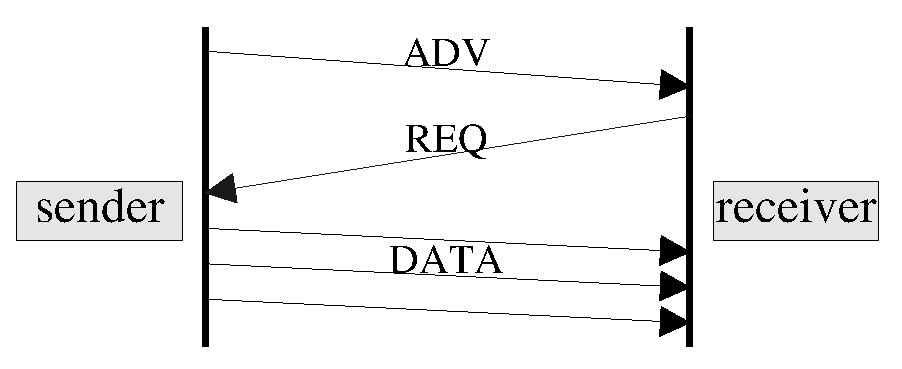
\includegraphics[scale=0.4]{figures/basic-protocol.eps}
	\label{fig:spin}
	\caption{Basic code distribution protocol (SPIN)}
\end{figure}

Trickle~\cite{trickle} improves SPIN by adding periodical advertisement feature, which reduces the energy used in the advertise phase. Deluge~\cite{deluge} extends Trickle to support efficient flooding of large data especially code images, by dividing big code image into fixed sized segments, and the transmission of different segments can happen simultaneously in the network for rapid code prorogation purpose. 


\textbf{MA-WSN code distribution protocol}
Because MA-WSNs support concurrent multiple application execution, only part of the sensors may be interested in the new code image. So a pull based multicast scheme should be used. Melete~\cite{melete} protocol only sends the code image to the sensors that request it instead of broadcasting it to all the sensors. Besides that, multihop code dissemination is also supported. The weakness of this scheme is that it relies on the request message to discover the routing to the source node, which may cause request message flooding in the network.



 \chapter{Goals and approaches}\label{chap:goals}
The overall goal of this research is to design an efficient software update management system for both SA-WSN and MA-WSN. The efficiency here means that the system has to satisfy the resource constraints of WSNs, with a lower power consumption. To achieve the main goal, each major component in the software update management framework needs to be modified with novel techniques and algorithms to address the challenges described above. The abstracted framework is shown in Figure~\ref{fig:framework}.

\begin{figure}[htbp]
	\centering
		\includegraphics[scale=0.45]{figures/framework.eps}
	\caption{The abstracted framework.}
	\label{fig:framework}
\end{figure}

The components that require modifications are:
\textbf{Compiler}
Instead of using a traditional compiler, an update-conscious compilation (UCC) technique is deserved in the WSN software update. Besides the code performance, the code similarity with another code image needs to be considered as well. 
The proposed UCC technique involves UCC register allocation (UCC-RA) and UCC data allocation (UCC-DA).

\textbf{Patch generator}
A patch generator is then used to summarizes the binary level code differences in a highly condensed style. Instead of explicitly listing the instruction level differences in the patch, the code structure changes, such as the register assignment switch and memory layout changes, are addressed directly in the patch script in order to reduce the patch size. 

\textbf{Distribution Protocol}
As mentioned in Chapter~\ref{chap:intro}, I divide the WSN {\it software update} into two circumstances, {\it software upgrade} and {\it software switch}.
While doing {\it software upgrade}, I adopted the existing code distribution protocol Deluge~\cite{deluge} to propagate the software upgrade patches from the sink node to the sensors that need upgrade. 
For \textit{software switch}, I proposed a multi-cast based code distribution protocol to let the sensors download the wanted binary code from the neighboring nodes that have the code image in memory. A dynamically updated routing table is used to guide the routing of the code requests to reach the source nodes.


The design goals of the software update framework are:
\begin{itemize}
\item reduce the overall energy consumption in software update.
\item reduced overall time consumption in software update.
\item the code dissemination protocol and the code retrieval algorithm run on the sensors have to obey the sensor network constrains, discussed in chapter~\ref{chap:intro}.
\end{itemize}

The design goals of this proposal will be accomplished by completing each individual components and integrating them as a complete framework. The design approaches of each framework component are discussed as below.


\chapter{ Update-conscious compilation (UCC) techniques}

The conventional compilation takes the following steps to generate binary code from the source code, as depicted in
Figure~\ref{fover.sink}. First, the compiler converts the source code $S$ into an intermediate representation $ir$. Next, the compiler optimizes the $ir$ for several iterations, and produces the optimized intermediate representation $IR$. Finally, the code generation stage uses $IR$ to generate the binary code $E$ by applying data allocation, code placement, register allocation, etc.
\begin{figure}[htp]
\centering
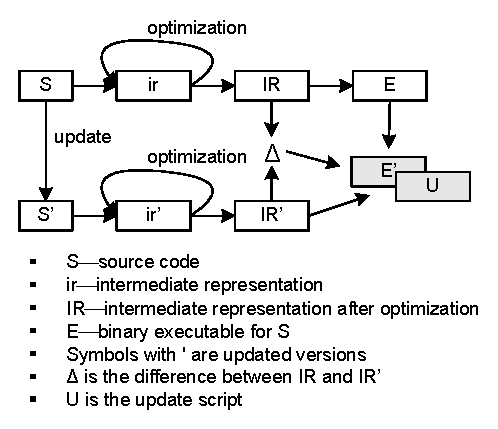
\includegraphics[scale=1]{figures/com_sink.eps}
\caption{The sink-side update-conscious compilation.}
\label{fover.sink}
\end{figure}

The proposed UCC schemes are performed at the code generation stage, i.e. from $IR$ to $E$. This helps to preserve the performance improvements from the optimization passes. 
Three update-conscious schemes are proposed for register allocation and data allocation phase in the code generation stage. For clarity, I assume that the optimization passes are {\it independent} from these two phases, and other optimizations will be investigated in the future work.

When $S$ is updated to $S'$ (Figure~\ref{fover.sink}), $ir$ and $IR$ are also updated to $ir'$ and $IR'$ respectively. Let $\Delta$ represent the differences between the $IR'$ and its previous version $IR$. With $\Delta$, the compiler can analyze and decide how to generate the binary $E'$ such that its difference from $E$, denoted as $U$, is small.

The binary difference $U$ will then be transmitted over the network to the sensors. When the sensors receive the complete $U$, it will construct the target executable $E'$ by combining $U$ with old version executable {E}. This demonstrated in Figure~\ref{fover.sensor}.

\begin{figure}[htp]
\centering
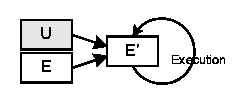
\includegraphics[scale=1]{figures/com_sensor.eps}
\caption{The sensor-side code update and execution.}
\label{fover.sensor}
\end{figure}

\section{UCC for general purpose applications}

In this section, I will discuss about the update-conscious compilation schemes for general purpose applications.
The UCC schemes for general purpose applications include the register allocation scheme, data allocation and
the integrated scheme that combines both register allocation and data allocation.
The goal is to generate the new binary image as similar as the old binary image as possible with the minimal
run-time performance loss. I will discuss the detailed algorithms in this section.


\subsection{UCC data allocation (UCC-DA) for general purpose applications} 

The binary instructions can be updated due to data allocation result changes.
For example, the load/store instructions that access a variable whose memory address is changed,
need to be updated.
Thus, one task of UCC is to improve the data allocation similarity.


\subsubsection{Data allocation problem for general purpose applications}

\begin{figure}[htbp]
\centering
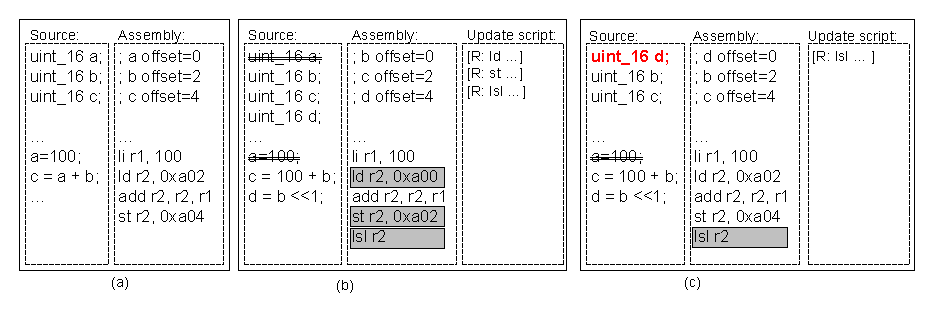
\includegraphics[width=5.5in]{figures/fdata.0.eps}
\caption[An example of incremental data allocation.]{An incremental data allocation example.
(a) Original source and assembly code;
(b) New code and the update script;
(c) Incrementally generated new code with a smaller update script.}
\label{fdata.0}
\end{figure}

The data allocation
strategy can affect the similarity between different versions of
binary, as illustrated in the example in Figure~\ref{fdata.0}.  In the
original code (Figure~\ref{fdata.0}(a)), three variables {\it a, b},
and {\it c} are allocated with offset 0, 2, and 4 respectively, to a
base address. Assume the code is updated by replacing variable {\it a}
with a constant, and introducing a new variable {\it d}. The existing
compiler may generate the data allocation scheme as shown in Figure~\ref{fdata.0}(b), in which all variables are assigned with new
offsets, resulting in three updated instructions. However, an update-conscious algorithm should put the new
variable {\it d} in {\it a}'s old location, as shown in
Figure~\ref{fdata.0}(c), resulting in only one updated instruction. 
On the other hand, if there was no {\it d} in the new code and
if the word taken by {\it a} was not claimed, I would waste the
word in RAM or more if the function is recursively
invoked on the call stack. This will increase the memory usage on remote sensors.


The memory space here refers to the RAM space, 
which is used to store the call stack. A typical wireless sensor has a
4KB RAM (Mica2 or MicaZ), used to store not only the call stack but
also the data segment and the BSS segment. Figure~\ref{ram} shows the sensor memory
model. The size of the data segment and BSS segment can be calculated
by using static analysis, but the stack size changes as the program
executes. In order to make sure that the stack will not overflow,
the worst case stack size counting the memory waste cause by UCC-DA should satisfy the following equation.

\begin{small}
\begin{equation}
\mbox{\it stack region size}\leq \mbox{\it RAM size} - (\mbox{\it data segment size} + \mbox{\it BSS segment size})
\end{equation}

\end{small}

\begin{figure}[h]
\centering
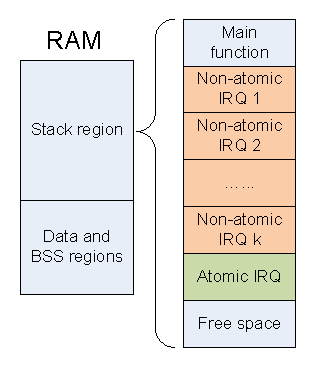
\includegraphics[scale=1]{figures/ram.eps}
\caption{The sensor memory model.}
\label{ram}
\end{figure}

\subsubsection{UCC data allocation for general purpose applications}

To address the problem of how to keep the 
data allocation similarity as well as the worst case call stack
size to be lower than the available RAM size, I propose a {\em
threshold-based data allocation} mechanism~\cite{ucc}.  The intuition is to reuse
the space of the deleted variables as much as possible, and when
there are more new variables than the deleted variables we will create memory 
holes in the functions that have the least affect to the overall memory usage.

\begin{itemize}
	\item If there are more
new variables than the deleted ones, the {\em
threshold-based data allocation} algorithm will first use up the space of the
deleted variables and then allocate more space. 
\item If there are more
deleted variables, some space will be left. 
There are two options to save this space: 
\begin{itemize}
\item relocate some old variables;
\item do not relocate. 
\end{itemize}
The first option
does not waste the space resource on sensor node, but it needs to
change the program code because of the 
variable reallocation. The second
option incurs less code changes but leaves ``holes'' in the call stack 
at runtime. As a hybrid of these two options, the proposed
algorithm keeps the maximal data allocation similarity, under the constraint
that the total wasted RAM space is less than a given threshold --- $SpaceT$. 
This threshold can be calculated by computing the size of each segment 
in RAM using traditional compilation method and subtract that from the RAM 
size.
For ease of illustration, the proposed algorithm
elaborates on the procedures for variables of word type only. The principle can be
applied to other data types such as array and composite structures
similarly.
\end{itemize}

The detailed algorithm is shown in Algorithm~\ref{alg-data}.

\begin{algorithm}
\singlespace
\caption{UCC-DA for general purpose applications.}
\label{alg-data}
\begin{algorithmic}[1]
\singlespace
\REQUIRE Function list $P[]$, the wasted space threshold $SpaceT$.
\ENSURE The data allocation result.
\FORALL{$P_i\in P[]$}
\STATE $TotalWastedSpaceSize \leftarrow 0$;
\STATE $NumOfDelV_i \leftarrow $ the total number of deleted variables in $P_i$;
\STATE $NumOfNewV_i \leftarrow $ the total number of new variables in $P_i$; 
\STATE $NumOfInsts_i \leftarrow $ the projected maximal simultaneous instances of $P_i$;
\IF {$NumOfDelV_i \leq NumOfNewV_i$}
\STATE Reuses all the space from deleted variables;
\STATE Allocate extra space to satisfy the remaining new variables;
\ELSE
\STATE Reuses all the space from deleted variables;
\STATE $ExtraSpaceSize_i \leftarrow NumOfDelV_i$ - $NumOfNewV_i$;
\STATE $TotalWastedSpaceSize$ += $ExtraSpaceSize_i \times NumOfInsts_i$;
\ENDIF
\ENDFOR
\WHILE {$TotalWastedSpaceSize > SpaceT$ }
\STATE $Max\_Factor \leftarrow 0$;
\FOR{$P_i \in P[]$ AND $ExtraSpaceSize_i > 0$}
\STATE $Usage_i(last) \leftarrow$  the usage of the last variable in $P_i$;
\STATE $Factor_i \leftarrow \frac{NumOfInsts_i}{Usage_i(last)}$;
\IF {$Factor_i  > Max\_Factor$}
\STATE $Max\_Factor \leftarrow Factor_i$;
\STATE $To\_Move \leftarrow i$;
\ENDIF
\ENDFOR
\STATE Move the last variable in function $To\_Move$ to fill up a memory ``hole'';
\STATE $TotalWastedSpaceSize$ -= $1\times NumOfInsts_i$;
\ENDWHILE
\end{algorithmic}
\end{algorithm}
\vspace{0.2in}
First, it collects the following profiles for each function $P_i(i\geq
0)$ in the program. 
\vspace{+0.1in}
\begin{small}
\begin{center}
\begin{tabular}{r|l}
$NumOfDelV_i$ & the total number of deleted variables in $P_i$; \\
$NumOfNewV_i$ & the total number of new variables in $P_i$; \\
$NumOfInsts_i$ & the projected maximal simultaneous instances of $P_i$; \\
$Usage_i(a)$ & the usage of variable {\tt a} in $P_i$. 
\end{tabular}
\end{center}
\end{small}

Second, it gradually allocates new variables within each procedure
$P_i$ as shown in Algorithm~\ref{alg-data} line 6$\sim$13. 
Instead of removing the deleted variables directly, it only marks them as deleted variables so that their space can be reused by new variables. If $NumOfNewV_i$ is larger than or equal to $NumOfDelV_i$, it reuses all the space from the deleted variables and allocate extra space to satisfy the remaining new variables. 
If $NumOfNewV_i$ is smaller than $NumOfDelV_i$, i.e., new variables
cannot reuse all space of the deleted ones, then it computes the number of words left to be filled
using the following formular:
\begin{eqnarray}
ExtraSpaceSize_i = NumOfDelV_i - NumOfNewV_i
\end{eqnarray}
and moves to the next step.

In this step, it adjusts the data allocation by incrementally relocating the
{\em last} variable in each function. It keeps moving the last variable into a
``hole'' left by variable deletion, until all the ``holes'' are filled.
That is,
\begin{eqnarray}
\sum_{\forall Pi} ExtraSpaceSize_i \times NumOfInsts_i \leq SpaceT
\label{spacet}
\end{eqnarray}

While deciding which function needs to move the last variable up to fill up the ``hole'', 
functions are ordered by two factors.
One is the number of usages of the last variable $Usage_i(last)$ and another one is the number of instances 
that the function can have on stack $NumOfInsts_i$.

If the last variable in the function is used more often,
such data allocation move will cause more instruction updates, so we want
to move the last variable in the function whose last variable is
rarely used. Such that, less code update will be triggered.

Another factor is the memory waste. As shown in Figure~\ref{ram}, if a function
has more than one instance on stack. For example, it can be called by both the 
main function and the interrupt handler(s).
One word memory waste in this function may cause 
more than one word RAM waste. Thus, when we have to leave a 
hole in the memory to keep data allocation similarity, we want to
pick up the function that has the smallest number of instances
on the stack, because such decision will cause the least amount of
RAM space waste.

\begin{figure*}[h]
\centering
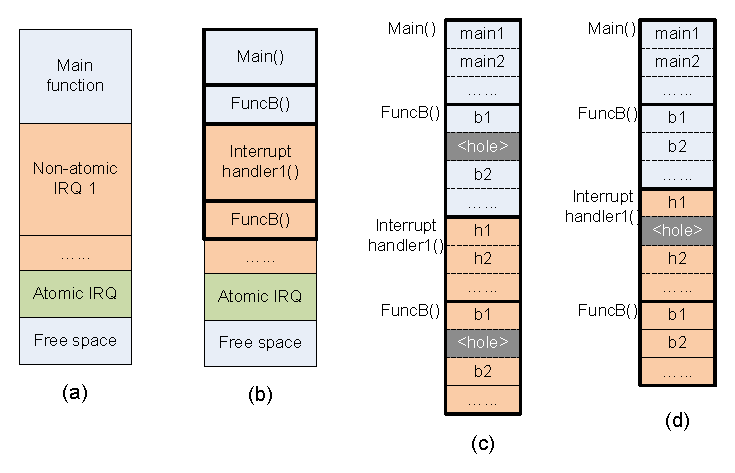
\includegraphics[width=4.5in]{figures/stack.eps}
\caption{An example of data allocation for general purpose applications.}
\label{stack}
\end{figure*}
Figure~\ref{stack} shows a memory usage example. 
$FuncB()$ is called by both $Main()$ and $Interrupt\_handler1()$, so
it has two instances on the stack, while the other functions only
have one instance. Wasting one word in $FuncB()$ will cause two word
waste in RAM, while wasting one word in $Interrupt\_handler1()$ will
cause only one word waste in RAM. Thus, in order to save RAM usage, we should
move the last variable of function $FuncB()$ instead of $Interrupt\_handler1()$.


%As shown in Figure~\ref{fdata.0}, such a move will cause
%changes in all the instructions that use the last variable. If
%equation (~\ref{spacet}) cannot be satisfied for all the procedures, to keep
%the changes minimum, we should first serve those that might demand the
%most runtime memory but have the least number of uses.  That is, we
%should find a procedure $j$ such that

With such consideration, the function $j$ that we pick should satisfy the following
formular.
\begin{small}
\begin{eqnarray}
{{NumOfInsts_j}\over{Usage_j(last)}} = MAX( {{NumOfInsts_j}\over{Usage_i(last)}} )~~~ {(\forall j, ExtraSpaceSize_j>0)}
\label{factor}
\end{eqnarray}
\end{small}

After we decide which function we will pick, we then relocate the last 
variable in procedure $j$ to one
deleted memory word. By doing so, we can shrink the maximal runtime
memory usage by $NumOfInsts_j$ (as it is the last variable in that
procedure), and incur less code changes (as the variable with less
usage is selected). We then decrement $ExtraSpaceSize_j$ and continue this step
until equation (\ref{spacet}) is satisfied.

For example in Figure \ref{fdata.0}, if {\it d} is not introduced, we
will reuse {\it a}'s space with {\it c} if $SpaceT=0$, i.e. no wasted
space. This will result in two updated instructions related to
 {\it c} and {\it d} respectively. This code still outperforms
the default scheme in Figure \ref{fdata.0}(b) which requires three
instruction updates.

%The data allocation problem may become more complicated if it is
%coupled with code generation where data offset are encoded with
%instruction types. For example successive instructions using
%post-increment addressing (PIA) mode will access successive data in
%memory with implicit address increment between two instructions. If
%data is relocated, new instructions must be inserted to change the
%memory access address in the next instruction.  Fortunately, we
%experimented with {\tt gcc 3.4.3} compiler and found that the PIA mode
%is mainly used to access the four bytes of an integer variable and
%thus is insensitive to the variable relocation. For this reason, we do
%not consider the impact the PIA mode when relocating the data. If they
%are used beyond a word boundary, we treat them individually by
%inserting new addressing instructions.


\subsection{UCC register allocation (UCC-RA) for general purpose applications}
Besides the data allocation results, the register allocation results can also 
affect the similarity between generated binary images.
Instructions need to be updated if the assigned registers are changed.
Thus, another task of UCC is to produce similar register assignment
when generating the new binary.

\subsubsection{Register allocation problem for general purpose applications} 
%

Figure~\ref{freg0} illustrates why different register
allocation decisions can greatly impact the code similarity, and therefore the
update cost. In this example, two variables {\it a} and {\it b}
initially have disjoint live ranges and can be allocated to the same
register {\it R1} (Figure~\ref{freg0}(a)). Assume a small code change
extends {\it b}'s live range into {\it a}'s. If there are enough free
registers, a modern register allocator will assign different registers
to them, as depicted in Figure~\ref{freg0}(b).  Variable {\it b} is
assigned to a new register {\it R2}, resulting in a name change for
all the uses in subsequent statements in the statement range \{5,15\}.
In contrast, an alternative {\em update-conscious} decision may
allocate {\it b} to {\it R2} only for the range \{5,11\} where {\it
R1} is not free, and match the old allocation for the range \{12, 15\}
with one extra {\it mov} instruction, as shown in Figure~\ref{freg0}(c). By comparing these two solutions, it is clear that
while the solution (b) achieves better code quality, the solution (c)
results in less update cost. The discrepancy in energy consumption
between data transmission and instruction execution makes the solution
(c) more appealing as it consumes less energy unless the code is very
frequently executed, or the update is extremely rare.

\begin{figure}
\centering
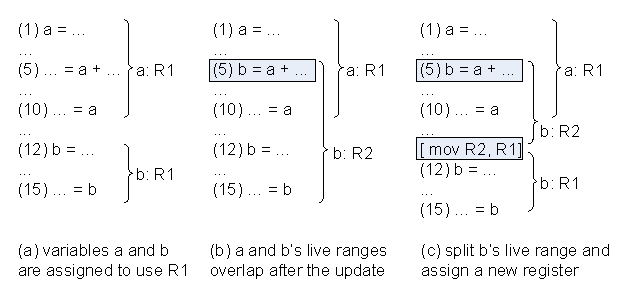
\includegraphics[scale=1.2]{figures/freg.0.eps}
\caption[An example of register allocation for general purpose applications.]{An example of register allocation for general purpose applications.
(a). Variable {\it a} and {\it b} are assigned with register {\it R1};
(b). The live ranges of {\it a} and {\it b} overlap with each other after the code update;
(c). Split {\it b}'s live range and assign a new register to it.}
\label{freg0}
\end{figure}


\subsubsection{UCC register allocation for general purpose applications}\label{secra}
%

The basic idea of UCC register allocation (UCC-RA)~\cite{ucc} is to retain mostly the old register assignments and perform new register allocations to the changed and new instructions {\em with preferences to the decisions for the given binary}. 

To achieve this, IR instructions are first identified as ``changed'' or ``non-changed'', and then successive instructions of the same type are grouped into chunks. The register allocator then allocates registers for each chunk.
Decisions for ``changed'' chunks are made by UCC-RA, while decisions for ``unchanged'' chunks are taken from the old code before the update. For the variables whose live ranges span across the chunk boundary, the register allocation consistency is checked at the end. Inter-register movement instructions may be added to ensure the the semantic correctness.

While doing UCC-RA, each variable in the input chunk is tagged with the register name that was assigned in the old binary. This tag is called {\em preferred-register tag}. The {\em preferred-register tag} is a hint to improving code similarity in UCC-RA.

The register allocator then allocates registers for each changed chunk, and gradually matches the register assignment, or allocation decisions from both changed and non-changed chunks for semantic correctness. Decisions for changed chunks are made by our UCC-RA while decisions for unchanged chunks are taken from the old code before the update. The two decisions are made conjointly. If a variable's live range spans across the chunk boundary, from ``changed'' to ``non-changed'' or vice versa, then the assignment in the ``changed'' chunk gives {\em preference} to the assignment in the ``non-changed'' chunk to maximize the similarity. However, this preference may not always be adopted by the allocator. If the allocator decides to use a new register in the ``changed'' chunk, then a {\tt mov} instruction between the two chunks should be inserted to move data between the new and the old registers. Register preference should also be given to the same variables on different control flow paths (they might be of different chunk types). However, if the allocator chooses a different register, then a {\it mov} instruction is also necessary.

Clearly, placing too many inter-register movement instructions requires not only transmitting more update data to remote sensors but also executing more instructions at runtime. Therefore, it is desirable to develop a precise cost-benefit model such that an inter-register movement instruction is inserted only if it is estimated to be energy-efficient.

\paragraph{Formalizing the UCC register allocation}
Motivated by the 0/1 integer linear programming research for register allocation \cite{related:ilp}, the UCC-RA problem can be formulated as a non-linear integer programming problem. The general idea of how to select the decision variables, formulate the constraints and the objective function is addressed the below. 

\textbf{The decision variables.} 
I use a set of decision variables that represent the register assignments we need to make at each program point. The decision variable is defined as~\ref{decision_vars}. 

\begin{small}
\begin{eqnarray}
X_{op.v.s}^{Ri} = \left\{\begin{array}{r@{\quad:\quad}l}
0  & \mbox{Assertion is true.}\\
1  & \mbox{Assertion is false.}
\label{decision_vars}
\end{array}\right.    
\end{eqnarray}

\begin{center}
\begin{tabular}{c|p{2.0in}} 
$op$ & operation;\\
$v$ &  variable;\\
$s$ & statement; \\
\end{tabular}
\end{center}
\end{small}

The decision variables $X_{op.v.s}^{Ri}$ can be 0 or 1.
With the value assigned to be 1, it means that register {\it Ri} is assigned to variable {\it v} at statement {\it s} for operation {\it op}, and 0 otherwise. For example, when decision variable $X_{def.v.s}^{Ri}$ is set to 1, it means that the variable {\it v} is defined at statement {\it s}, and  register {\it Ri} is assigned to hold the value of variable {\it v}. 
In the example shown in Figure~\ref{freg0}(b) statement (1), the decision variable that is used to determine whether
to allocate variable {\it a} in {\it R1} can be written as $X_{def.a.1}^{R1}$.
\textbf{The objective function.}
Let us use a simple example in Figure \ref{freg0} to explain the proposed procedure. The code contains several instructions: the first two are the definitions of variable {\it a} and {\it b} respectively, while the third one uses both variables. Let us assume at statement (6), {\it a} is dead but {\it b} is still alive, and the preferred-registers of {\it a} and {\it b} are {\it R1} and {\it R2} respectively.

\begin{figure}[htbp]
\begin{tabular}{c|p{5.0in}} 
$a / s / Ri$  & variable {\it a} / statement {\it s} / Register {\it Ri} (1$\le$i$\le$31); \\
~\\

$X_{mov.out.a.s}^{Ri}$ & if {\it a} is moved from {\it Ri}
to another register at {\it s}; \\

$X_{mov.in.a.s}^{Ri}$ & if {\it a} is moved from another
register to {\it Ri} at {\it s}; \\

~ \\

$X_{def.a.s}^{Ri}$ & if {\it a} is allocated to {\it Ri} at its
definition point {\it s};\\

$X_{cont.a.s}^{Ri}$ & if {\it a} is allocated to {\it Ri} after its
def point {\it s}; \\

$X_{lastUse.a.s}^{Ri}$ & if {\it a} is allocated to {\it Ri} at its
last use point {\it s} and {\it a} is dead after {\it s}. \\

$X_{use.a.s}^{Ri}$ & if {\it a} is allocated to {\it Ri} at {\it s},
but not in {\it Ri} after {\it s}; statement {\it s} is not the last
use.\\

$X_{useCont.a.s}^{Ri}$ & if {\it a} is allocated to {\it Ri} at {\it
s}, and is also in {\it Ri} after {\it s}; statement {\it s} is not
the last use.\\

~ \\

$X_{st.a.s}^{Ri}$ & if {\it a} is spilled from {\it Ri} to memory
after {\it s};\\

$X_{ld.a.s}^{Ri}$ & if {\it a} is loaded from memory to {\it Ri}
before its use point {\it s}; \\

$X_{cont.a.s}^{mem}$ & if the variable is kept in memory after the
statement {\it s};
\end{tabular}
\caption{The decision variables used in UCC-RA.}
\label{decisionvars}
\end{figure}

For the code chunk in Figure \ref{freg0}(a), we first introduce a set
of decision variables that represent the register assignments we need
to make at each program point. For example, If variable {\it a} is allocated in
register {\it R1} at statement (1), then we have $X_{def.a.1}^{R1}=1$
and $\forall Ri, Ri\neq R1, X_{def.a.1}^{Ri}=0$. Here
$X_{def.a.s}^{Ri}$ is a decision variable to show if variable {\it a}
is assigned to the register {\it Ri} at statement {\it s}. 
As another example,
if we decided to insert an instruction ``{\it mov R2 to R3}'' for {\it
b} before statement (4), we set $ X_{mov.out.b.4}^{R2}=1$,
$X_{mov.in.b.4}^{R3}=1,$ and all other {\it mov} decision variables
$X_{mov.*.b.4}^{*}$ as 0. As discussed, such a {\it mov}
instruction may be inserted to release {\it R2} for other variables,
or to match the old assignment of {\it b} to {\it R3} after statement
(4).  Figure~\ref{decisionvars} shows a full list of decision variables that we used in
UCC-RA.


When defining proper decision variables, we aim to keep the total
number small so that the solver takes less time to find a
solution. For example, we introduce two decision variables
$X_{mov.in.a.s}^{Ri}$ and $X_{mov.out.a.s}^{Ri}$ instead of a more
intuitive $X_{mov.a.s}^{Ri\leftarrow Rj}$ (move {\it a} from {\it Rj}
to {\it Ri} at statement {\it s}) because of the following reason.
Assume there are 31 registers; the one-variable definition would
introduce $31\times30$ {\em mov} decision variables for each variable
at a program point. This will increase the problem size and slow down
the solver. Instead, we decouple the {\it mov}'s source register from
the destination register such that only $31\times 2$ decision
variables are required. Then, we simply combine the
corresponding move-in and mov-out variables to implement the register
move.

\textbf{The constraints.} 
With the defined decision variables, we convert the register allocation
problem into a problem of finding the 0/1 solution to these
variables. To ensure that the value assignment can be mapped back to a
valid register assignment, these variables are subject to a set of
constraints.

We first define the constraints for variable definitions.  Each
variable should be allocated to one and only one register at its
definition point. Thus, we have, for each variable {\it a} at its
definition point {\it s}, one and only one $X_{def.a.s}^{Ri}$ can be
1, or,

\begin{small}
\begin{eqnarray}
\sum_{\forall Ri} X_{def.a.s}^{Ri} = 1.
\end{eqnarray}
\end{small}

To ensure valid inter-register movements, we define constraints on
{\it mov} decision variables as well. Since we may and may not insert
a move instruction at a program point; and the move-in and move-out
decision variables should appear in pairs, we have:

\begin{small}
\begin{eqnarray}
\sum_{\forall Ri} X_{mov.out.a.s}^{Ri} \leq 1  \nonumber \\
\sum_{\forall Ri} X_{mov.out.a.s}^{Ri} = \sum_{\forall Ri} X_{mov.in.a.s}^{Ri}
\end{eqnarray}
\end{small}

At a statement {\it s}, variable {\it a} may be loaded from the
memory, or come from inter-register movement. After defining the
variable, the value in the register may be spilled to the memory, or
moved to another register, or stay for later use. Thus we have:

\begin{small}
\begin{eqnarray}
X_{st.a.s}^{Ri} \leq X_{def.a.s}^{Ri} + X_{mov.in.a.s}^{Ri} \nonumber \\
X_{mov.out.a.s}^{Ri} \leq X_{def.a.s}^{Ri}  \nonumber \\
X_{cont.a.s}^{Ri} \leq X_{def.a.s}^{Ri} + X_{mov.in.a.s}^{Ri} 
\end{eqnarray}
\end{small}

For the code spill at a definition point, only a store instruction may
be possibly generated. Thus, we have:

\begin{small}
\begin{eqnarray}
X_{cont.a.s}^{mem} \leq \sum_{\forall Ri}X_{st.a.s}^{Ri}
\end{eqnarray}
\end{small}

We next define the constraints for variable uses. Since we can know if
a use is the last use (through backward analysis),
$X_{lastUse.a.s}^{Ri}$ is always exclusive from
$(X_{use.a.s}^{Ri}+X_{useCont.a.s}^{Ri})$. In addition,
$X_{use.a.s}^{Ri}$ and $X_{useCont.a.s}^{Ri}$ are exclusive, and a use
should be in a register. The above are specified as:

\begin{small}
\begin{eqnarray}
\sum_{\forall Ri} X_{lastUse.a.s}^{Ri} = 1;  ~~~~or \nonumber \\
\sum_{\forall Ri} (X_{use.a.s}^{Ri} + X_{useCont.a.s}^{Ri}) = 1;
\end{eqnarray}
\end{small}

At a use point, a variable may be located in a register due to its use in the
previous instruction, or loaded from the memory, or moved
from another register. Depending on whether it is the last use, we
have one of the following two constraints:

\begin{small}
\begin{eqnarray}
X_{use.a.s}^{Ri} + X_{useCont.a.s}^{Ri} \leq X_{cont.a.{\bf(s-1)}}^{Ri} + X_{ld.a.s}^{Ri} + X_{mov.in.a.s}^{Ri} \nonumber 
\end{eqnarray}
\end{small}
\vspace{-0.1in}
\begin{small}
\begin{eqnarray}X_{last.a.s}^{Ri} \leq X_{cont.a.{\bf(s-1)}}^{Ri} + X_{ld.a.s}^{Ri} + X_{mov.in.a.s}^{Ri} 
\end{eqnarray}
\end{small}

Since we only generate load spill, or inter-register movement
before the use point, we have:

\begin{small}
\begin{eqnarray}
\sum_{\forall Ri}X_{ld.a.s}^{Ri} \leq X_{cont.a.{\bf(s-1)}}^{mem} \nonumber \\
\sum_{\forall Ri}X_{mov.out.a.s}^{Ri} \leq X_{cont.a.{\bf(s-1)}}^{Ri}
\end{eqnarray}
\end{small}

The following constraints are used to ensure that one register is assigned to
only one variable at a time.

$U_{a.s}$ is defined to describe the register assignment to the variable {\it a}
at instruction {\it s}.

\begin{small}
\begin{eqnarray}
U_{a.s} = \left\{\begin{array}{r@{\quad:\quad}l} 
X_{def.a.s}^{Ri} & \mbox{if {\it a} is defined at {\it s}} \\ 
X_{use.a.s}^{Ri} + X_{useCont.a.s}^{Ri} & \mbox{if {\it a} is used at {\it s}} \\
X_{lastUse.a.s}^{Ri} & \mbox{if {\it a} is used at {\it s} and no longer used in the later instructions}\end{array}\right. 
\end{eqnarray}
\end{small}

$V_{a.last\_s}$ is defined to show the register assignment information of the last access
point of variable {\it a}. 
Depending on whether instruction {\it last\_s} is a defintion point or use point of variable {\it a}, 
$V_{a.last\_s}$ is calculated in two different ways.

\begin{small}
\begin{eqnarray}
V_{a.last\_s} = \left\{\begin{array}{r@{\quad:\quad}l} 
X_{cont.a.last\_s}^{Ri} & \mbox{if {\it a} is defined at {\it last\_s}} \\ 
X_{useCont.a.last\_s}^{Ri} &\mbox{if {\it a} is used at {\it last\_s}} \end{array}\right. 
\end{eqnarray}
\end{small}

To make sure that there is no register assignment conflict between the current
variable and the active variables which are processed before, the following constraint
is applied:

\begin{small}
\begin{eqnarray}
\sum_{\forall var}V_{var.last\_s} + U_{a.s} \leq 1 
\end{eqnarray}
\end{small}

For example, the following equations show the constraints at statement (2) in
Figure \ref{freg0}:
\begin{small}
\begin{eqnarray}
U_{b.2} = X_{def.b.2}^{Ri}\nonumber\\
V_{a.last\_use} = X_{cont.a.1}^{Ri}\nonumber \\
thus, ~~X_{def.b.2}^{Ri} + X_{cont.a.1}^{Ri} \leq 1
\end{eqnarray}
\end{small}

Also in order to avoid the register assignment conflict between the variables which
are used in the same instruction, the following constraint needs to be applied:
\begin{small}
\begin{eqnarray}
\sum_{\forall var}U_{var.s} \leq 1 
\end{eqnarray}
\end{small}

For example, the following constraints at statement (6) in Figure \ref{freg0}:

\begin{small}
\begin{eqnarray}
U_{a.6} = X_{lastUse.a.6}^{Ri}\nonumber\\
U_{b.6} = X_{use.b.6}^{Ri} + X_{useCont.b.6}^{Ri} \nonumber\\
thus, ~~X_{lastUse.a.6}^{Ri} + X_{use.b.6}^{Ri} + X_{useCont.b.6}^{Ri} \leq 1
\end{eqnarray}
\end{small}

For Mica2 micro controllers, we need to enforce another type of
constraint. Each register in Mica2 has 8 bits, i.e. one byte. A
32-bit integer variable should be allocated to four {\em
consecutive} registers, i.e., byte {\it a}, {\it a}+1, {\it a}+2, and
{\it a}+3 should be in register {\it Ri}, {\it Ri}+1, {\it Ri}+2, and {\it
Ri}+3 respectively:

\begin{small}
\begin{eqnarray}
X_{use.(a).s}^{Ri} = X_{use.(a+1).s}^{R_{i+1}} \nonumber \\
X_{use.(a+1).s}^{Ri} = X_{use.(a+2).s}^{R_{i+1}} \nonumber \\
X_{use.(a+2).s}^{Ri} = X_{use.(a+3).s}^{R_{i+1}} 
\end{eqnarray} 
\end{small}

At the boundary of changed and unchanged code chunks, and at the merge
point of control flows, we insert inter-register move instructions to
make sure that the values are in proper registers before their next
uses. In our future work, instead of performing inter-register
movements, we will introduce constraints similar to those in
\cite{related:ilp} for the merge point of control flows.




\textbf{The objective function.}
The goal of our integer programming is to minimize the objective
function on total energy consumption, as expressed in equation (\ref{totalE}) in
Figure~\ref{feqn}. The equation defines the total energy consumption of the
changed IR chunk under different register allocation decisions. The notations
used in equation ({\ref{totalE}}) are listed below.
Other terms are explained as follows.
\vspace{-0.1in}
\begin{figure*}[htbp]
\begin{small}
\begin{eqnarray}
E_{total} = 
chg(s) \times E_{changed\_IR} + (1-chg(s))\times E_{unchanged\_IR} +
E_{spill} + E_{extra}  \label{totalE}
\end{eqnarray}
where
\vspace{-0.3in}
\begin{eqnarray}
E_{changed\_IR} &= &\sum_{\forall s} (freq(s) \times E_{exe}) +
\sum_{\forall s}(E_{trans})  \label{cE}\\
%
E_{unchanged\_IR} &= & \sum_{\forall s} (freq(s) \times E_{exe}) + \nonumber\\ 
									&  & \sum_{\forall s}(1-\prod_{\forall a}{X_{def/use.a.s}^{prefer(a,s)}}) \times 					E_{trans} \label{uE}\\
%
E_{spill} &=& \sum_{\forall s, a, Ri}
(freq(s) \times (X_{st.a.s}^{Ri}+X_{ld.a.s}^{Ri}) \times E_{exe}) + \nonumber\\
					& & \sum_{\forall s, a, Ri}( (1-spill(a,Ri,s)) \times
 (X_{ld.a.s}^{Ri}+X_{st.a.s}^{Ri}) \times E_{trans})  \\
E_{extra} &=& \sum_{\forall s, a, Ri}
(freq(s) \times X_{mov.in.a.s}^{Ri} \times E_{exe}) + \nonumber\\
					& &\sum_{\forall a, s, Ri} (X_{mov.in.a.s}^{Ri} \times E_{trans}) 
\end{eqnarray}
\end{small}
\vspace{-0.5in}
\caption{The objective function used in UCC-RA.}
\label{feqn}
\end{figure*}


\begin{figure}[htbp]
\begin{normalsize}
\begin{center}
\begin{tabular}{r|p{5in}} 
$E_{trans}$ & the energy consumed to disseminate one instruction in WSN; \\
$E_{exe}$ & the energy consumed to execute one instruction.
We use the averaged number here and differentiate the memory access 
(load,store) and ALU instructions in the implementation. \\
~ & \\
$prefer(a, s)$ & the preferred-register for variable {\it a} at statement {\it s}; \\
$freq(s)$ & the execution frequency counter of statement {\it s}; \\
~ & \\
$chg(s)$ & if {\it s} is an unchanged IR instruction.
chg(s)=1 if {\it s} has been changed; =0 otherwise;\\
$spill(a, Ri, s)$ & if variable {\it a} was spilled to {\it Ri}/loaded back from {\it Ri} 
at statement s in the old binary; 
\end{tabular}
\caption{The notations used in the UCC-RA objective function.}
\label{notation.obj}
\end{center}
\end{normalsize}
\end{figure}



$E_{spill}$ specifies the energy consumption due to code spill. It
includes two components: the execution energy and the dissemination
energy. The former has to do with the code quality which is the main
goal of many existing allocators. The latter is not negligible when a
new spill is generated or an old spill is removed. It is zero for all
other cases, i.e. either (1-$spill(a,Ri,s)$)=0 or
$(X_{ld.a.s}^{Ri}+X_{st.a.s}^{Ri})=0$ in the equation (13).  For
example, if {\it a} is spilled to {\it R1} in both new and old
binaries, then we have zero transmission cost:

\vspace{+0.1in}
\begin{tabular}{l}
for R1, 1-spill(a,R1,s)=0, $X_{ld.a.s}^{R1}+X_{st.a.s}^{R1}$=1\\ for
Ri(Ri$\neq$R1), 1-spill(a,Ri,s)=1,$X_{ld.a.s}^{Ri}+X_{st.a.s}^{Ri}$=0
\\
\end{tabular}
\vspace{+0.1in}

$E_{changed\_IR}$ specifies the energy consumption due to changed IR
instructions. It includes both the execution and the dissemination
energy consumption as well. As we can see, no matter which register
allocator is used, a changed IR instruction always results in a binary
instruction that should be disseminated to remote sensors. Therefore
$E_{changed\_IR}$ is a constant in the model.

$E_{unchanged\_IR}$ specifies the energy consumption due to unchanged
IR instructions. Assume we have an unchanged IR instruction ``{\it
a=a+b}'' and {\it a} and {\it b}'s preferred-registers are {\it R1}
and {\it R2} respectively. If the new allocation decision follows the
old allocation scheme, then there is no dissemination cost, i.e. the
same binary instruction ``{\it add R1, R2}'' is generated. If {\it a}
is assigned to a different register, say {\it R3}, and we generate
``{\it add R3, R2}'', then this new instruction needs to be
disseminated to replace the old one on the sensor. As shown in
equation (12), this component is non-linear -- one $E_{trans}$ is
introduced for either one or two changes of the two preferred
registers.

$E_{extra}$ is the extra energy consumption due to inserted
inter-register movements. This term is zero if a traditional compiler
decision is used. Our UCC-RA targets at achieving overall energy efficiency,
i.e. $E_{extra}$ is positive only when we can gain more reduction from
other components, e.g. $E_{unchanged\_IR}$.

In the above model, $X_{*}^{*}$ are decision variables that need to be
determined by the UCC-RA, while others such as $chg(s), freq(s),$
etc.  are known for a given code chunk.  Since equation (12) is
non-linear, the above formulation of UCC-RA results in a mixed integer
non-linear programming problem (MINLP) \cite{bonmin}.  While the speed
of MINLP solvers has been improved greatly in recent years
\cite{bonmin}, it is still much slower than solving a linear problem.  Our
experiments results show that MINLP can be orders of magnitude slower
than a linear problem of similar sizes, i.e., similar number of
decision variables and constraint. We next discuss how to convert the
MINLP problem to an ILP problem through approximation.

\textbf{Solve an ILP problem.}
In this section we model the update energy consumption
linearly such that the UCC-RA can be solved using an ILP
solver. 

For an unchanged IR instruction with two variables {\it a} and {\it b}
(to comply with Mica2 AVR ISA, each IR instruction in our model has at
most two different operands). Assume their preferred registers are
{\it R1} and {\it R2} respectively, we can  model the energy consumption as

\begin{small}
\begin{equation}
\sum_{\forall s}(1-X_{use.a...}^{R1} + 
1-X_{use.b...}^{R2})  \times E_{trans} \times \delta 
\end{equation}
\end{small}
\noindent

where $\delta=3/4$, a coefficient that approximates the update cost.
It is decided as follows. Assume each variable has equal opportunity
of being assigned and not assigned to its preferred register. For the
instruction with two variables {\it a} and {\it b} and preferred
registers {\it R1} and {\it R2} respectively, there are four
possibilities altogether: 
\begin{itemize}
	\item {\it a} is in {\it R1}, {\it b} is in {\it R2}; 
	\item {\it a} is in {\it R1}, {\it b} is not in {\it R2};
	\item {\it a} is not in {\it R1}, {\it b} is in {\it R2}; 
	\item {\it a} is not in {\it R1}, {\it b} is not in {\it R2}. 
\end{itemize}
It is clear that case
(i) has no update cost while each of other three cases needs to update
one instruction. Therefore the averaged update cost is $
(3/4)~\times~Cost_{single}$, which decides $\delta$ to be $3/4$.

After converting the model into an ILP problem, I adopt a widely used
ILP solver --- LP\_solve \cite{lpsolve} to find the optimal assignment
of decision variables such that the cost (modeled in the objective
cost function) is minimized.  We can then map decision variables back to
register assignments, and generate the code and the corresponding
update script as well.

\subsection{Integration of UCC-DA and UCC-RA}\label{integration}

When constructing the objective function of the update-conscious register allocation scheme (UCC-RA),
the changed and unchanged IR statements are treated differently.
For the changed IR statements, the code update cannot be avoided, thus, using UCC-RA scheme cannot
gain any benefit for this type of statements. On the other hand, for the unchanged IR statements, 
whether to keep the register assignment the same as the old version or not will determine whether
it is necessary to update the generated binary instruction(s).  Notation $chg(s)$ is used to
differentiate these two kinds of IR statements.

With the consideration of the update-conscious data allocation scheme (UCC-DA), we can see that
for the unchanged IR statements, not only the register allocation results but also the data allocation 
results can affect the transmission energy consumption. If the unchanged IR statement is a memory access instruction,
and the memory address of the operand is changed, no matter how the register allocation is done, the
update energy cannot be waived. Thus, the objective function $E_{total}$ for this statement should be
formated using formular~\ref{cE} instead of formula~\ref{uE} in Figure~\ref{feqn}.

Based on this observation, I propose two solutions to integrate UCC-DA and UCC-RA schemes for general purpose
applications below. One is a near-optimal ILP based solution and another one is a light weight heuristic based solution.


\subsubsection{ILP based integration}
In order to integrate the UCC-DA and UCC-RA solutions for general purpose applications,
let us first introduce a new decision variable to describe whether to reallocate a variable
or not, then the related constraints and the revised objective function.


\textbf{Decision variable $X_{a}^{realloc}$.}
I define a new decision variable that determines whether to allocate the variable in 
a different memory slot from the old version. 
The decision variable is written as $X_{a}^{realloc}$, and {\it a} presents the
variable name. If the value is set to ``0'', the data allocation of this variable
keeps the same; otherwise, it is changed.


\textbf{Data allocation related constraints.}
As described in the UCC-DA algorithm~\ref{alg-data}, there are two constraints
for UCC-DA decision variables, and I formulate those constraints using the notations
shown in Figure~\ref{notation3} as below.
\begin{figure}[htbp]
\begin{tabular}{c|p{5.0in}} 
$X_{a}^{realloc}$ & whether to allocate {\it a} in a different memory slot from the old version; \\
$NumOfInsts_i$ & the projected maximal simultaneous instances of procedure $Pi$;\\
%$Usage_i(a)$ & the usage of variable {\it a} in $Pi$;\\
$ExtraSpaceSize_i$& the wasted memory space of procedure $Pi$;\\
$NumOfDelV_i$ & the total number of deleted variables in $Pi$;\\
$NumOfNewV_i$ & the total number of new variables in $Pi$.\\
\end{tabular}
\caption{The notations used in the ILP based UCC integration.}
\label{notation3}
\end{figure}

The total wasted space on the call stack cannot go beyond the threshold $SpaceT$~\ref{spacet}.
This constraint is formulated as equation~\ref{threshold}.
$NumOfDelV_i$ and $NumOfNewV_i$ are the number of variables that are removed and inserted
in procedure $Pi$, so they are constants for each $Pi$.
$NumOfInsts_i$ represents the projected maximal simultaneous instances of procedure $Pi$,
which is also a constant. 
The new variables are firstly used to fill up the holes created by deleting variables.
If there are fewer new variables than deleted variables, the unchanged variables
in this procedure can be reallocated to fill up the memory ``holes''.
The wasted memory space of procedure $Pi$ is presented in equation~\ref{wastes},
which is equal to the number of deleted variables minus the number of new variables,
then minus the number of reallocated variables.

\begin{figure*}[ht]
\begin{small}
\begin{eqnarray}
Extra_i = \left\{\begin{array}{r@{\quad:\quad}l}
0  & \mbox{$DelV_i \leq NewV_i$}\\
DelV_i - NewV_i -{\sum\limits_{\forall a}{X_{a}^{realloc}}}&  \mbox{$DelV_i > NewV_i$}
\end{array}\right.  \label{wastes} \\
\sum_{\forall Pi}{Extra_i\times InstsNum_i } \leq SpaceT\label{threshold}
\end{eqnarray}
\end{small}
\end{figure*}


Another constraint is that it always allocates the last variable in each procedure first until the
space constraint is met. This constraint is formulated as equation~\ref{last}.
\begin{figure*}[ht]
\begin{small}
\begin{eqnarray}
\forall{a,b} \;\; old\_addr(a) \leq old\_addr(b)\Rightarrow  X_{a}^{realloc} \leq X_{b}^{realloc}\label{last}
\end{eqnarray}
\end{small}
%\caption{Data allocation constraints.}
%\label{dataconsts2}
\end{figure*}



\textbf{Integrated objective function.}
The objective function of the UCC-RA problem is formulated as equation~\ref{totalE}.
There are four parts in the objective function.
The energy consumption of the {\it ALU} instructions is formulated as $E_{changed\_IR}$ and $E_{unchanged\_IR}$.
The energy consumption of the {\it spill} instructions is formulated as $E_{spill}$.
The energy consumption of the inserted {\it mov} instructions is formulated as $E_{extra}$.
Because the data allocation result will only affect the transmission energy consumption of the load/store
instructions, only $E_{spill}$ needs to be reformulated.

In the old formular, there were two factors that determine whether the corresponding load/store instruction needs transmission energy
to update the instruction:
whether there was a spill here in the old binary ($spill(a,Ri,s)$), and how the variables are allocated in the registers($X_{ld.a.s}^{Ri}$ and $X_{st.a.s}^{Ri}$).
For the instructions that did not have the register spill in the old binary, the code
update is required, because this load/store instruction is a newly inserted instruction.
Otherwise, the energy consumpiton depends on whether the register allocation results
are the same as the old ones.
In short, only when either variables $X_{ld.a.s}^{Ri}$ or $X_{st.a.s}^{Ri}$ as well as $spill(a,Ri,s)$
are set to be ``1'', the transmission energy can be saved.

Now, besides these factors, whether to reallocate the variable in memory will also
affect the transmission energy.
When the variable is reallocated in memory, which means $X_{a}^{realloc}$
is set to ``1'', the corresponsing load/store instruction needs update
no matter how the other factors are set.
In other words, the instruction update is not necessary, 
only when the following three conditions are all satisified:
\begin{itemize}
	\item $spill(a,Ri,s)$ is set to be ``1'' which means this instruction was a 
{\it spill} instruction in the old binary;
	\item $X_{ld.a.s}^{Ri}$ or $X_{ld.a.s}^{Ri}$ are set to ``1'' which means that the new
register allocation result is the same as the old binary; and
	\item  $X_{a}^{realloc}$
is set to ``0'' which means the variable is not reallocated in memory.
\end{itemize}
Otherwise, this instruction needs to be transmitted.
Thus, the energy consumption of the load/store instructions is then reformulated as equation~\ref{newspill}.

\begin{figure*}[ht]
\begin{small}
\begin{eqnarray}
E_{spill} &=& \sum_{\forall s, a, Ri}
freq(s) \times (X_{st.a.s}^{Ri}+X_{ld.a.s}^{Ri}) \times E_{exe} + \nonumber\\
					& & \sum_{\forall s, a, Ri}(1-spill(a,Ri,s)\times
 (X_{ld.a.s}^{Ri}+X_{st.a.s}^{Ri})\times (1-X_{a}^{realloc}))\times E_{trans} \label{newspill} 
\end{eqnarray}
\end{small}
\caption{The objective function used in the ILP based UCC integration.}
\end{figure*}

As you can see, the energy function $E_{spill}$(~\ref{newspill}) is no longer a linear function
due to the addition of another decision variable $X_{a}^{realloc}$.
In order to reduce the time spent solving the problem, we need to convert
it into a linear function that will give us an approximated result but 
consumes much less time.
Similar as what we did before in subsubsection~\ref{secra}, $E_{spill}$(~\ref{newspill})
can be rewritten as equation~\ref{newspill2}.
\begin{figure*}[ht]
\begin{small}
\begin{eqnarray}
E_{spill} &=& \sum_{\forall s, a, Ri}
freq(s) \times (X_{st.a.s}^{Ri}+X_{ld.a.s}^{Ri}) \times E_{exe} + \nonumber\\
					& & \sum_{\forall s, a, Ri}(1-spill(a,Ri,s)\times
 (X_{ld.a.s}^{Ri}+X_{st.a.s}^{Ri}+1-X_{a}^{realloc})\times \delta )\times E_{trans} \label{newspill2} 
\end{eqnarray}
\end{small}
\caption{The converted objective function used in the ILP based UCC integration.}
\label{newObj2}
\end{figure*}

Here, $\delta$ is an coefficient that approximates the update cost when we 
convert the integer non-linear problem into an integer linear problem.
Same as in subsubsection~\ref{secra}, we set $\delta$ here to be 3/4.


\subsubsection{Heuristic based integration}

The introduction of the memory reallocation decision variable $X_{a}^{realloc}$ will add $N$ 
decision variables to the ILP problem, where $N$ is the number of variables used in the
program. This will increase the complexity of the ILP problem, thus, increase the
compilation time.
Based on this observation, I design another heuristic based integration algorithm, that
does the data allocation and register allocation separately. This scheme will not
affect the complexity of the ILP problem, because no more decision variables will be introduced.
The detailed algorithm is described as below.

Instead of solving both data allocation and register allocation problems simultaneously, 
the compiler will solve them one after another in sequential order. It does UCC-DA first and find out the variables whose 
memory addresses are to be changed. This information is then passed to UCC-RA. The memory access statements that
access these variables will be considered as changed IRs instead of unchanged IRs.

\begin{figure}[htbp]
\begin{normalsize}
\begin{center}
\begin{tabular}{r|p{5in}} 
$datachg(s)$ & if statement $s$ is a memory access statement and the memory address of the operand is changed
from the old version.
\end{tabular}
\caption{ The notation used in the heuristic based UCC integration.}
\label{notation2}
\end{center}
\end{normalsize}
\end{figure}

I introduce another notation $datachg(s)$ shown in Figure ~\ref{notation2} to describe whether the unchanged IR
statement needs update because of data allocation result changes. After the UCC-DA is done, the compiler marks the variables whose memory location are changed. Then, the $datachg(s)$ parameters of those memory access statements that accesses any of these variables will be marked as ``1''. Otherwise, they will be marked as ``0''.


The objective function needs to be changed as shown in Figure~\ref{newObj}. When both $chg(s)$ and $datachg(s)$ are set to ``0'' , the IR statement is treated as an unchanged statement.
\begin{figure*}[ht]
\begin{small}
\begin{eqnarray}
E_{total} = 
chgIR(s) \times E_{changed\_IR} + (1-chgIR(s))\times E_{unchanged\_IR} + \\
E_{spill} + E_{extra} \\
chgIR(s) =1-(1-chg(s))\times(1-datachg(s))
\end{eqnarray}
\end{small}
\caption{The objective function used in the heuristic based integration.}
\label{newObj}
\end{figure*}

The heuristic based solution is easy to implement, however, the result may not be optimal.
While doing UCC-DA, the compiler does not have any information of the UCC-RA result.
It assumes that reallocating a variable in memory will always increase 
code update overhead and makes a local optimal solution yet may not be the global
optimal solution.

For example, assume that we have two data reallocation options. Reallocating variable
{\it a} and {\it b} gives the equal amount memory space usage, but variable {\it a}
is more frequently used than {\it b}. The UCC-DA is more likely to reallocate variable
{\it b} instead of {\it a}, because this decision will cause less code updates.
However, if later the UCC-RA decides to assign another register for {\it a}, then these {\it a} related instructions still 
have to be updated. It is more energy efficient to reallocate variable {\it a} instead
of {\it b} while doing UCC-DA.

For this type of cases, the ILP based solution can produce a near-optimal solution, 
because it solves the UCC-RA and UCC-DA problems at the same time. However, it will
take longer time. This is the tradeoff between the two proposed algorithms.

\section{UCC for DSP applications}

As discussed in Chapter~\ref{chap:related}, with the address generation unit (AGU), DSP instruction set supports the post-incremental, post-decremental, and pre-decremental instructions,  where address calculated can be in parallel with the other operations,
if the next memory location to be accessed is within the auto modify range of the previous access.
Thus, no extra address calculation instruction is needed for these cases.
An optimal data allocation algorithm is desired to allocate the variables accessed sequentially in adjacent memory slots. So that, less instructions are needed to explicitly update the address registers, which will reduce the code size and execution overhead.

Because of such connection between the data allocation and code generation in DSP applications, keeping data allocation similar as the older version will keep the addressing modes similar as the old version,
therefore the generated binary image. Thus, an update-conscious data allocation scheme is desired for DSP application updates.

Besides that, how to assign address registers to the variables can also affect the generated binary similarity.
Keeping the address register allocation result similar as the old version also improves the generated binary similarity, which reduces the patch size.

\begin{figure}[ht]
\begin{center}
\includegraphics[scale=0.5]{figures/csoa.eps}
\caption[An example of data allocation for DSP applications.]{An example of data allocation for DSP applications. 
(a) The IR code; 
(b) The access graph; 
(c) The interference graph; 
(d) The data allocation result.}
\label{csoa}
\end{center}
\vspace{-10mm}
\end{figure}

\subsection{Data allocation problem for DSP applications}

An motivation of the proposed UCC data allocation (UCC-DA) scheme is shown in  Figure~\ref{csoa}. When a DSP application undergoes a small update, the code before and after the change are similar. Update oblivious schemes generate the new memory layout and its corresponding binary code without considering the similarity between different versions. 

However, an UCC-DA algorithm reads in the old access graph and its interfere graph, and strives to generate a new memory layout that minimizes the update script, i.e. the difference between the new and old binaries. A sensor node only needs to download the update script and regenerates the new binary and/or the new memory layout (Figure~\ref{ioverview}) with simple interpretation.

\begin{figure}[ht]
\begin{center}
\includegraphics[scale=0.5]{figures/updcsoa.eps}
\caption[An example for the need of UCC data allocation for DSP applications.]{A motivational example for the need of UCC data allocation for DSP applications.
(a) The C code after a simple update over Figure~\ref{csoa};
(b) The new interference graph;
(c) The new access graph;
(d) The new data allocation using CSOA, showing significantly different layout from the original assignment shown in Figure~\ref{csoa}(d).}
\label{updcsoa}
\end{center}
\vspace{-10mm}
\end{figure}
Figure~\ref{updcsoa} illustrates the data allocation result of the example shown in Figure \ref{csoa} using an UCC-DA algorithm.
Figure~\ref{updcsoa}(a) shows the new code after a simple change of the above example, i.e. the third instruction is changed (in the box). Using the new access graph and interference graphs CSOA generates a very different variable coalescing result (Figure~\ref{updcsoa}(d)). The memory layout difference further translates to selecting different addressing instructions at each memory access (Figure~\ref{recomdiff}). Out of seven instructions to be updated in the old code, four of them are due to the data allocation change.

\begin{figure}[htbp]
\begin{small}
\begin{center}
\begin{tabular}{|c|c||l||l|l||l|l|} \hline\hline
%    &    & \multicolumn{3}{c|}{Addressing Mode} &  \multicolumn{2}{c|}{Code Update}\\ \cline{3-7}
    & Access   & Original      & \multicolumn{2}{l||}{Update-Oblivious} & \multicolumn{2}{l|}{Update-Conscious} \\ \cline{4-7}
    & sequence & code         & code        & update & code         & update \\ \hline \hline
 0  & a        & ~~$\bullet$++  & ~~$\bullet$   & diff**   & ~~$\bullet$++  &        \\ 
 1  & b        & ~~$\bullet$    & ~~$\bullet$   &        & ~~$\bullet$    &        \\
 2  & b        & ~~$\bullet$    & ~~$\bullet$   &        & ~~$\bullet$    &        \\
 3  & c        & ~~$\bullet$-~- & ~~$\bullet$   & diff   & ~~$\bullet$    & diff   \\
 4  & $\rightarrow$ \textcolor{red}{\bf{a*}}
               & ~~$\bullet$++  &               & diff   &                & diff   \\
 5  & c        & ~~$\bullet$-~- & ~~$\bullet$   & diff   & ~~$\bullet$-~- &        \\
 6  & f        & ~~$\bullet$    & ~~$\bullet$   &        & ~~$\bullet$    &        \\
 7  & f        & ~~$\bullet$    & ~~$\bullet$++ & diff**   & ~~$\bullet$    &        \\
 8  & e        & ~~$\bullet$++  & ~~$\bullet$-~-& diff**   & ~~$\bullet$++  &        \\
 9  & c        & ~~$\bullet$-~- & ~~$\bullet$++ & diff**   & ~~$\bullet$-~- &        \\
 10 & e        & ~~$\bullet$    & ~~$\bullet$   &        & ~~$\bullet$    &        \\
 11 & d        & ~~$\bullet$    & ~~$\bullet$   &        & ~~$\bullet$    &        \\ \hline 
\multicolumn{7}{l}{ } \\
\multicolumn{7}{l}{*: This access only exists in the old version.}\\
\multicolumn{7}{l}{**: The instruction that needs to be updated, due to data allocation changes.}\\
\multicolumn{7}{l}{$\bullet$++: An instruction with post-increment addressing.}\\
\multicolumn{7}{l}{$\bullet$-~-: An instruction with post-decrement addressing.}\\
\multicolumn{7}{l}{The old version memory layout is ~~``slot 0: a, d, e, f; slot 1: b, c''}\\
\multicolumn{7}{l}{The memory layout for GCC result is ``slot 0: a, b, c, f; slot 1: d, e''.}\\
\multicolumn{7}{l}{The memory layout for UCC result is ``slot 0: a, d, e, f; slot 1: b, c''.}
\end{tabular}
\end{center}
\end{small}
\caption{The update script comparison between CSOA and the update-conscious scheme.}
\vspace{-0.2in}
\label{recomdiff}
\end{figure}





\subsection{UCC data allocation (UCC-DA) for DSP applications}
The design goal of the UCC data allocation is to keep the memory layout similar between the old and new versions.
with minimal run-time performance loss.
In order to solve this problem, a incremental coalescing offset assignment scheme is proposed. This algorithm 
assumes that there is only one address register and solves the data allocation problem
by keeping the data allocation similar as the old data allocation result.


\subsubsection{Incremental coalescing single offset assignment (ICSOA)}


To minimize the update script, I propose to perform update-conscious code updates through incremental coalescing SOA (ICSOA) (Figure~\ref{ioverview}). When a DSP application undergoes a small update, the change does not greatly affect the binary code. On the server side, ICSOA reads in the old access graph and its interference graph, and strives to generate a new memory layout that minimizes the update script. On the mobile system side, only the update script needs to be downloaded. With simple interpretation, the mobile system  regenerates the new binary and/or the new memory layout.

\begin{figure*}[htbp]
\begin{center}
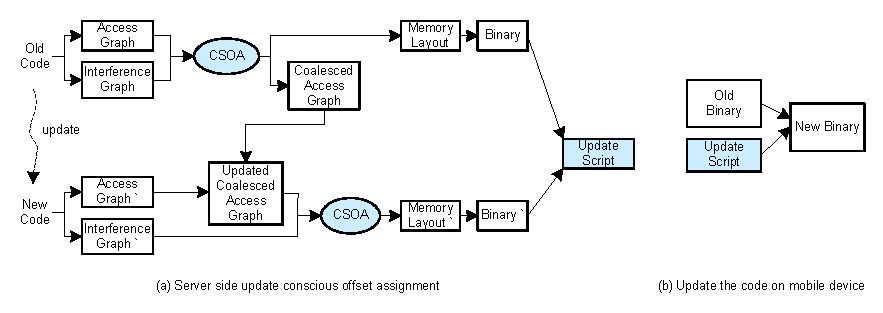
\includegraphics[scale=1.2]{./figures/icsoa-overview.eps}
\caption{An overview of ICSOA-based code update scheme.}
\label{ioverview}
\end{center}
\end{figure*}


The pseudo code of ICSOA is shown in Algorithm \ref{icsoaalg}. It first builds the access graphs before and after the code update, performs the CSOA algorithm, retrieves the coalesced variable assignment in $\textit{CAG}_1$, updates the new access graph $\textit{AG}_2$, resolves possible conflicts when applying the old layout to the new code, and calls CSOA again to find the new offset assignment. 

\begin{algorithm}
\caption{Incremental Coalescing-Based SOA (ICSOA)}
\singlespace
\label{icsoaalg}
\begin{algorithmic}[1]
\singlespace
\REQUIRE $\textit{AS}_1$,$\textit{AS}_2$: access sequences before and after update; \\
				 $\textit{IG}_1$,$\textit{IG}_2$: interference graphs before and after update;
\ENSURE the offset assignment.

\STATE $\textit{AG}_1$ $\leftarrow$ Build access graph using $\textit{AS}_1$;
\STATE $\textit{AG}_2$ $\leftarrow$ Build access graph using $\textit{AS}_2$;

\STATE $\textit{CAG}_1$ $\leftarrow$ CSOA($\textit{AG}_1$,$\textit{IG}_1$); 
\STATE $\textit{AG}_\textit{NEW}$ $\leftarrow$ update\_access\_graph($\textit{CAG}_1$,$\textit{AG}_2$); 
\STATE resolve\_conflicts($\textit{AG}_\textit{NEW},\textit{IG}_2$); 
\STATE $\textit{CAG}_2$ $\leftarrow$ CSOA($\textit{AG}_\textit{NEW}$, $\textit{IG}_2$);
\STATE Return offset assignment based on $\textit{CAG}_2$;
\end{algorithmic}
\end{algorithm}

\paragraph{Function  update\_access\_graph().} It combines the access graph result of the old version ($\textit{CAG}_1$) and the newly generated access graph ($\textit{AG}_2$), into a new access graph ($\textit{AG}_\textit{NEW}$).
We build $\textit{AG}_\textit{NEW}$ based on $\textit{CAG}_1$, by adding new variable nodes and removing unused nodes, so that
$\textit{AG}_\textit{NEW}$ not only represents the updated access sequence but also keeps all the coalescing offset assignment result from the old version.
Using $\textit{AG}_\textit{NEW}$ instead of $\textit{AG}_2$ as the offset assignment input helps to improve the offset assignment similarity with the previous version, and reduces the patch transmission overhead.
However, when the code change is relatively large, the energy saved by improving code similarity may be offset by the code quality loss. 
For this reason, when combining the graphs, {\it update\_access\_graph()} evaluates the number of accesses of each old variable in the new code, and extracts it from its coalesced group if the variable has more new or updated accesses than the unchanged ones. 
The intuition is to extract the variables from their old coalescing groups only if it can bring explicit benefits. 
A new node is introduced for each extracted variable. Empty group nodes will be removed from $\textit{AG}_\textit{NEW}$.
At the end, the function adjusts the weights of impacted access edges accordingly to finish the update.


\paragraph{Function resolve\_conflicts().}In the code update, two variables that were coalesced in the old assignment may interfere with each other. We identify this as a {\em conflict} and use the function {\it resolve\_conflicts()} to resolve it. 

The function first orders the variables in each coalescing group, by the factor 
$$\frac{\textit{Num}_{\textit{local}\_\textit{itfs}}}{\textit{Num}_{\textit{local}\_\textit{acs}}} .$$
Here, $\textit{Num}_{\textit{local}\_\textit{itfs}}$ represents the number of interferences between the variable and the other group members, and $\textit{Num}_{\textit{local}\_\textit{acs}}$ represents the number of adjacent accesses between this variable and the other group members. The function then extracts the interfering variable that has the highest factor value one by one until all the interferences in the group are resolved. By doing so, the variables that create more interferences but have fewer adjacent accesses with the others are extracted earlier from the coalescing group. 

For each variable chosen to be extracted from the coalescing group, the function splits the live range (i.e. conflict range) into to two subranges, the original part and the newly extended part. We use the old variable name to represent the original subrange, and introduce a {\em patch variable} for the extended subrange. To ensure semantic correctness, we insert {\it a'=a} or {\it a=a'} to move the value between the subranges. The insertion involves memory copy and tends to incur large overhead. We will evaluate its impact in the experiments.
 
For the example in Figure~\ref{csoa}, ICSOA combines the coalesced offset assignment (Figure \ref{csoa}(d)) and the new access graph (Figure~\ref{updcsoa}(c)). Figure \ref{icsoa}(a) shows the updated access graph. As there is no conflict between the access graph and interference graph, ICSOA outputs the same coalesced assignment (Figure \ref{icsoa}(c)). In this example, the script generated from ICSOA is 71\% smaller than that of recompilation using CSOA.

\begin{figure}[htbp]
\begin{center}
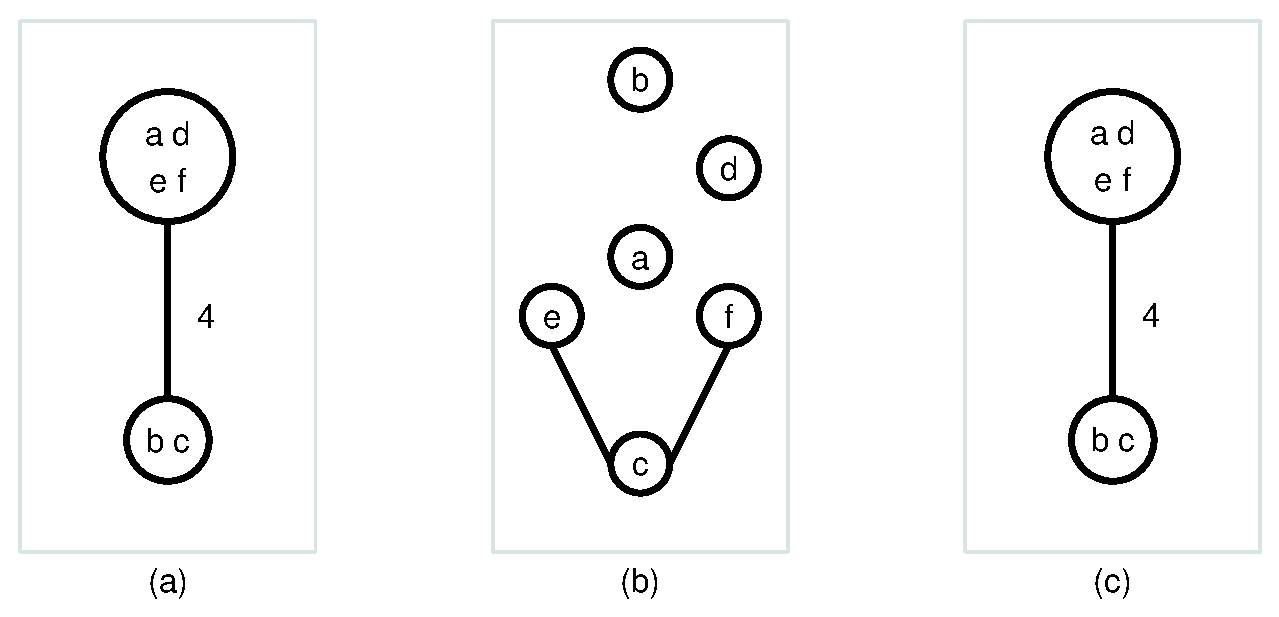
\includegraphics[scale=0.5]{./figures/icsoa.eps}
\caption[An example of ICSOA scheme.]{An example of ICSOA scheme:
(a) $\textit{AG}_\textit{NEW}$, the updated access graph;
(b) $\textit{IG}_2$, the new interference graph;
(c) The final offset assignment.}
\label{icsoa}
\end{center}
\vspace{-0.15in}
\end{figure}

\subsection{Address register allocation and data allocation for DSP applications}
In practice, more address registers are available on DSP chips. Keeping the address register assignment to the variables the same as the old version may also improve the binary level similarity.
I propose an update-conscious address register allocation scheme for DSP applications here that generates a similar association between the address registers and variables
with the old version, and integrate that with the data allocation scheme (ICSOA).

\subsubsection{Incremental coalescing general offset assignment (ICGOA)}
The ICSOA algorithm proposed above solves the data allocation problem for DSP applications when there is only one available address register, while this ICGOA algorithm here is to solve more realistic problems. It is developed based on the CGOA algorithm~\cite{related:ottoni}. The goal is to solve both address register allocation and data allocation problems for DSP applications.

This problem can be formulated as how to divide the variables into a certain number of groups, assuming that accesses to the variables in the same group will use the same address register.
Then we can use the ICSOA algorithm proposed above to allocate the variables in each partition group and generate the complete memory layout by combining the partial data allocation
results. The detailed algorithm is presented in Algorithm~\ref{icgoaalg}. 

\begin{algorithm}[htbp]
\singlespace
\begin{algorithmic}[1]
\singlespace
\REQUIRE $\textit{AS}_1$,$\textit{AS}_2$: access sequences before and after update; \\
				 $\textit{IG}_1$,$\textit{IG}_2$: interference graphs before and after update;\\
				 the number of address registers $N_{AR}$;
\ENSURE the offset assignment.\\
\COMMENT{Run CGOA over the original code}
\STATE $\textit{Partition}_1[N_{AR}] \leftarrow \textit{CGOA}(\textit{AS}_1,\textit{IG}_1,N_{AR})$;\\
\COMMENT{Remove the deleted variables and partition the newly added variables}
\STATE $\textit{Partition}_2[N_{AR}] \leftarrow  \textit{ICGOA}\_\textit{Partition}(\textit{Partition}_1[],N_{AR},\textit{AS}_2,\textit{IG}_2)$;

\COMMENT{Run ICSOA in each variable partition group}
\FOR {$i=0$ to $N_{AR}$}
\STATE $\textit{Offset}[i] \leftarrow ICSOA(\textit{Partition}_2[i],\textit{AS}_1,\textit{AS}_2,\textit{IG}_1,\textit{IG}_2)$;
\ENDFOR

\STATE Return $\textit{Offset}$;
\caption{Incremental coalescing based GOA (ICGOA).}
\label{icgoaalg}
\end{algorithmic}
\end{algorithm}

It first uses the CGOA algorithm~\cite{related:ottoni} to produce the variable partition of the old version based on the old access graph and interference graph using a heuristic based algorithm. 
In this algorithm, the variables are sorted by the decreasing order of the {\it global interference number} $\textit{Num}_{\textit{global}\_\textit{itfs}}$, which is the total number of interferences that each variable has with the other variables. The variable that has a higher {\it global interference number} is processed earlier than the ones with lower {\it global interference numbers}, because they have more constraints.
Then, CGOA determines the partition group that the variable belongs to according to the {\it local interference numbers} $\textit{Num}_{\textit{local}\_\textit{itfs}}$. This number represents the number of interferences that this variable has with the other variables within a partition group. The {\it local interference number} between each variable and each partition group is calculated and the variable is assigned to the group that has the smallest {\it local interference number}.
This partition result is saved in $\textit{Partition}_1$ in algorithm~\ref{icgoaalg}.


Based on the old partition result $\textit{Partition}_1$, the removed variables are first deleted from each partition. New variables are considered next. 
Same as CGOA, the new variables are first ordered by the {\it global interference number}.
Each variable tends to be assigned with the group that has the fewest {\it local interferences}.
This generated new partition $\textit{Partition}_2$ should be very similar as the old one, because it just incorporates the variable changes to the old partition.

After that, we run the ICSOA algorithm within each partition group to generate the memory layout for the variables inside each group.
The ICSOA results are then combined to form the final result.



\chapter{Software differential patching}
With the new binary versions generated by the UCC technique, I define a update script format to summarize the code difference between the base binary and the newly generated binary, transmit the patch script to the sensors, and let the sensors reconstruct the new binary. As shown in Figure~\ref{patch}, the old version binary \texttt{E} and the new version binary \texttt{E'} are first compared, and then the binary level differences are formatted as the update script \texttt{U}. After the sensors receive the complete \texttt{U}, they will retrieve the new binary image \texttt{E'} by combining \texttt{U} with the old binary image \texttt{E} which already exists in the sensor memory.

\begin{figure}[htbp]
\centering
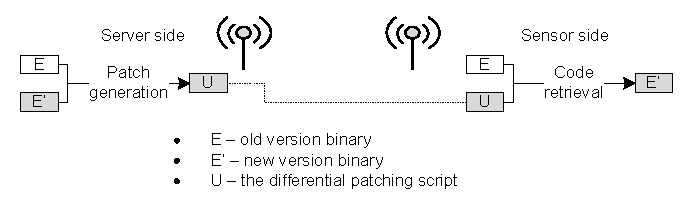
\includegraphics[scale=1.2]{figures/patch.eps}
\caption{Patch generation and binary construction.}
\label{patch}
\end{figure}


The binary code may be changed due to functionality change or data layout change, thus, I separate these two kinds of changes in the update script, as the functionality script part and data layout part representatively.
The design of the script primitives affects both the update data packet transmission effectiveness and the runtime overhead on each sensor node. To facilitate the description of the UCC techniques, I adopted four simple code update primitives, similar to those in prior work~\cite{related:script}, and propose three advanced functional primitives and three data layout primitives to describe the higher level code changes. 

\section {Instruction based patching}

I use the functional binary update primitives to describe the functional changes, such as adding, removing or updating instructions caused by functionality changes. 
I adopted the simple primitives from the prior work~\cite{related:script} and proposed the advanced primitives to solve more complicated code compression problems. The difference between the advanced primitives and the simple primitives is that they are not used to describe the simple bit level comparison results, but higher level structure changes such as the destination address shifting for a group of instructions.

The format of the script primitives is shown in Figure~\ref{fscript}. 

\begin{figure}[htbp]
\centering
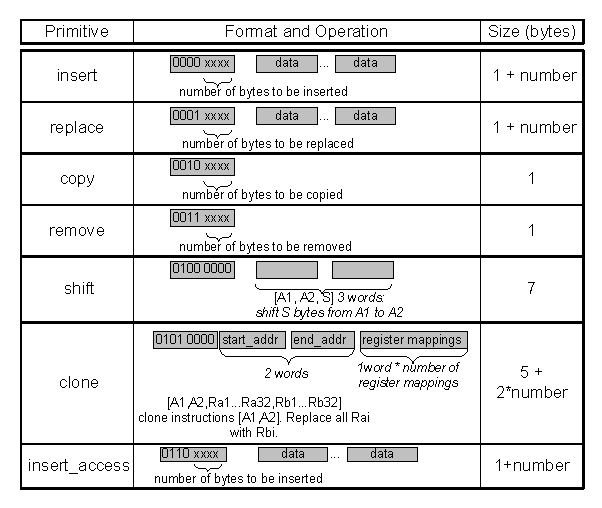
\includegraphics[scale=1.2]{figures/fopcode.eps}
\caption{The patch script primitives -- code part.}
\label{fscript}
\end{figure}


\subsection{Simple primitives}

There are four simple primitives --- {\tt insert}, {\tt replace}, {\tt copy}, and {\tt remove}. Both {\tt insert} and {\tt replace} primitives have one-byte opcode and {\tt n} bytes of data/instructions to be incorporated.  The {\tt copy} and {\tt remove} primitives take one byte each and specify the size of old data/instruction block to be
copied or removed.

\begin{figure}[htbp]
\centering
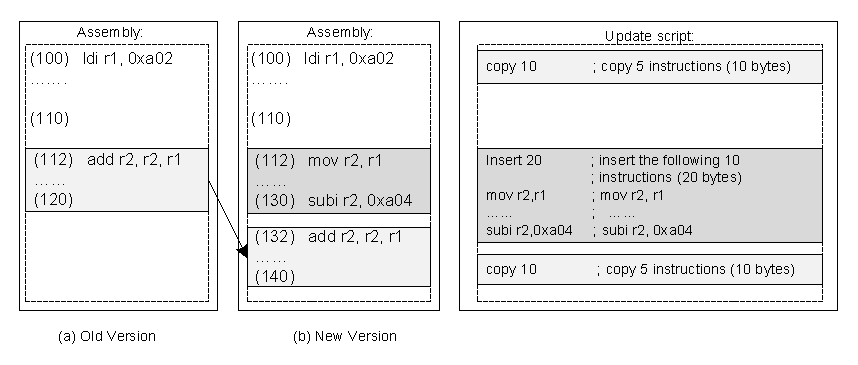
\includegraphics[width=6in]{figures/sother.eps}
\caption{An example of update script involving the simple primitives. 
New code {\tt [112,130]} is inserted.
{\tt [112,120]} in the original code is now moved to {\tt [130,140]} 
in the new version.
}
\label{fsother}
\end{figure}

Figure \ref{fsother} shows a simple example of the simple primitives. The new version contains three chunks of code, {\tt [100,110]}, {\tt [112,130]}, and {\tt [132,140]}. Both the first and third chunks can be found in the old code while the second chunk is new. Therefore the update script contains two {\tt copy} primitives and one {\tt insert} primitive. The {\tt insert} primitive has a one-byte opcode and ten instructions (or 20 bytes). The total size of the update script is 23 bytes.  

In order to interpret the simple primitives on remote sensors,
the script interpreter maintains two instruction pointers, one points to the old
binary image and the other points to the last instruction that has been generated
in the new binary image. 
The {\tt insert} primitive inserts the instructions
in its data part into the new binary image, and moves the pointer in the
new code to the end. The {\tt replace} primitive does the same thing to
the new binary but also moves the pointer in the old binary for the
same distance. The {\tt copy} primitive reads the instructions from the
old binary, and moves both pointers.
 
\subsection {Advanced primitives}
In the experiment, I observed some code structure changes that affect more than one instruction. For example, when the register assignment of one variable is different in the new binary, all the instructions that access this variable need to be updated. Since the affected instructions are usually more than one, it is cheaper to incorporate such register assignment changes in the patch script, other than the binary level differences. Based on this observation, I propose three advanced primitives in my design.

\subsubsection {Shift}
As some code may be inserted into or removed from the base binary in software update, the absolute address of the instructions may be changed in the update. Such change might cause the destination address changes for branch instructions. So I use the {\tt shift} primitive~\cite{related:script} that informs the sensors about the destination address shifts, so that the sensors can incorporate such code changes on side. Instead of explicitly updating all the affected branch instructions using several {\tt update} primitives, now we can use one  {\tt shift} primitive to describes such code changes. Thus, the update script size can be significantly reduced. 

As Figure~\ref{fscript} shows, the {\tt shift} primitive contains a one-byte opcode and another three words to indicate that
the code segment {\tt [A1,A2]} is now moved to {\tt [A1+S,A2+S]}. Thus, all the branch/jump instructions whose destination addresses are in the range {\tt [A1,A2]}, will have the destination addresses shifted by {\tt S} on the sensor side.

%To interpret the {\tt shift} script, the binary rewriter running on the sensor nodes needs to have simple decoding ability --- it picks up each control transfer instruction, checks whether its target address falls in the range that needs to be shifted, and updates them with new addresses.
%For absolute branch instructions, their target addresses can be decoded from the instruction directly; for relative branch instructions, their target addresses can be computed by adding the relative offset to the address of the current instruction.

\begin{figure}[htbp]
\centering
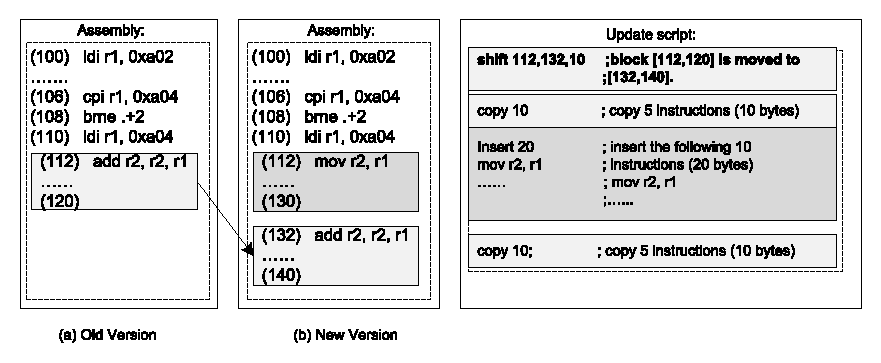
\includegraphics[width=6in]{figures/shift.eps}
\caption{An example of update script involving {\tt shift} primitive. New code {\tt [112,130]} is inserted. {\tt [112,120]} in the old code is now moved to {\tt [132,140]} 
in the new version. Some control flow instructions are affected due to this address change.
}
\label{fshift}
\end{figure}

Figure \ref{fshift} shows an example using the {\tt shift} primitive. Due to the insertion of
new code, the chunk {\tt [112,120]} in the old version is now moved to {\tt [132,140]} 
in the new version. Thus all the control flow instructions that
jump to any instruction in this chunk need to be updated. In the example the {\tt shift} primitive
specifies that all the branch instructions whose targets are in the address range {\tt [112,120]} should be shifted by 20. 

When one block movement causes several changes in the code, using {\tt shift} primitive helps to reduce the script size. The tradeoff is that a slightly more powerful interpreter has to be installed on the sensor side such that it can decode each instruction type to extract the desired target address. 

The sensors will interpret the {\tt shift} primitive in the following way. 
For the absolute branch instructions, the original destination is decoded
first and if it falls in the shift range, it will be updated according
to the offset encoded in the primitive.
For relative branch instructions, their target addresses can be computed by adding the relative offset to the address of the current instruction.

It is implemented by maintaining a shift information table. When encountering a {\tt shift} primitive,
one shift entry is added to the table, which includes the start address, end address and shift offset.
When copying one instruction from the old binary to the new binary, the interpreter will check this table if it is a branch or jump instruction. If the target address falls in any shifting range, the destination of this instruction will be updated.
%\begin{figure}[htbp]
%\begin{center}
%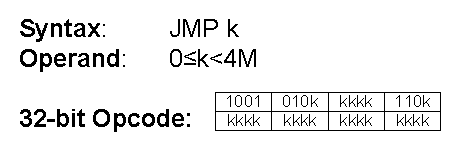
\includegraphics[width=2.2in]{./figures/jump.eps}
%\caption{{\tt JMP} instruction in AVR instruction set.
%}
%\label{jump}
%\end{center}
%\end{figure}
%For example, in the AVR instruction set~\cite{avr-inst}, {\tt JMP} instruction updates the
%the program counter to make the execution ``jump'' to the destination.
%The format is shown in Figure~\ref{jump}. The sample code below shows
%how to update the destination address for {\tt JMP} instructions.
%\begin{algorithmic}
%\singlespace
%\IF {$*(P_{old})$ AND 0xfe0e $\neq$ 0x940c} 
%        \STATE old\_dest = (($*P_{old}$ AND 0x01f0) $\gg$ 3 )+  ($*P_{old}$ AND 0x1);
%        \STATE old\_dest $<$= 16;
%        \STATE old\_dest += $*(P_{old}+1)$;
%        \IF {old\_dest $\in$ {shift range}}
%        
%        	\STATE new\_dest = old\_dest + offset;
%        	\STATE new\_inst = 0x940c;
%       	 	\STATE new\_inst\_high $|$= (new\_dest $\gg$16 ) AND 0x1;
%        	\STATE new\_inst\_high $|$= ((new\_dest $\gg$16) AND 0x3e) $\ll$ 3; 
%        	\STATE new\_inst\_low = (new\_dest AND 0xffff);
%        \ENDIF
%\ENDIF 
%\end{algorithmic}

\subsubsection {Clone}
In the experiment, I find that the binary code of the {\tt inline} functions called at different locations is very similar with each other, except for the register usages. This is because they are compiled from the same source code, however, due to the different context, different register assignment decisions may be made. Thus, they only differ in the register usages.
So when an {\tt inline} function is introduced or updated, such similar code needs to be inserted or updated more than once in the binary.

Based on this observation, I introduced the {\tt clone} primitive. 
When an {\tt inline} function is inserted or modified in the code update, the update script only includes one copy of the binary generated by the {\tt inline} function, and advises the sensors to 
replicate the master copy with register usage replacement while constructing the binary for the other instances of this function.
The example below shows how the {\tt clone} primitive works.
Assume that an {\tt inline}
function is called at multiple places, such as block {\tt [A1,A2]} and {\tt [B1,B2]}. 
The patch generator uses block {\tt [A1,A2]} as the comparison base, 
and tries to match the register allocation between these two blocks. 
Assume the register mapping between them is shown as below, 
$(\tt{R_{a1},R_{a2},...,R_{an})\Rightarrow(R_{b1}^\prime,R_{b2}^\prime,...,R_{bn}^\prime)}$.
Given such information, instead of using a sequence of the simple primitives to describe the
updated/new code of block {\tt [B1,B2]}, we could rather copy instructions from block 
{\tt [A1,A2]}, and slightly change the register
assignments according to the register mapping 
to rebuild block {\tt [B1,B2]}.

As shown in Figure~\ref{fscript},The {\tt clone} primitive has one-byte opcode, and another
several bytes to specify the starting and ending address 
of the code segment where the code would be copied from, and the register mappings.
The primitive length varies according to the register mapping complexity.
Assume there are {\tt N} pairs of register mappings, the {\tt clone} primitive length is
{\tt 5+2*N}. An {\tt inline} function may have multiple instances in the binary image. The 
instance that is stored with the lowest addresses will be considered as the master copy.
The other instances will clone the code from the master copy.


\begin{figure}[htbp]
\centering
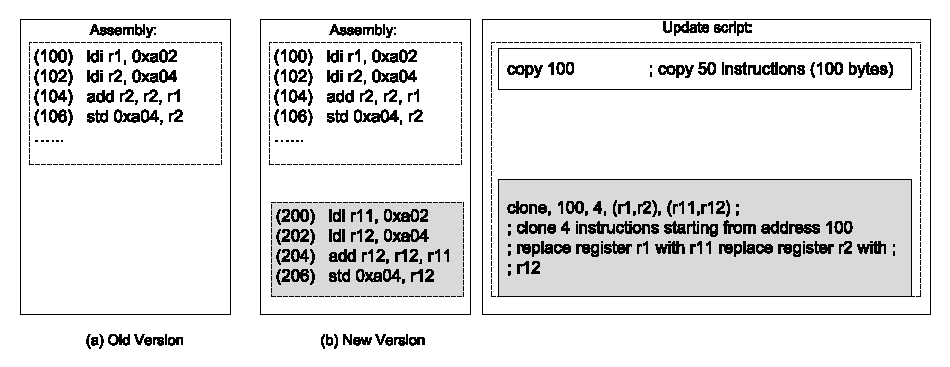
\includegraphics[width=6in]{figures/sclone.eps}
\caption{An example of update script involving {\tt clone} primitive. New code {\tt [200,206]}, which
is compiled from the same {\tt inline} function as code {\tt [100,106]} is inserted.}
\label{fclone}
\end{figure}

Figure \ref{fclone} shows an example using the {\tt clone} primitive.  Both the code {\tt [200,206]} and {\tt [100,106]} are compiled from the same {\tt inline} function. Instead of generating the update script for {\tt [200,206]} by using the {\tt insert} primitive, the {\tt clone} primitive is used to specify that the second code block clones the block {\tt [100,106]} while registers  
${\tt r_1}$ and ${\tt r_2}$ needs to be updated to be ${\tt r_{11}}$ and ${\tt r_{12}}$ respectively.

The {\tt clone} primitive can reduce the script size when the {\tt inline} function is
called at multiple places, and the register mapping is clear. However, if the register mapping
is too complicated the script size could be very big, in which case it is better to use simple primitives, such as {\tt insert} and {\tt replace}. In addition, it requires that the sensor-side interpreter has simple decoding ability to extract register names from different instruction types, and replace them with new ones. 
The sensors need to reconstruct the code segment
by replacing the registers in the master copy according to the patch script.
Each clone operation will need to decode the instructions in the master copy and
replace the registers. Thus, when the master copy is frequently cloned, it is more
efficient to store the master copy in a storage buffer and add tags
to each instruction to indicate whether this is a memory access instruction and
which register is used, so that it can speed up this process.

%In order to interpret the {\tt clone} primitive, the sensor needs to scan the update script twice.
%In the first scan, it builds the clone information table, which includes the start
%and end address of the master copy and the number of clone operations.

%In the second scan, when the new code pointer encounters the master copy, 
%the code segment will be stored in the buffer until all its clone
%operations are complete. The related entry in the clone information table 
%is updated to record the location of the code segment in the buffer.

%When interpreting a {\tt clone} primitive, the
%sensor will look up the clone information table to locate the code segment in
%the buffer, copy it and replace the registers according to the script.
%The clone counter in the information table keeps track of the number of 
%clones that need to be done. Once it reaches zero,
%the buffer used to store the master copy will be released. 
%Figure~\ref{cloneexample} shows the interpretation
%procedure of the example given in Figure~\ref{fclone}.

%\begin{figure}[htbp]
%\centering
%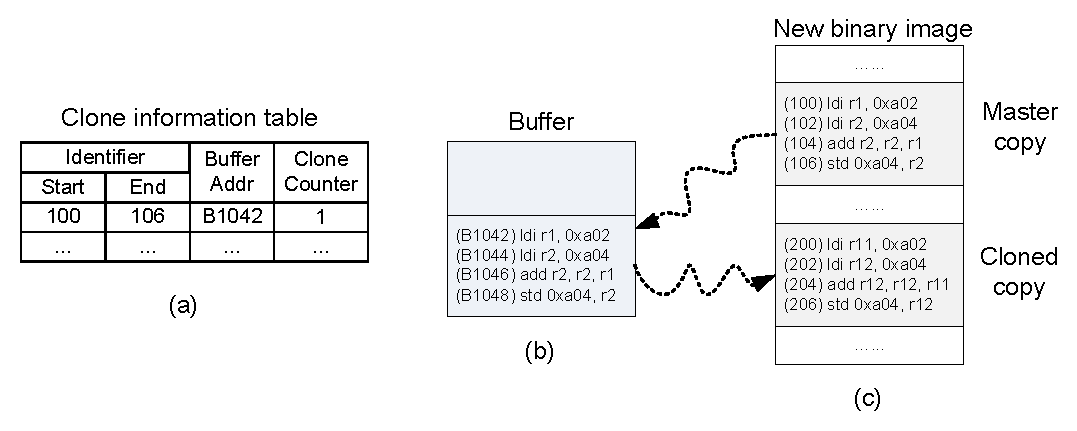
\includegraphics[width=5in]{./figures/clone.eps}
%\caption{An example of the {\tt clone} primitive interpretation procedure.
%(a). The clone information table. (b). The buffer. (c). The 
%reconstructed binary image.}
%\label{cloneexample}
%\end{figure}

%For the frequently cloned master copies, tags can be added to the instructions stored in 
%the buffer to mark the register usage, such that we do not have to decode
%each instruction to detect the old register assignment and replace that with the
%corresponding new one.
%A fast register replacement can be achieved.


\subsubsection{Insert\_access}


\begin{figure}[htbp]
\begin{center}
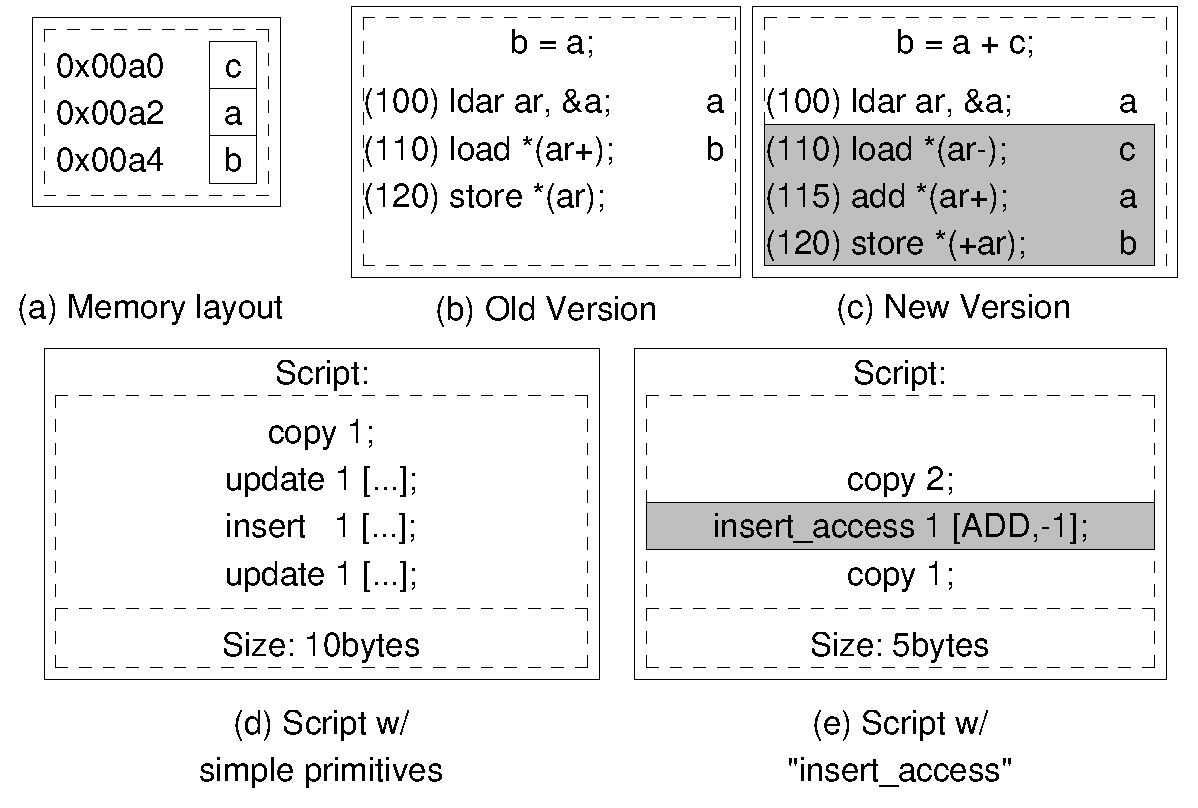
\includegraphics[width=4in]{./figures/insacc.eps}
\caption{An example showing the use of {\tt insert\_access} primitive:
(a) data allocation for both versions;
(b) the original code;
(c) the modified code;
(d) update script using simple primitives;
(e) update script using advanced primitives.
}
\label{insacc}
\end{center}
\end{figure}
	
When inserting a new memory access between two existing accesses, we may need two {\tt replace} primitives and one {\tt insert} primitive, as shown in Figure \ref{insacc}(d). Since the update primitives only modify the addressing modes, a compact way to express it is to include the memory address difference in the script and let the mobile devices generate the correct addressing modes for the related instructions. Thus, I introduce an {\tt advanced primitive} -- {\tt insert\_access}.

The {\tt insert\_access} primitive is similar to the {\tt insert} primitive, except that its data field is specified as follows:
\begin{eqnarray}
[\textit{operation},\delta_{\textit{diff}}]\nonumber
\end{eqnarray}
where $\delta_{\textit{diff}}$ represents the address difference between the locations accessed by the current instruction and the preceding instruction respectively. In the example (Figure \ref{insacc}(c)), the new access is {\em c }(located in memory slot 0), and the preceding memory access is {\em a} (located in memory slot 1), so $\delta_{\textit{diff}}$ is -1.
Since it is the add operation that accesses {\tt c} in the new instruction, the update primitive is  
\begin{eqnarray}
 \texttt{insert\_access} ~~~1 ~~ [\tt{ADD}, -1].\nonumber
\end{eqnarray}

Rewriting the update script of the example, using the {\tt insert\_access} primitive, the script size is reduced by 50\% (Figure \ref{insacc}(e)). 

The {\tt insert\_access} primitives allows the sensors to correct the
addressing modes before and after the newly inserted memory access.

Let us call the memory access instruction before the inserted instruction the {\tt 
predecessor} and the one that is executed after the inserted instruction the
{\tt successor}.
Based on these two instructions, the offset between them can be calculated.
The {\tt insert\_access} primitive encodes the offset between the inserted
memory access and the {\tt predecessor}, thus the offset between each two 
instructions among these three can be calculated.
Based on that information, the addressing modes can be determined.

\begin{figure}[htbp]
\centering
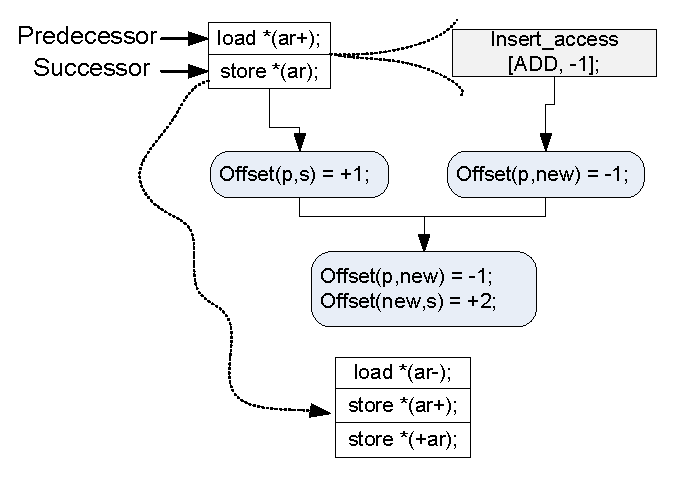
\includegraphics[width=3.5in]{./figures/insert_access.eps}
\caption{An example of the {\tt insert\_access} primitive interpretation procedure.}
\label{insertaccess}
\end{figure}

Figure~\ref{insertaccess} demonstrates the interpretation procedure of the
example given in Figure~\ref{insacc}. Knowing the offset between the {\tt predecessor}
and the inserted instruction is -1, and the offset between the inserted
instruction and the {\tt successor} is +2, the addressing mode of the 
{\tt predecessor} can be determined to be pre-incremental, that of the inserted
instruction can be determined to be post-incremental and that of the
{\tt successor} can be determined to be pre-incremental.

\subsection{Sensor-side primitive interpretation}

The received patch scripts will be stored in the program memory.
When the script download is complete, the sensors will run a simple script
interpreter to incrementally reconstruct the new binary image.
The reconstruction is based on the received the patch script and
the old binary image which is stored in the program flash on the
sensors.
The generated new binary image will be stored in the program flash as well.
When the primitive interpretation is complete, the sensors will load
the new binary image back to the program memory and restart
to execute the new version.
The old image will be kept in the program flash until the space is 
needed to store newer versions, so that when an execution error
happens, the sensors can roll back to the older version.
However, because sensors use cyclic redundancy check (CRC) to ensure the data integrity
while transmitting the patch messages, and the reconstruction
has been tested on the server side to make sure that it can generate
the correct binary image, there is a very small chance that the
new binary image is not functioning correctly.


The flash memory used to store both the old and new binary images
can be read in a random access fashion, so the pointer that is pointing
to the old binary can be moved arbitrarily to access the code segment
needed to build the new binary.
However, one limitation of the flash memory is that it has to be programmed 
at block levels, e.g. 256 bytes on for mica2 sensors~\cite{mica2-power}.
In order to change one byte, the sensor has to read the correspond block into
program memory, modify it and then write it back.
Thus, the constructed new binary needs to be buffered in the program memory
first until it reaches the size of a flash block, then the code block will be
written to the program flash. The size of the temporary code buffer 
should be the multiplier of the block size.


The interpretation algorithm is presented in Algorithm~\ref{decode}.
Each script primitive is scanned once, and is interpreted to construct
the new binary. 
Besides that, the interpreter maintains two instruction pointers, one points to the old
binary image and the other points to the last instruction that has been generated
in the new binary image. 

To interpret the  {\tt insert} and {\tt replace} primitives, it copies the instructions from the data
part of the primitive to the new binary.  To interpret the {\tt copy} primitive, it copies
the instructions from the old binary image instead.
The two pointers are updated as well. The pointer in the new binary is always
moved to the end of the image. The pointer in the old binary is shifted according
to the number of bytes that were copied, removed or updated, according to the
script.


\begin{algorithm}
\singlespace
\begin{algorithmic}[1]
\singlespace
\REQUIRE{ Pointer to the beginning of the patch script $P_S$, \\
	Pointer to the beginning of the old binary $P_O$,\\ 
	Pointer to the beginning of the new binary $P_N$.}
\FOR{(; $P_S \neq {\it script}.end$; $P_S$= next primitive)}	
	
\STATE {\bf switch}( primitive\_type($P_S$)

\STATE \hspace{5 mm} {\bf case} insert:
\STATE \hspace{10 mm} {\bf write\_code\_buffer}($P_N$, insert\_data($P_S$), insert\_bytes($P_S$))
%\STATE \hspace{10 mm} $P_N$ += insert\_bytes($P_S$);
\STATE \hspace{10 mm} {\bf break}

\STATE \hspace{5 mm} {\bf case} replace:
\STATE \hspace{10 mm} {\bf write\_code\_buffer}($P_N$, replace\_data($P_S$), replace\_bytes($P_S$))
%\STATE \hspace{10 mm} $P_N$ += replace\_bytes($P_S$)
\STATE \hspace{10 mm} $P_O$ += replace\_bytes($P_S$)
\STATE \hspace{10 mm} {\bf break}

\STATE \hspace{5 mm} {\bf case} copy:
\STATE \hspace{10 mm} {\bf write\_code\_buffer}($P_N$, $P_O$, copy\_bytes($P_S$))
%\STATE \hspace{10 mm} $P_N$ += copy\_bytes($P_S$);
\STATE \hspace{10 mm} $P_O$ += copy\_bytes($P_S$)
\STATE \hspace{10 mm} {\bf break}

\STATE \hspace{5 mm} {\bf case} remove:
\STATE \hspace{10 mm}  $P_O$ += remove\_bytes($P_S$)
\STATE \hspace{10 mm} {\bf break}

\STATE \hspace{5 mm} {\bf case} shift:
\STATE \hspace{10 mm} add $\left[ A1(P_S), A2(P_S), S(P_S)\right]$ to addr\_shift\_table
\STATE \hspace{10 mm} {\bf break}

\STATE \hspace{5 mm} {\bf case} clone:
\STATE \hspace{10 mm} {\bf if} ([start\_addr($P_S$), end\_addr($P_S$)] is not in clone\_buffer)
\STATE \hspace{15 mm} load code [start\_addr($P_S$), end\_addr($P_S$)] $\Rightarrow$  clone\_buffer;
\STATE \hspace{10 mm} {\bf endif}
\STATE \hspace{10 mm} replace\_register(buffer,register\_pairs($P_S$) )
\STATE \hspace{10 mm} {\bf write\_code\_buffer}($P_N$, buffer, clone\_bytes($P_S$))
\STATE \hspace{10 mm} {\bf break}

\STATE \hspace{5 mm} {\bf case} insert\_access:
\STATE \hspace{10mm} update the addressing mode of $P_N-1$ if necessary
\STATE \hspace{10mm} generate the addressing mode $addr\_mode$ for the inserted instruction
\STATE \hspace{10mm} instruction $i$ = form\_inst(opcode($P_S$),$addr\_mode$)
\STATE \hspace{10mm} {\bf write\_code\_buffer}($P_N, i$, length($i$))
\STATE \hspace{10mm} {\bf break}

\STATE \hspace{5mm} {\bf default}:
\STATE \hspace{10mm} error(``no such primitive'')
\STATE {\bf end switch}
\ENDFOR
\STATE copy new\_binary to program\_memory
\STATE restart the sensor
\end{algorithmic}
\caption{Primitive interpretation and code reconstruction.}
\label{decode}
\end{algorithm}

When encountering the {\tt shift} primitive, one entry that records the start address, end address
and shift offset is inserted to the shift table. To interpret the {\tt clone} primitive, the
master copy will be read from the program memory and register usage will be modified
to construct the cloned copy. The master copy needs to be read 0 to $K$ times, where
$K$ is the number of cloned copies that it has. In order to avoid reading the program
memory $K$ times, this master copy can be buffered in the program memory.
The {\tt insert\_access} primitive will decode the predecessor
and the successor to correct the addressing mode. Because the generated code is first
buffered in program memory, and there is usually one or two instructions inserted by
this primitive, both the predecessor and successor may still in the temporary code buffer.
Thus, this operation may not cause read or write to the new binary image.

When the whole code construction process is complete, the new binary image
will be copied to the program memory from the program flash. The sensor will
then restart to run the new code.




The algorithm shown in Algorithm~\ref{copycode} is called whenever a 
instruction is constructed and written to the temporary code buffer.
A simple decode operation is done first to filter out the branch instructions.
If the target address of the branch instruction falls in any range that needs address
shifting, this instruction will be updated to update the address.
When the temporary buffer is full, the code block will be copied to the
program flash.


\begin{algorithm}
\singlespace
\begin{algorithmic}[1]
\singlespace
\REQUIRE{ Destination address \& $P_N$, \\
	Source address $P_O$,\\
	Number of bytes to be copied $nbytes$.}
\STATE memcpy($P_N$,$P_O$,$nbytes$);
\FORALL{ instructions $i$ to be copied}
	\IF {inst\_type($i$) == branch/jump}
		\STATE $target$ = target\_addr($P_N$)
		\IF {there exists a shift entry $e\in$ shift\_table, where $target\in \left[ e.A1, e.A2\right]$}
			\STATE $target = target+e.S$
			\STATE change the target address of $P_N$ to $target$
		\ENDIF
	\ENDIF	
\ENDFOR
\STATE $P_N$ += $nbytes$
\IF {$P_N == {\it code\_buffer}.end$}
	\STATE write\_to\_flash(\it code\_buffer)
	\STATE $P_N = {{\it code\_buffer}}.begin$
\ENDIF
\end{algorithmic}
\caption{{\bf write\_code\_buffer} \/\/write the constructed code into code buffer}
\label{copycode}
\end{algorithm}

The memory space required for the interpreter include the temporary code buffer
and the shift table. As discussed before, the minimal size of the code buffer is the block
size of the program flash, which is 256bytes for Mica2 sensor.
Each entry of the shift table includes the start address, end address and the shift offset.
As the program memory size is 4Kbytes, the start address and end address can be
encoded using 3bytes. The shift offset can encoded using 1byte. Thus, the storage
required for each entry is 4bytes.


\section{Data based patching}



In the experiments, I observed that binary changes at several places may be caused by one memory layout change. For example, assuming variable {\tt a} appears in several places in the code and is relocated to a new memory location, we may generate a script with multiple update primitives each of which summarizes an instruction level change. Instead, if the script interpreter on mobile devices can decode DSP instructions, and identify all its uses, then it is possible to send one ``relocate {\tt a}'' primitive instead of individual instruction update. 

Let us call the binary instructions that are inserted, removed, or changed due to the offset assignment changes as {\tt Addressing Mode Change} (AMC) instructions. The motivation of developing {\tt data primitives} is to reduce the transmission of AMC instructions, and let the mobile devices construct them by themselves. Compared to the 
{\em insert\_access} primitive, data primitives are designed to update the code in more than one place.

\subsection{Data update primitives}
\begin{figure}[htbp]
\centering
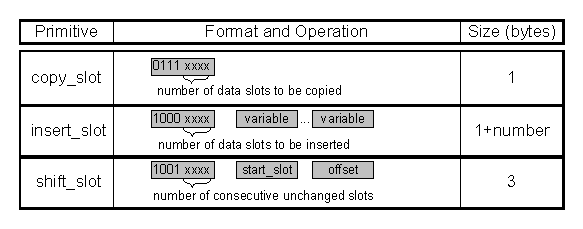
\includegraphics[scale=1.2]{./figures/fopcodedata.eps}
\caption{The patch script primitives -- data part.}
\label{fdatascript}
\end{figure}
In order to update the AMC instructions automatically, the offset assignment changes (rather than affected instructions) need to be transmitted. 
Figure \ref{fdatascript} lists the {\em data} update primitives that are used to specify the memory layout change. I only consider the allocation of scalar variables here. Each memory location contains one variable or multiple coalesced variables (\cite{related:ottoni,related:zhuang}). 

\subsubsection{copy\_slot.}  This primitive copies multiple memory slots from the old offset assignment to the new assignment. There are two pointers pointing to the new and old assignments respectively. They are updated to the next slot with this primitive.

\subsubsection{insert\_var.} This primitive adds a list of variables to the current memory slot in the old assignment. The related slot with the added variables is then copied to the new assignment. The insertion can be caused by adding a new variable, or by moving an existing variable from another location. The latter implicitly has the variable removed from the old location, which is omitted to keep the script compact. 

\subsubsection{shift\_slot.} This primitive represents the case that multiple slots may be grouped and shifted from the old assignment to the new assignment. The {\tt shift\_slot} primitive specifies the number of slots that need to be shifted, the starting point of the shift, and the shift offset.


\subsection{Sensor-side primitive interpretation}

After receiving the update script, each sensor interprets the {\em data update primitives} to generate the new memory layout, and then interprets the {\em code update primitives} to construct basic blocks by inserting, removing, or updating certain instructions on top of the old binary version. The interpreter fixes the addressing mode of each instruction in a basic block according to the new memory layout, and then writes the completed block into the flash.


\begin{figure*}[htbp]
\begin{center}
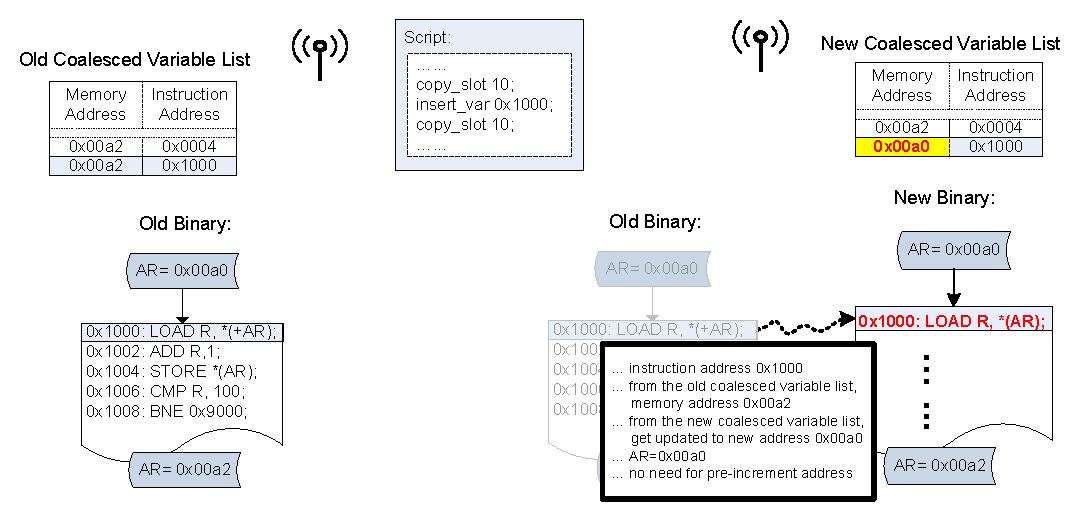
\includegraphics[width=6in]{./figures/correct.eps}
\caption{The code construction procedure of the data primitives (The left shows the server side, and the right shows the mobile device side updates).}
\label{codecorrection}
\end{center}
\end{figure*}

However, it may require additional information to fix the addressing modes on the mobile device side. As shown in Figure \ref{codecorrection}, CSOA coalesces multiple variables --- both {\tt a} and {\tt e}, in one memory location {\tt 0x00a2}, a code update may re-allocate {\tt e} to {\tt 0x00a0} while keeping {\tt a} in the same memory slot. This complicates the code update as some accesses to {\tt 0x00a0} should be updated while others should not.

Figure \ref{codecorrection} illustrates my solution to this problem. 
I use an implicit pointer to track the current memory slot when copying from the old layout to the new layout.  ``{\tt insert\_var} {\tt 0x1000}'' inserts~{\tt e} into the current slot, i.e. {\tt 0x00a0}. Here variable {\tt e} is represented using its instruction address {\tt 0x1000}. A record can be found in the coalesced variable list indicating this mapping, and will be updated to reflect to the re-allocation.

To update the addressing mode in the new code, a query is sent to the coalesced variable list, from which we know this instruction accesses {\tt 0x00a0} instead of {\tt 0x00a2}. Since AR contains {\tt 0x00a0} when entering the basic block, there is no need for pre-increment. Similar decisions are made for other instructions in the basic block and ensure the exiting AR contains {\tt 0x00a2}.

From this discussion, the interpreter needs the following information to fix the addressing modes:
\begin{itemize}
	\item A coalesced variable list to distinguish each of coalesced variables; and
	\item The AR values when entering and exiting each basic block.
\end{itemize}

\subsubsection{Auxiliary data structures}
To correctly update the code with a memory layout change, e.g. {\tt a} is assigned to a different memory location, we need to locate all of {\tt a}'s uses and ensure the AR contains the correct address when accessing {\tt a}. Conceptually, this can be done by a relocation table. Unfortunately a traditional relocation table identifies all the places that the binary code accesses the memory. Since DSP code relies heavily on offset assignment and accesses the memory frequently, adopting a traditional relocation table would generate a table linear to the size of the binary code. Instead, I introduce the following two lightweight auxiliary data structures to enable relocatable DSP code.

{\bf Coalesced variable list.}
The coalesced variable list is designed to differentiate the coalesced variables in one memory location. If a memory location contains only one variable, then the scheme does not allocate any entry in the list. If multiple variables are coalesced and stored in the same memory location, the scheme allocates the entries as follows. 

\begin{figure}[htdp]
\begin{small}
\begin{center}
\begin{tabular}{p{1in} p{1in} }  \hline
Memory  & Instruction  \\
Address & Address \\ \hline\hline
0x00a2 & 0x0004  \\
0x00a2 & 0x1000  \\ \hline
\end{tabular}
\end{center}
\caption{Coalesced variable list.}
\label{memvar}
\end{small}
\end{figure}

Since the coalesced variables have their accesses spread in the code, I group consecutive definitions/uses that access the same variable and allocate one entry to each group. This is done based on the code text without considering the control flow, or the variable live range etc. For example, if the live ranges of two coalesced variables overlap due to linear layout of control structures such as branches, then we allocate one entry for each segment. As shown in Figure~\ref{memvar}, each entry contains two fields: the memory slot address, and the starting instruction address of each code text segment. 

For example, variable {\tt a} and {\tt e} share the same memory location {\tt 0x00a2}. The live ranges of {\tt a} and {\tt e} are {\tt [0x0000,0x0004]} and {\tt [0x0010,0x1000]} respectively. Figure \ref{memvar} illustrates its coalesced variable list. Given a memory access to {\tt 0x00a2}, we can easily differentiate whether it is accessing {\tt a} or {\tt e}.

The original coalesced variable list is preloaded on the mobile devices before deployment. The updates to the coalesced variable list is transmitted with the code update script. The coalesced variable list update primitives will be discussed later.

{\bf AR in/out value list.} 
As discussed before, we need the AR in and out values for each basic block in order to generate the correct addressing modes on the mobile device side. I choose to construct the list rather than building the control flow graph on demand to reduce the memory and complexity overheads. This table contains the starting, ending addresses, the address register's entering, exiting values and the successive basic block(s) of each basic block, as shown in Figure \ref{bbtable}.

\begin{figure}[htdp]

\begin{center}
\begin{small}
\begin{tabular}{p{0.5in}p{1in}p{1in}p{1in}p{1in}p{1in}}
\hline
Index & Starting  & Ending  & AR In & AR Out & Successive \\
&Address&Address & & &Basic Blocks\\
\hline\hline
10 & 0x1000 & 0x1008 & 0x00a0 & 0x00a2 & 20\\ \hline
\end{tabular}
\end{small}
\end{center}
%\vspace{-0.1in}
\caption{The AR in/out value list.}
\label{bbtable}
%\vspace{-0.1in}
\end{figure}%

The original list is preloaded on the mobile devices before deployment. The interpreter automatically generates the new list while generating the new binary code. 

The AR out value of a basic block may affect the addressing mode of its successive basic blocks. The situation becomes more complicated if there are multiple predecessors (or successors). Synchronization needs to be done among these predecessors (or successors), which may cascadingly affect other instructions in those basic blocks. To simplify the code update on mobile device side, the server explicitly sends out the AMC instructions that follow an inserted/updated/removed instruction, and those that are the last instruction of a basic block.

{\bf Complexity analysis.}
The following pseudo code Algorithm~\ref{datadecode} presents the algorithm that is used to correct the addressing modes based on the data change primitives. The extra interpretation overhead is to look up the address register value for the first instruction of each basic block, keep track of this value while constructing the instructions in the basic block, and generate the correct addressing mode for each memory access instruction. However, addressing mode correction is only necessary 
when the data layout is changed for the corresponding code segment. For example, if the highlighted variable list change is the only memory layout change in the example shown in Figure~\ref{codecorrection}, the instructions before 0x1000 do not need to be decoded, because the memory layout change do not affect those instructions.



\begin{algorithm}
\singlespace
\begin{algorithmic}[1]
\singlespace
\REQUIRE{Instruction {\bf $i$} which will be copied from old binary to the new binary,\\
address of this instruction in the old binary {\bf $addr1$},\\
address of this instruction in the new binary {\bf $addr2$}}
\ENSURE{Instruction $i'$ which has the same opcode as $i$ and with the addressing mode corrected}
	\IF{inst\_type($i$) is memory access instruction}
		\STATE\COMMENT {find out the value stored in address register (AR)}
		\IF{$i$ is the first instruction of basic block $B1$ in old binary}
			\STATE $old\_ar\_value$ = query\_old\_AR\_tab($B1.AR\_in$)
		\ENDIF	
		\IF{$i$ is the first instruction of basic block $B2$ in new binary}
			\STATE $new\_ar\_value$ = query\_new\_AR\_tab($B2.AR\_in$)
		\ENDIF
	\STATE	
	\STATE\COMMENT{find out the memory address that this instruction tries to access}
	\STATE $old\_mem\_addr$ = gen\_addr\_mode($old\_ar\_value$, addr\_mode($i$))
	
	\STATE\COMMENT{find out the variable that this instruction tries to access}
	\STATE $var\_name$ = query\_old\_var\_tab($old\_mem\_addr$, $addr1$)
	
	\STATE\COMMENT{find out the new memory location of this variable}
	\STATE $new\_mem\_addr$ = query\_new\_var\_tab($var\_name$, $addr2$)
	\STATE
	\STATE\COMMENT{generate the new addressing mode and construct the instruction}
	\STATE $addr\_mode$ = form\_addr\_mode($new\_mem\_addr$,$new\_ar\_value$)
	\STATE instruction $i'$ = form\_inst(opcode($i$),$addr\_mode$)
	\STATE return $ i'$
	\ENDIF	
\end{algorithmic}
\caption{{\bf addr\_mode\_correction} /*Correct the addressing mode of an instruction*/}
\label{datadecode}
\end{algorithm}



Each entry of the ``coalesced variable list'' is 4 bytes, and each entry of the ``AR in/out value list'' is 9 bytes,
so they can both fit in the program memory for fast access.

\chapter{Distribution protocol}

As introduced in Chapter~\ref{chap:intro}, there are two circumstances in software update,  software upgrade and 
software switch. The software upgrade happens when the application that is already running in the WSN needs to be 
changed for bug fix or adding new features. So in this case, there is one source node -- the sink, and multiple 
destination nodes in the network. However, The software switch happens in MA-WSNs, where multiple applications are 
already deployed in the network. Because some neighboring nodes may already have the wanted binary code in memory, the 
code distribution problem here is how to route the code image from sensors to sensors. In this case, there are multiple 
source nodes in the network, which is different from the software upgrade case. Because of this difference, I propose 
to use two different code distribution protocols for the two different cases.


\section{Broadcast based code distribution protocol (Deluge)}
While doing software upgrade, the upgrade patches are generated on the sink node using the proposed update-conscious 
compiler techniques to improve the code similarity with the older version of such application. Then the patch is 
generated in the script format as mentioned above.After the patches are generated on the sink node, the network 
protocol Deluge~\cite{deluge} is used to disseminate the scripts to the network. 

The protocol works as follows. 
First, the whole update script is divided into fixed size pages.
At the beginning, the states of nodes are set to {\it Maintain} state. 
Each sensor node keeps broadcasting the advertisement messages ({\it ADV}) periodically,
which contains the information of the application code that it has. 
When a sensor node {\it S} receives an advertisement, which indicates that the neighbor 
{\it N} has a newer version of the application in its memory or has finished downloading more pages, node S will send 
out a request message ({\it REQ})
to {\it N} to request for a page, and change its own state from {\it Maintain} to {\it Request}.
The state will be changed back when it receives all the packets in the requested page.
Node {\it N} will change state to {\it Transmit} when it receives the request message from
{\it S}. Then it will start sending all the packets of the requested page to node {\it S}.
After the code transmission is finished, the state will be changed back to {\it Maintain} state.
Figure~\ref{fdeluge} shows the advertise-request-data handshaking protocol used Deluge~\cite{deluge}.

\begin{figure}[htbp]
\centering
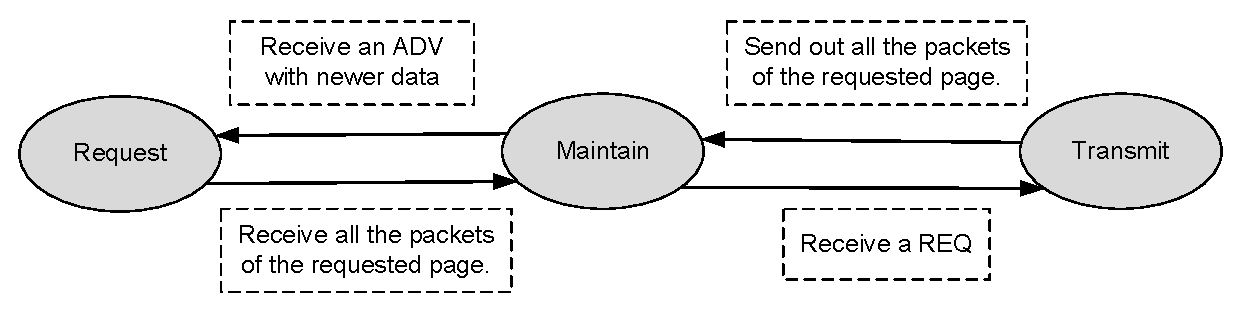
\includegraphics[width=4.2in]{figures/deluge.eps}
\caption{Advertise-request-data handshaking protocol in Deluge.}
\label{fdeluge}
\end{figure}

These packets may be
encrypted and/or authenticated for security protection~\cite{sluice,secDiss1}. The
packets may also be grouped so that when remote sensors receive groups
out of order, they are still able to perform updates independent of
the receiving order.


\section{Multicast-based code redistribution protocol (MCP)}
	
\subsection{The software switch problem in MA-WSNs}
	
While doing software switch, the problem is a little bit different. The following example shown in Figure~\ref{fnet} 
illustrates the protocol design challenges here. 
Three applications are distributed across different nodes in a network. The code distribution problem arises when there 
is a need to reprogram some nodes to run application {\it A}.

\begin{figure}[htbp]
\begin{center}
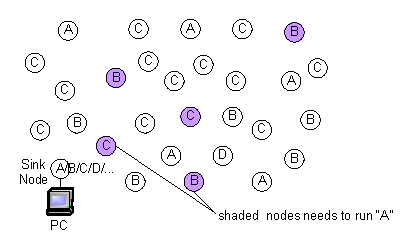
\includegraphics[width=3in]{figures/fnet.eps}
\caption{An example of software switch in a multi-application WSN (MA-WSN).}
\label{fnet}
\end{center}
\end{figure}

There are two existing approaches. A naive solution is to directly apply Deluge and disseminate application {\it A} 
from the sink to all sensors. After dissemination, the nodes that do not need {\it A} discard the code from their 
storage. The solution is clearly not a good choice due to unnecessary packets transmissions to the nodes that don't 
need it. The other solution is to let requesting nodes initiate code dissemination and fetch {\it A} from nearby 
sensors. Melete~\cite{melete} is such a protocol --- the nodes that need to run {\it A} broadcast their requests within 
a controlled range and discover the source nodes that have {\it A}. Sources then send back the requested data packets. 
However, as a stateless protocol, Melete does not record the source nodes and has to discover them repeatedly. When 
transmitting applications with multiple pages, multiple sources within the range may respond and thus create 
significant signal collision. 


\subsection{A multicast-based code redistribution protocol (MCP)}


I propose a multicast-based code redistribution protocol,  MCP, to solve the ``n to n'' code distribution problem in 
software switch. MCP employs a gossip-based source node discovery strategy. Each sensor summarizes the application 
information from overheard advertisement messages, and stores this information in a local application information table 
(AIT). Future dissemination requests are forwarded to nearby source nodes rather than flooding the network.
Different from the Deluge~\cite{deluge} scheme discussed above, the data messages are only multicast to the requesters, 
which avoids the unnecessary packet transmission in the network. With the guide of AIT, the request messages can be 
directly sent to the source nodes, which avoids the request message flooding in the network.  

An overview of this protocol is as follows.

\begin{itemize}
\item 
Sensors in MCP periodically broadcast {\it ADV} messages to advertise their knowledge about running applications in the 
network, which is similar to Deluge. Each sensor summarizes its overheard {\it ADV} messages in an {\em application 
information table (AIT)}. 

\item
To reprogram a subset of sensors, the sink floods a dissemination command that guides which sensors should switch to 
run application {\it A}. For example, a command ``[B$\rightarrow$A, p=0.25]'' indicates that the sensors whose active 
application is ``B'' should switch to ``A'' with a 25\% probability. That is 25\% of the nodes that are currently 
running application ``B'' will switch to ``A''.

\item
After receiving the command from the sink, each sensor identifies its dissemination role as one of the followings.  \\
(i)  a {\em source} if the sensor has the binary of application {\it A}; \\
(ii) a {\em requester} if the sensor does not have the binary of {\it A} but needs to switch to run {\it A}; or  \\
(iii) a {\em forwarder} if the sensor is neither a {\em source} nor a {\em requester}.

\item
A {\em requester} periodically sends out requests (i.e., {\it REQ} messages) to its closest source, until it acquires 
all the pages of application {\it A}. Instead of broadcast, the {\it REQ} messages are sent to the source via 
multicast. A requester resends the {\it REQ} message until it timeouts. It tries to request data from each source node 
several times before marking the node as a {\em temporary non-available} source.

\item 
A source node responds with the data (i.e., {\it Data} messages) that contain code fragments while a forwarder forwards 
both request and data packets. 
\end{itemize}

Similar to Melete and Deluge, MCP has three types of messages: an {\it ADV} message that advertises interesting 
applications; a {\it REQ} message that asks for packets of a particular page; and a {\it Data} message that contains 
one data packet (i.e, a piece of code segment).

\subsection{ADV message and application information table (AIT)}
In MCP, each sensor periodically broadcasts ADV messages, and summarizes the information of overheard ADV messages into 
a small application information table (AIT). Fig. \ref{fait} illustrates the algorithm.

Each {\it ADV} message contains the information of one application: (i) an application ID and version number; (ii) the 
number of pages of the application; (iii) the information of two closest source sensors --- the source ID and number of 
hops to the source (S, H); (iv) the CRC checksum. 
If a sensor has multiple known applications, it advertises them in a round-robin fashion. Note that a sensor may not 
have the code images of all its known applications. 

\begin{figure}[htbp]
\begin{center}
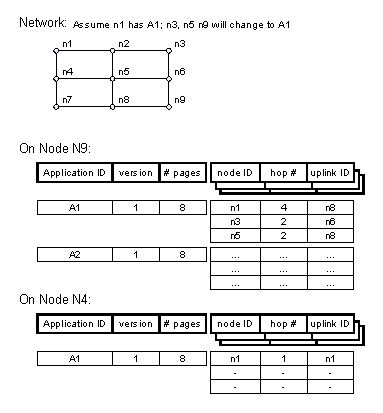
\includegraphics[width=4in]{figures/ftable.eps}
\caption{An example of the application information table (AIT).}
\label{fait}
\end{center}
\end{figure}




The AIT summarizes the overheard ADV messages. In addition to the application summary, AIT stores up to three closest 
source nodes for each known application, and the uplink sensor ID for each source, i.e., from which the source 
information was received.
The size of each application entry in the AIT is 12 bytes. Assume that the number of the applications running in the 
network is 10,
the AIT size will be only 120 bytes, which makes it fit perfectly in the program memory.

When an incoming ADV message contains new information, the corresponding entry in the AIT is updated. Assume a sensor 
S1 receives an ADV message from S2, and the message identifies two nearby sources (S3, H3) and (S4, H4) where H3 and H4 
indicate the number of hops from S2 to sources S3 and S4. If S1 already records the information of three sources (S5, 
H5, U5), (S6, H6, U6), and (S7, H7, U7), then it updates the AIT table according to the following rules. 

\begin{itemize}
\item
If one entry in AIT table records the previous message from the same uplink S2 and it refers to the same source, e.g. 
S5=S3 and U5=S2, then the information in the ADV message represents the up-to-date source information and replaces the 
old entry.

\item
If one entry in the AIT records a longer path to an advertised source, e.g. S5=S3, U5$\ne$S2, and H5$>$(H3+1), then the 
hop count and uplink node from the ADV message replace those in the AIT.

\item
If the advertised source cannot be found in the AIT, and there is an invalid entry in the table, then the new source is 
inserted into the table.

\item
If the ADV message advertises a closer source than one of those in the AIT table, then the closer source replaces the 
farthest source in the AIT. 

\end{itemize}

Each sensor advertises the application in the AIT in a round-robin fashion, and prioritizes the applications whose 
entries have been recently updated: (i)~the applications whose sources were recently updated are advertised before 
those that were not; (ii) in one round, the applications whose sources were recently updated are advertised three times 
while others are advertised once. In addition to normal ADV advertisement, an application is advertised if the sensor 
receives a broadcast request for that application, as we elaborate next.

\subsection{Request multicasting}
In MCP, a requester continues to send out request messages until it receives all pages of the target application. Given 
the target application, the requester searches the AIT for a closeby live source and constructs a REQ message as follows
\begin{center}
REQ = [S, H, pgNum, bv] \\
\end{center}
where S indicates the selected source node, H indicates the maximum number of hops that the message may travel, pgNum 
and bv indicate the current working page and the requested packets in the page. If the AIT records more than one source 
node, then the requester selects the closest live source and sets H to h+$\delta$ where h is the number of hops to S 
(recorded in the AIT), and $\delta$ is the hop count slack allowed in the dissemination. 
Fig. \ref{fgrad} illustrates the involved nodes when h=2 and $\delta$=1. These nodes routed through a gradient-based 
region~\cite{groute} to the source. 

\begin{figure}[htbp]
\begin{center}
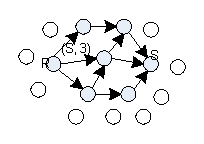
\includegraphics[width=1.5in]{figures/fgrad.eps}
\caption[Gradient-based request routing.]{Gradient-based request routing. R and S are requester and source nodes 
respectively; h=2; $\delta$=1.}
\label{fgrad}
\end{center}
\end{figure}

A requester continues sending the REQ messages when it can not finish the page before timeout. After several tries, it 
marks the source that it tried
to reach as an {\em unreachable} source. The number of tries varies based on the distance to the source. 

If the AIT does not record any nearby source, then the requester sets~S to be {\em null}, indicating the REQ message is 
sent to all neighbors. After receiving a broadcast request, an idle forwarder forwards the request unless the message 
has travelled the maximum number of hops; an idle source node always responds with requested packets.

%If the sensor records a local source in its AIT, however the corresponding uplink of the AIT entry is not the node 
from which the request was %received, the sensor advertises the source information. 

Since each requester sends out REQ messages independently, different requesters may work on different pages. MCP allows 
node preemption. If a REQ message asking for page $x$ reaches a working node who is currently working on page $y$, and 
$x+1 < y$, then the node quits the current state and switches to serve the request. If the node is a forwarder, then it 
forwards the request; if the node is a requester or a source, then it must have the requested page and thus will 
respond with the requested packets. The node enters the idle state after serving the request.

\subsection{Caching}
During code dissemination, some requesters or forwarders, while working on the current page, may overhear packets from 
pages with larger indices. As code pages are requested strictly in increasing order, a requester will work on 
large-number-indexed pages, and a forwarder has a high possibility to receive requests for these pages. 

To improve transmission efficiency, sensors in MCP buffer such packets in their data memory. The space that can be 
dedicated to caching on a wireless sensor is usually very limited. While it is possible to exploit external flash for 
caching, accessing external flash is slow and writing it has to be performed in 256-byte blocks, which complicates the 
design and wastes the energy. 

Caching on a requester is straightforward as the sensor always caches the next several pages in addition to the current 
working page. However, it is slightly more complicated on a forwarder node as it gets requests from different 
requesters that work on different pages and may suffer from thrashing if it takes turns to serves these requests. In 
MCP, a forwarder gives priority to pages with smaller indices. We set a timer for the cached page and clear the page 
after serving a request or timeout.


\section{Simultaneous code dissemination}
As shown in~\cite{melete}, different applications in a MA-WSN
usually share some code segments. For example, two applications
may be designed for sensing and processing two different
events like wildfire and animal mitigation. While the
data processing components are different, the routing code
could be similar. If one application has already been installed
on some sensors, then at the time when a remote sensor
wants to load the other application, it is energy efficient
to fetch the common code from these peer sensors instead of
the sink. 

Fetching code from peer sensors exhibits two advantages:
(i) remote requesting sensors (i.e. the sensors that
need to switch their running application to the new one) can
start early and fetch the code in parallel without waiting for
the progressive code dissemination from the sink. (ii) since
only a subset of sensors get involved in dissemination, the
message overhead can be greatly reduced. Without losing
generality, we assume $A$ and $B$ share $S_{ab}$ common packets
while $A$ and $C$ do not share any packet. When a sensor
needs to switch to run application $A$, it fetches shared code
from nodes that have $B$ and the rest of the code from the
sink.

\begin{figure}[htbp]
\begin{center}
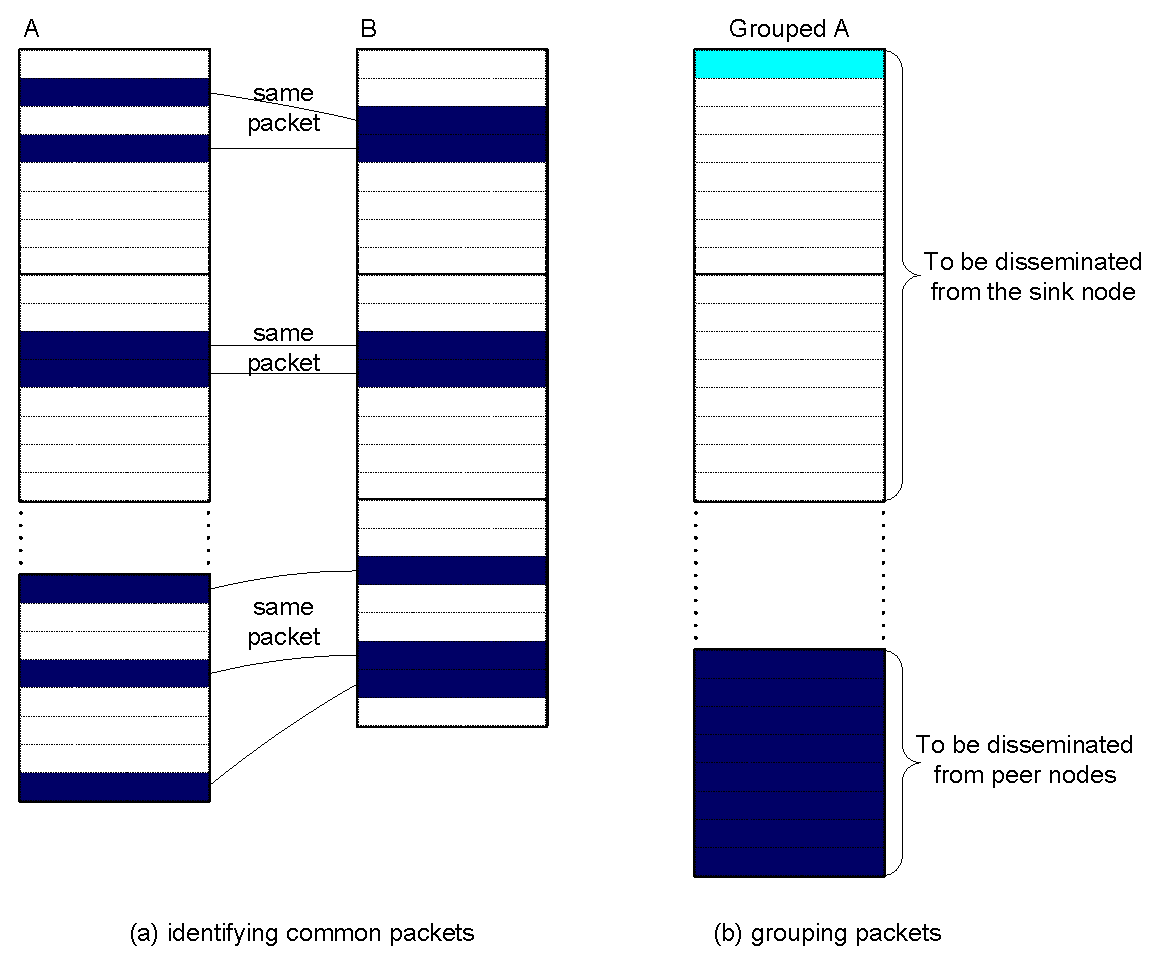
\includegraphics[width=4.5in]{figures/common.eps}
\caption{Simultaneous code dissemination.}
\vspace{-0.3in}
\label{common}
\end{center}
\end{figure}

The basic dissemination unit in MA-WSN is a packet
that contains 23 bytes payload, similar as that in the default
multi-hop dissemination protocol Deluge~\cite{deluge} in TinyOS. To
enable code dissemination of two types of packets, the code
segments needs to be reorganized, as shown in Fig~\ref{common}. Given
the above application $A$ to be disseminated, we first divide
it into a sequence of code packets, and mark all packets
that are shared with $B$. We compare at the packet level in
this paper while techniques have been proposed to compare
two applications and generate difference at different levels
~\cite{melete,ucc} After marking the code, we group packets based
on if they are marked or not, and add two bit vectors (one
vector per application and one bit per packet) to guide the
code reorganization. The bit vector for application $A$ (or
$B$) indicates the locations of marked packets in application
$A$(or $B$). For example, a bit vector 
\chapter{Experiment results}


\section{Benchmarks}
Because the software update management is a new problem to study
in the wireless embedded system community, there is no existing
update benchmarks available to evaluate the performance gain
of my proposed framework.
Therefore, I built a sensor software update benchmark suite
which covers the software update cases for both general purpose
applications and DSP applications that run on the wireless
embedded devices.

The base benchmarks are from the general purpose
sensing applications included in TinyOS~\cite{tinyos}--
an open-source operating system designed for wireless embedded
sensor networks, CryptoLib -- the encryption library, and the DSP applications included in 
DSPstone~\cite{dspstone} benchmark suite. 
Upon the base benchmark, I created the pairing update benchmark
using three different techniques and categorized them based on the update levels.

\subsection{Update levels}
There are three update levels according to their
impact on code structures: (a) small changes, which are made to local
basic blocks; (b) medium changes, which include changes in a large
function or across several functions, but still preserve the overall
structure of the original code; (c) large changes, which significantly
change the code structure. Frequent updates such as code fixes and
sensor reconfigurations are mainly small or medium changes, while
replacing the application with a new one introduces medium to large
changes. 

\subsection{Real update benchmarks}
One application may have multiple versions that exist in the
base benchmarks to add new features of fix bugs that exist 
in the old version.
For example, TinyOS-1.x has over 15 versions, and in each release
the enclosed applications may be updated.
Updates made to the applications vary from adding one statement
to completely reconstructing the code.
As the proposed software update management framework targets
at small or medium level code updates, I selected the proper sized real code
update cases that exist in the base benchmarks as the real update
benchmarks.
These real update benchmarks will show the real update patterns
for the applications running on wireless embedded devices and
become the base of generating the other two update benchmarks.

\subsubsection{Real general purpose application update benchmark}
Figure~\ref{fdeluge.src} shows one real update case of the general purpose
software.
The function unit Deluge~\cite{deluge}, a reliable code dissemination protocol
enclosed in TinyOS is studied.I studied updates of Deluge from TinyOS version 1.52 
to version 1.58. The update details are shown in the figure.

\begin{figure}[htbp]
\begin{center}
\begin{small}
\begin{tabular}{||p{0.5in}|p{1in}|p{0.6in}|p{3.5in}||} \hline

Case\# & Versions & Update Level & Update details \\ \hline \hline

R-G-1 &  ${1.52 \Rightarrow 1.53}$ & Small & Add one statement to reset one variable. \\ \hline
R-G-2 &  ${1.53 \Rightarrow 1.54}$ & Large & Add one variable, and related statements to
	update this variable when necessary. One statement is updated to use this variable instead. \\ \hline
R-G-3 &  ${1.54 \Rightarrow 1.55}$ & Medium & Modify the condition of two ``if'' statements. \\ \hline
R-G-4 &  ${1.55 \Rightarrow 1.56}$ & Large & Move one function. Add one ``if'' statement to reset 
	one variable when it's invalid, and all the other four related variables. \\ \hline
R-G-5 &  ${1.56 \Rightarrow 1.57}$ & Medium & Move two ``memcpy'' statements to be next to the relative ``if'' statements. \\ \hline
R-G-6 &  ${1.57 \Rightarrow 1.58}$ & Large & Modify the condition of two ``if'' statements. Add two ``for'' loops. Remove two statements. \\ \hline

\end{tabular}
\end{small}
\end{center}
\caption{Real general purpose application update benchmark. (Deluge in TinyOS 1.52-1.58.)}
\label{fdeluge.src}
\end{figure}

\subsubsection{Real DSP application update benchmark}
For the DSP applications, I selected the matrix multiplication function {\it matrix.c} and one function in the ADPCM standard implement {\it speed\_control} as the real DSP update benchmarks. More information can be found in Figure~\ref{dsp-bench}. 

\begin{figure}[htdp]
\begin{small}

\begin{center}
\begin{tabular}{||p{0.5in}|p{1.5in}|p{0.6in}|p{3.5in}||}
\hline
Case\#  &  Function & Update & Description \\
 & \& Versions &Level&\\
\hline\hline
R-D-1 &  matrix1.c$\Rightarrow$matrix2.c& medium & Move two iterations out of the loop.\\
\hline
R-D-2 &  speed\_control 1 $\Rightarrow$2 & medium &Seven temporary variables are introduced to hold the value of the comparison results.\\
\hline
R-D-3 & speed\_control 2 $\Rightarrow$3 &large &  Multiple global variables are combined into a structure. The reference to the variables are changed due to this change.\\
\hline
\end{tabular}
\end{center}
\caption{Real DSP application update benchmark. }
\label{dsp-bench}
\end{small}
\end{figure}%


\subsection{Manually generated update benchmarks}

\begin{figure}[htbp]
\centering
\begin{small}
\begin{tabular}{||p{1in}|p{0.5in}|p{4in}||} 
\hline
Base  & Source & Details \\ 
benchmark & & \\\hline  \hline

Blink & TinyOS & It starts a 1Hz timer and toggles the red
LED every time it fires. \\ \hline

CntToLeds & TinyOS & It maintains a counter on a 4Hz timer and
displays the lowest three bits of the counter value. The red LED is
the least significant of the bits, while the yellow is the most
significant. \\ \hline

CntToRfm & TinyOS & It maintains a counter on a 4Hz timer and sends
out the value of the counter in an IntMsg AM packet on each
increment. \\ \hline

CntToLeds AndRfm & TinyOS & It maintains a counter on a 4Hz timer; it
combines the tasks performed by CntToRfm and CntToLeds. \\ \hline

AES & Crypto Lib & It encrypts a given 128 bit input buffer using AES
algorithm. I select the encryption code in the experiment.\\ \hline \hline

Deluge & TinyOS & The mulithop code dissemination protocol in TinyOS. I tracked its continuous updates in different TinyOS versions as a real life case study. \\ \hline
\end{tabular}
\end{small}
\caption{Base benchmarks for general purpose applications.}
\label{fbench}
\end{figure}

Software updates are manually inserted to the base benchmarks to create the
manually generated update benchmarks.
The manual inserted code includes insertion/deletion variables, 
insertion/deletion instructions, changing 
existing instructions, and changing the control flow. 



\subsubsection{Manually generated general purpose application update benchmark}


The TinyOS application shown in Figure~\ref{fbench} are selected as the base benchmarks
to create the manaually generated general purpose software update benchmark.


Figure \ref{fbench.chg1} summarizes the synthetic updates made to these
benchmarks. The updates vary from small, through medium, to large changes.

\begin{figure}[htbp]
\centering
\begin{small}
\begin{tabular}{||p{0.6in}|p{1in}|p{0.5in}|p{3.5in}||} \hline
Case \# & Function & Update Level & Update details \\ \hline \hline

M-G-1 & CntToLeds &Small & Change the color of blink. \\ \hline

M-G-2 & Blink &Small & Insert one local variable and one use in
run\_next\_task. \\ \hline

M-G-3 & AES& Small & Insert one local variable and use it within the
loop in aes\_encrypt. \\ \hline

M-G-4 & AES & Small & Change one instruction in aes\_encrypt. \\ \hline

M-G-5 & AES & Small & Insert a local variable in aes\_encrypt and use it
twice --- within and outside the loop. \\ \hline

M-G-6 & Blink &Small &Add a new parameter in TOSH\_run\_task. \\ \hline

M-G-7 & CntToLeds & Medium & Insert three variables and their uses; \\
\hline

M-G-8 & CntToRfm & Medium & Insert a global variable and use in three
different functions. \\ \hline

M-G-9 & CntToRfm & Medium & Insert a local variable and use it several
times in TOSH\_run\_next\_task function. \\ \hline

M-G-10 & Blink&Medium & Insert a global variable and use it in a new
if/then branch in TOSH\_run\_next\_task function. \\ \hline

M-G-11 & Blink & Medium & Add an else branch for an if statement in Timer\_HandleFire. \\ \hline

M-G-12 & CntToRfms $\Rightarrow$ CntToLedsRfm &Large & Change the application from CntToRfms to CntToLedsRfm \\ \hline 

M-G-13* &CntToLeds$\Rightarrow$ CntToRfms &Large & Change the application from CntToLeds to CntToRfms. \\ \hline 

M-G-14 & AES & Medium & Add two and remove one local variables in function invShiftRows().
\\ \hline
M-G-15 & AES & Medium & Add one and remove two local variables in function invShiftRows().
\\ \hline

M-G-16 & AES & Medium & Add one local variable in function invShiftRows() and add a four element array in function invMixSubColumns().\\ \hline
M-G-17 & AES & Medium & Remove one local variable in function invShiftRows() and remove a four element array in function invMixSubColumns().\\ \hline


M-G-18 & AES & Large & Remove one and add two local variables in function invShiftRows(). Remove two and add four local variables in function invMixSubColumns().\\ \hline
M-G-19 & AES & Large & Add one and remove two local variables in function invShiftRows(). Add two and remove four local variables in function invMixSubColumns().\\ \hline

\multicolumn{4}{l}{*: The experimental results of this case are shown in the text instead of the graphs to make}\\
\multicolumn{4}{l}{the graphs more proportionally precise.}\\

\end{tabular}
\end{small}
\caption{Manually generated general purpose application update benchmark.}
\label{fbench.chg1}
\end{figure}


\subsubsection{Manually DSP application update benchmark}
For the DSP applications, I inserted/deleted code to create/remove the variable interferences to the DSP base benchmarks, such as the matrix multiplication function {\it matrix.c} and one function in the ADPCM standard implement {\it speed\_control} as the real DSP update benchmarks. 
The detailed benchmarks are listed in Figure~\ref{dsp-manual}. 

\begin{figure}[htdp]
\begin{small}

\begin{center}
\begin{tabular}{||p{0.5in}|p{0.6in}|p{1.2in}|p{3.5in}||}
\hline
Test &   Function & Update &Description \\
Case & & Level&\\
\hline\hline
M-D-1  & verify.c&small& Update \textbf{one basic block}  to create
the interference between two variables that are \textbf{not coalesced} 
in the original version.\\
\hline
M-D-2  & verify.c& medium & Update \textbf{one basic block} to create
the interference between three variables that are \textbf{coalesced}
in the original version. \\
\hline
M-D-3  & verify.c& medium & Expand the live ranges of three variables to
\textbf{cross basic blocks}. \\
\hline
M-D-4   & matrix1.c& medium & Shrink the live range of the one variable and
Expand the live range of another variable within on basic block.  \textbf{ Over
ten interferences} are updated.\\
\hline
M-D-5 & matrix1.c& medium  & Shrink the live ranges of the two variables and
Expand the live ranges of another two variables within on basic block.
 \textbf{Over ten interferences} are updated.\\
\hline
\end{tabular}
\end{center}
\caption{Manually DSP application update benchmark.}
\label{dsp-manual}
\end{small}
\vspace{-0.1in}
\end{figure}%

\subsection{Automatically generated update benchmarks}
In order to study more general cases and to evaluate the compiler performance,
I also wrote a tool to generate the update benchmarks automatically.

\subsubsection{Automatically generated general purpose application update benchmark}
For general purpose application study, 
the generated test cases are used to evaluate the compilation time of the update-conscious compilation schemes. The compilation time here depends on the complexity of the
ILP problem created by update-conscious compiler.  
Because the number of decision variables, constrains and the complexity of
the objective goal all affect the problem complexity, one source level modification may create problems with
quite different complexity levels depending on the type of the modification
and the place where it is made. 
Thus, instead of modifying the source code, I created the benchmarks
by modifying the intermediate representations directly.
Random intermediate representation statements are inserted to or removed from the 
intermediate representation of the base benchmark.
Given the number of intermediate representation statements to be modified,
I created multiple cases to show the bound of how that affects to the problem complexity.

\subsubsection{Automatically generated DSP application update benchmark}
For DSP application study, the generated test cases are used to evaluate
the compilation performance, including the patch script size deduction and
the run-time execution overhead.
Because the direct factors are the memory access sequence and the interference
between each pair of variables, I created the automatically generated 
benchmarks by directly modifying these two factors.

\section{Pre-dissemination performance evaluation}
I implemented my proposed update-conscious schemes, including the register allocation
(UCC-RA), data allocation (UCC-DA) and the integrated scheme.
I compared the compiler performance between the update-conscious compiler and 
the GNC C compiler (GCC-RA and GCC-DA representatively). 
The UCC-RA scheme trades off the run time code performance for a smaller update script
that results in a lower transmission energy.

In this
section, I will discuss my experimental settings and present the results
on code quality, energy efficiency, and compilation time.

\subsection{General purpose software update pre-dissemination 1}\label{exper-ra}

In order to compare the performance of the proposed update-conscious compilation register
allocation scheme (UCC-RA) with GCC-RA, I used the manual generated general purpose 
benchmarks (M-G-1 $\sim$ M-G-13) list in
Figure~\ref{fbench.chg1} to generate the binary images and further the patch scripts.
Then, I used automatically generated general purpose benchmarks to study the
problem complexity and compilation time.
\subsubsection{Settings}

I simulated a sensor network that consists of Mica2 mote nodes
\cite{mica2-power} running TinyOS~\cite{tinyos},  an open source
operating system designed for WSNs.  The processor that Mica2
(MPR400CB model) uses is the AMTEL AVR micro controller ---
ATmega128L~\cite{atmega128L}.  

To compile the code for Mica2, I chose {\tt ncc}, the NesC compiler
included in TinyOS release, and {\tt avr-gcc}, the GNU C compiler
(GCC) re-targeted for AMTEL AVR micro controllers. I used {\tt -O3}
option to compile the code and ensured the code fit in the sensor
storage (i.e. I considered {\tt -Os} option as well).  I used the
default register allocator of the {\tt gcc/avr-gcc}, for using the new
iterative graph allocator (with the option {\tt -fnew-ra}) would give
similar results.

I selected {\tt Avrora}, an instruction-level sensor network
simulator, to collect the execution cycles of the code before and
after compiling the updated code with UCC and GCC (the accuracy of the
simulator has been reported in prior work~\cite{avrora}). I then
integrated the energy model and execution profiles to study the energy
consumption tradeoffs with different compilation approaches.

The update script generator is implemented over Diffutils~\cite{diff}
to format the output in the proposed format.



\subsubsection{The generate script size}
Figure \ref{fbench.chg1} summarizes the synthetic updates that I made to the
benchmarks. The updates vary from small, through medium, to large changes,
as described below:
\begin{itemize}
\itemsep 0pt
\item
The small and medium test cases cover a wide range of changes
including constant changes, variable changes, parameter changes,
instruction changes, and control flow changes. More complex updates
may require one or more such changes.

\item 
Complex updates tend to create changes over many functions, though
most of these test cases impact only one function.  To fairly evaluate
the UCC-RA and decouple its impact from data allocation and code
layout, I only report the changes in the functions that are directly
affected (rather than, for instance, code shifting due to
expansion/shrinkage of neighbor functions).  In addition, I observed
minimal inter-procedural correlation. For example, the same global
variable can be assigned with different registers in different
functions.  Therefore the overall impact of large updates can be
estimated by summarizing the changes in simple updates.

\item
I evaluated the code changes using $\textit{Diff}_{script\_size}$, the
size of the update scripts that are used to change the old binaries to the
new ones. 

%We use $Diff_{bytes}$ instead of the edit script size since
%the latter is dependent on other factors such as packing or grouping
%the code differences in different manners. For example, assume we have
%two scripts which contain 10 and 11 edit primitives respectively. If
%one transmission packet can pack 10 edit primitives, the script with
%11 primitives needs two packets --- a 100\% increase from the one with
%10 primitives in terms of the packet number.
\end{itemize}


I first conducted experiments to compare the generated script size
between UCC-RA and GCC-RA.  For GCC-RA, I manually find the best
match between the new and the old binaries. This is the lower bound of
existing {\em binary-diff-}based code dissemination algorithms
\cite{flink,related:script}. That is, I compared my results against the best possible
implementation of existing update-unconscious approaches
\cite{flink,related:script}. 

\vspace{0.2in}
\begin{figure}[htbp]
\centering
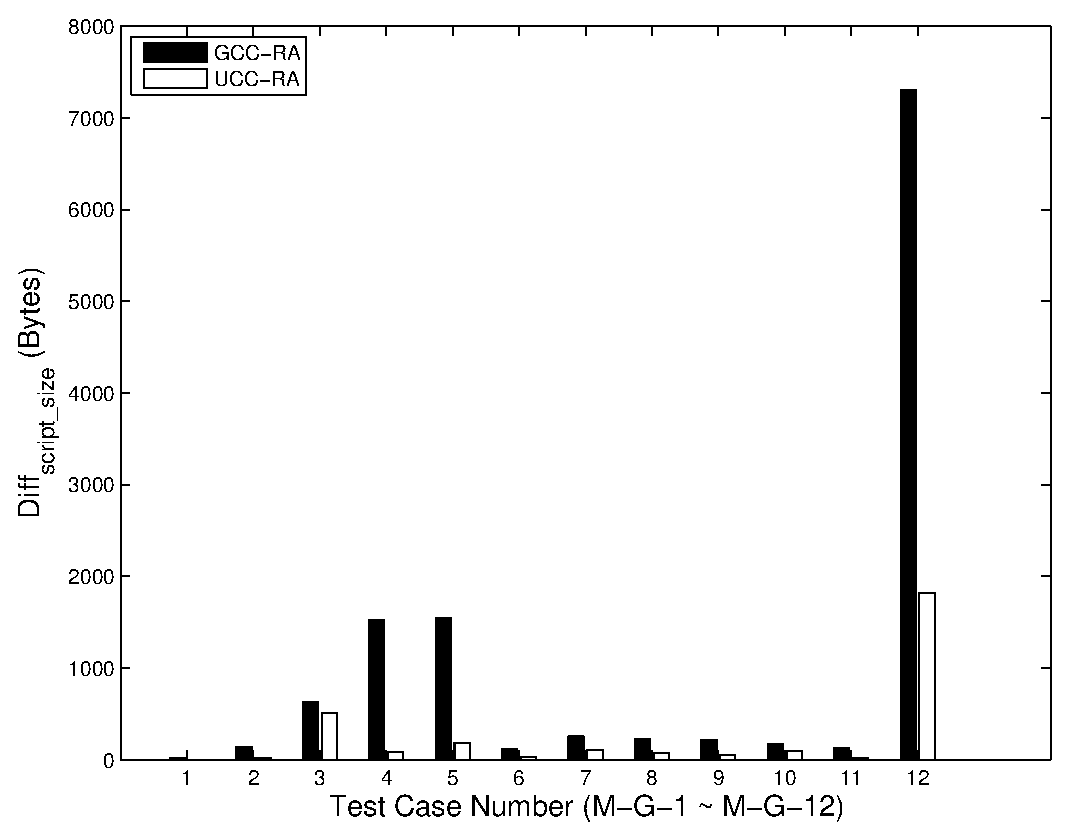
\includegraphics[scale=0.6]{figures/upd.eps}
\caption{The generation script size comparison between UCC-RA and GCC-RA.}
\label{fexp.upd}
\end{figure}

Figure \ref{fexp.upd} shows the results, in $\textit{Diff}_{script\_size}$, for update
test cases M-G-1 $\sim$ M-G-12.  As I can see, UCC-RA greatly reduces the code
difference as it effectively localizes the code changes --- the
majority of the code can be kept the same.  On the contrary, GCC-RA
may generate only local changes (test case M-G-1), but may also propagate local
changes to a much larger range (test case M-G-4).

I then studied the two large changes. Test case 12 introduces
several new functions most of which are small {\em inline}
functions. They disturb the register selection in a large function and
introduce significant number of differences, which are seen when using
GCC-RA. Fortunately, those differences are minimized in UCC-RA.
Test case M-G-13 represents another type of large
changes, the application {\tt CntToLeds} is quite different from
{\tt CntToRfms}.  The former has 828 instructions while the latter has
4351 instructions. It is an expensive update since all new instructions
and functions have to be disseminated across the network. There is
some code similarity due to the fact that applications in the same
TinyOS environment follow a generic structure.  GCC-RA can reuse 422
instructions and need to update 3929 instructions. UCC-RA can reuse 63
more instructions, which represents an increase of 15\% from GCC-RA,
and accounts for about 7.6\% of the old code ({\tt CntToLeds}).

\subsubsection{The generated code quality}
Next, I compared the code quality resulting from different
algorithms. The code quality is quantified using $\textit{Diff}_{cycle}$, the
changes in execution cycles between the old and new version of the
binary. This metric also indicates the slowdown in execution time
after applying update-conscious compilation.

\begin{figure}[htbp]
\centering
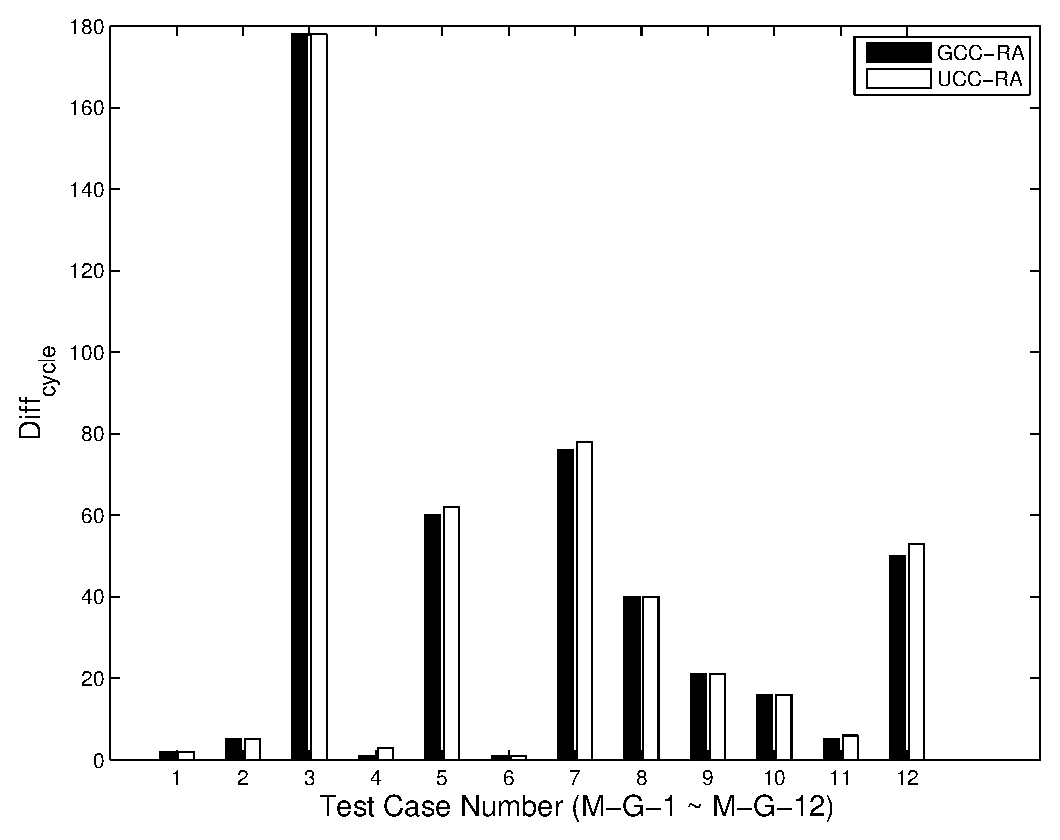
\includegraphics[scale=0.6]{figures/prof.eps}
\caption{The generated code quality between UCC-RA and GCC-RA (single run).}
\label{fexp.perf}
\end{figure}

Figure \ref{fexp.perf} shows the results for test case M-G-1 $\sim$ M-G-12. In
most of these cases, UCC-RA and GCC-RA have the same $\textit{Diff}_{cycle}$,
i.e. they have the same code quality. This is because both of them can
find free registers to use, and no extra spill code need to be
generated. Thus, register conflicts are small.  In some cases, e.g.,
test case M-G-12, UCC-RA inserts three {\tt mov} instructions since by
doing so, it can save 406 instruction updates and achieve overall
energy efficiency.

The slowdown from applying UCC-RA is negligible in nearly
all cases. For example, the three cycles introduced by UCC-RA in test
case M-G-12 accounts for less than 0.01\% of 244K cycles --- the total
number of cycles per single run for the application {\tt CntToRfm}. We
study its energy consumption over a long period after many
invocations, in the next section.

For test case M-G-13, UCC-RA only uses the preferred register tag as hint
when selecting registers. It has the same code quality as the one
generated by GCC-RA.

\subsubsection{The energy savings}
%To study the energy consumption in more detail, we conducted the
%experiment to compare the energy consumption using the above two
%register allocation algorithms.
The energy savings per update are calculated as follows. I first
compute $\textit{Diff}_{energy}$ (defined below), the energy consumption
difference (per single run) before and after the code update. It
incorporates the energy consumed in both data transmission and
instruction execution. Second, I compute the energy savings per
update for GCC-RA and UCC-RA respectively.

\begin{small}
\begin{eqnarray}
\lefteqn{\textit{Diff}_{energy} =}  \nonumber \\
& (\textit{Diff}_{script\_size} \times E_{trans} + \textit{Diff}_{cycle} \times E_{exe} \times Cnt) \\
\lefteqn{Energy Savings =} \nonumber \\
& Diff_{energy}^{GCC-RA} - Diff_{energy}^{UCC-RA}
\end{eqnarray}
\end{small}

\noindent
where $Cnt$ is the total number of times that the code may be executed
before it retires. A code retires when either it is overwritten by
a later update or the sensor node has consumed all its battery energy
and dies.

Figure \ref{fexp.energy} plots the the energy savings of UCC-RA over
GCC-RA as a function of $Cnt$, which is projected from the execution
profiles and the code update frequency. Code fragments that reside in
a loop, or retire after a long time, have larger $Cnt$s than
others. From the figure, I can see that when UCC-RA and GCC-RA
generate the same quality code (same \textit{Diff$_{cycle}$}, such as for test
case 1), the energy savings are independent of $Cnt$. The savings
mainly come from the reduced transmission energy. The larger number
of instructions I reduce from GCC-RA, the less data I need to
transmit, and the more savings I gain from UCC-RA.

When the code generated from UCC-RA runs slightly slower than that from GCC-RA (e.g., test case M-G-12), extra energy will be consumed in instruction execution. This can diminish the transmission energy savings when the code is executed very frequently. Therefore, UCC-RA adaptively inserts {\tt mov} instructions according to execution profiles and update frequency. A large $Cnt$ would disable the insertion such that UCC-RA and GCC-RA have the same energy consumption in the worst case. For example, UCC-RA falls back to take the GCC-RA's decision when the modified in code test case 12 is projected to execute more than 10$^7$ times.
%because of the diminishing energy gain.

\begin{figure}[htbp]
\centering
\includegraphics[scale=0.3]{figures/energy.eps}
\caption{The energy savings per update with different code execution frequency.}
\label{fexp.energy}
\end{figure}

\subsubsection{The problem complexity and compilation time}
For a given program, automatically generated general purpose software update
benchmarks are used to evaluate the ILP problem
complexity which is affected by the number of constrains and the number of
decision variables and the compilation time spent solving the ILP problem.

Since the ILP problem is more complex to solve when the number of
instructions and variables increase, I discuss the problem complexity
in this section. Figure~\ref{fexp.inst.con} plots the number of
constraints as a function of instruction number. I can see that the
number of constraints increases almost linearly with the number of IR
instructions. I plot the number of iterations that the LP\_solve
\cite{lpsolve} requires as a function of (the number of variables
$\times$ the number of IR instructions) in Figure~\ref{fexp.iter.con}.
\begin{figure}[htbp]
\centering
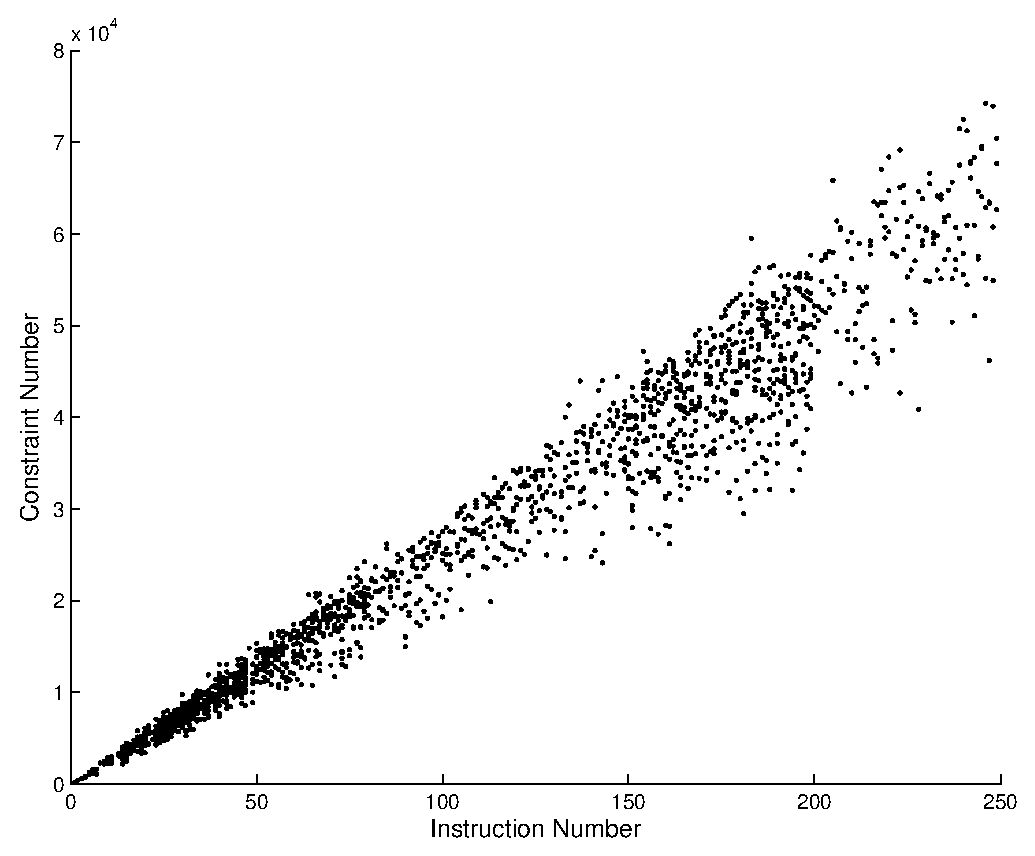
\includegraphics[width=4in]{figures/inst-cons.eps}
\caption{The number of constraints as a function of number
of IR instruction.}
\label{fexp.inst.con}
\end{figure}
\begin{figure}[htbp]
\centering
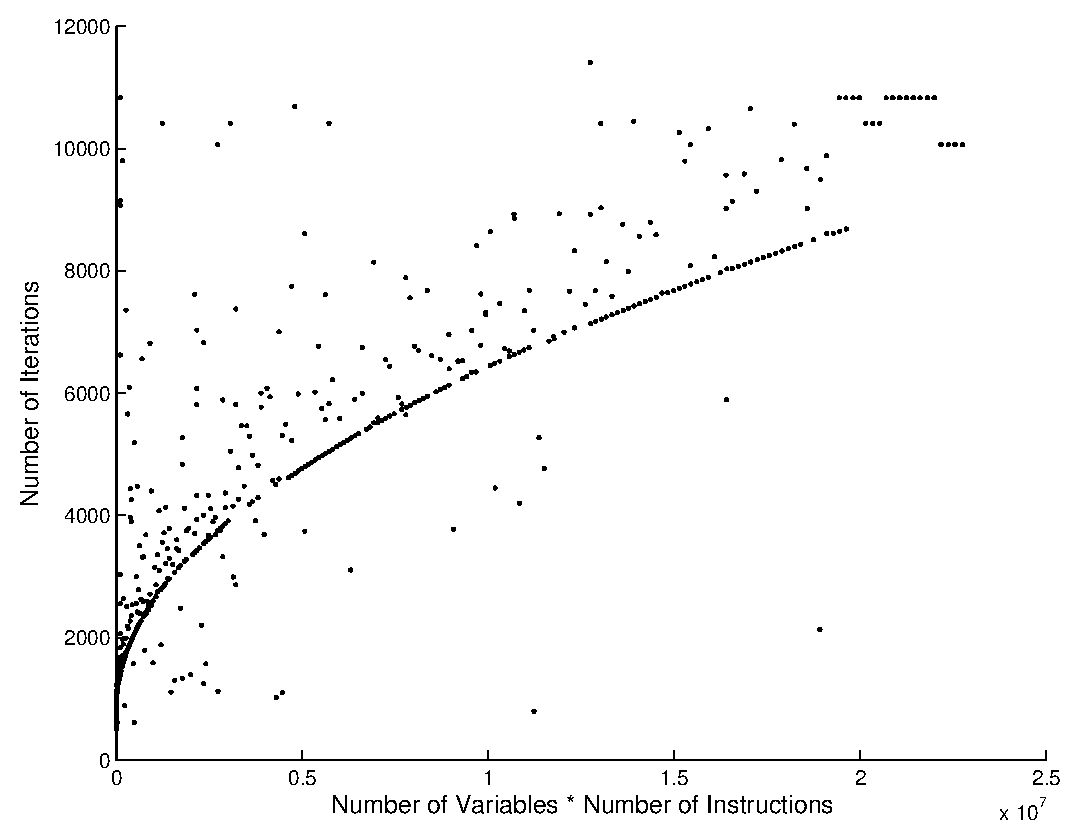
\includegraphics[width=4in]{figures/iter_linear.eps}
\caption{The number of iterations as a function of 
(the number of variables $\times$ the number of IR instructions).}
\label{fexp.iter.con}
\end{figure}

An interesting observation I found is that the preferred register tag
helps to improve the performance. Comparing to an ILP-based register
allocator which allocates register from scratch, the preferred
register tag is a hint to the solver and can reduce the number of
iterations that solver needs to try.  As an extreme case, I also
tested misleading preferred register tags, e.g., variables are
assigned to the preferred register tag randomly, I found the solver
may need 2 or 3 times more iterations to solve.

To see how fast the problem can be solved, I conducted timing
experiments on Intel Xeon 3.6GHz processor running Fedora Linux 2.4.21
kernel. The physical memory size is 2GB while in the experiments, the
largest observed memory usage is less than 256
MB. Figure~\ref{fexp.time.con} shows that the average time required to
solve one iteration increase about linearly with the problem
complexity.  It usually takes the solver less than 175 seconds to
allocate registers for a chunk of 250 IR instructions. As a
comparison, it takes GCC-RA less than one second to solve the same
problem. While UCC-RA is much slower than GCC-RA, it is not a
significant problem for WSNs due to the following reasons: (i) sensor
applications are small programs limited by the memory size of the
sensor node; (ii) UCC-RA is applied only to the identified {\em
changed} chunks instead of the complete functions or the whole
application; (iii) it is worthwhile to trade the compilation time at
the server side, where both energy and computation power are abundant,
for the energy savings on sensor nodes where resources are highly
constrained.
\begin{figure}[htbp]
\centering
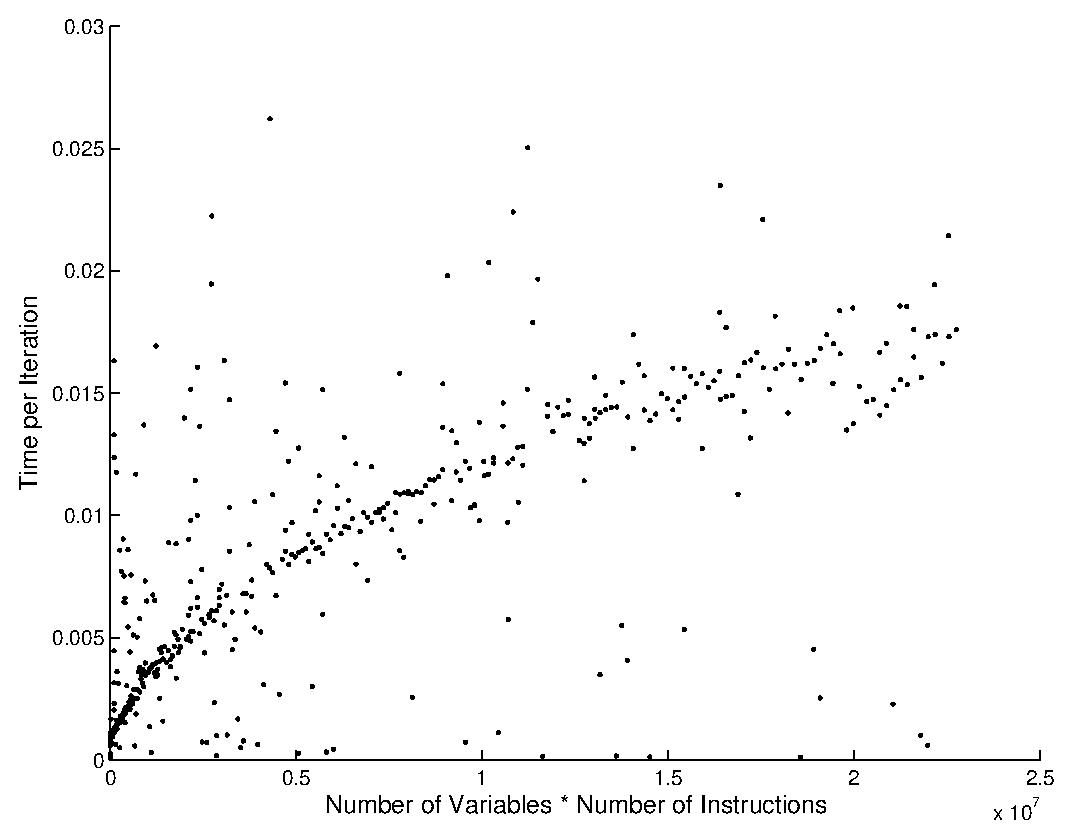
\includegraphics [width=4in]{figures/time_linear.eps}
\caption{The time to solve one iteration as a function of 
(the number of variables $\times$ the number of IR instructions).}
\label{fexp.time.con}
\end{figure}


I also performed experiments on testing whether approximating the
original non-linear integer programming problem with a linear problem
degraded the final results. I observed the same allocation decisions
for all the test cases with or without the approximation. The only
difference is that solving non-linear problems is orders of
magnitude slower than a linear problem.




\subsection{General purpose software update pre-dissemination 2}\label{exper-da}

In order to compare the performance of the proposed update-conscious compilation data
allocation scheme (UCC-DA) with GCC-DA, I used the manual generated general purpose 
benchmarks (M-G-14 $\sim$ M-G-19) list in
Figure~\ref{fbench.chg1} to generate the binary images and further the patch scripts.

The tradeoff of UCC-DA is between the stack size and the generate script size.
Keeping more local variables in the same location as the previous version reduces
the update script size. However, it may increase the stack size because when variables
are removed, the memory holes will not be filled because we want to 
keep the data allocation similarity. Thus, in the experiments, I evaluated both the
generated script size and the worst case stack usage using different data allocation
algorithms.

\subsubsection{Settings}

I used {\tt ncc}, the NesC compiler
included in TinyOS release, and {\tt avr-gcc}, the GNU C compiler
(GCC) re-targeted for AMTEL AVR micro controllers to get the baseline binary.

The generated binary is compared with the older version to generate
the update script. I compared the generated script size between GCC-DA
and UCC-DA.The wasted space threshold $SpaceT$ is set to 5 Bytes for the experiments.


Then, I used {\tt tos-ramsize}~\cite{ramsize}, the tool included in TinyOS release, to
generate the worst case stack size of the binary generated using
different data allocation schemes.

I used the TinyOS applications as my benchmarks. The simple applications
such as Blink, CntToRfms and CntToLeds, do not use many local variables,
because there is very little computation involved.
Thus, I chose the Advanced Encryption Standard (AES) application~\cite{aes} as the benchmark. 
It takes several steps to encrypt or decrypt the given data and in each step it does
some relatively complicated computation to get a temporary result and feeds that
to the next step. For example, in the  {\tt ShiftRow} step, it  
cyclically shifts the bytes in each row by a certain offset. 
Local variables are heavily involved here to store the temporary results.

The update benchmarks are created based on the AES application, 
shown in Figure~{fbench.chg1} M-G-14 $\sim$ M-G-19.
The medium size update includes code update that add or remove multiple
local variables in a single function. The large size update includes code update
that add or remove multiple local variables in multiple functions.


\subsubsection{The generated script size}

I first used UCC-DA and GCC-DA to generate the new binary, compared the
new binary with old one to generate the update script.
The script size comparison is shown in Figure~ref{da-upd}.
I set the wasted space threshold $SpaceT$ to be 5 Bytes for the experiments.

\begin{figure}[htbp]
\centering
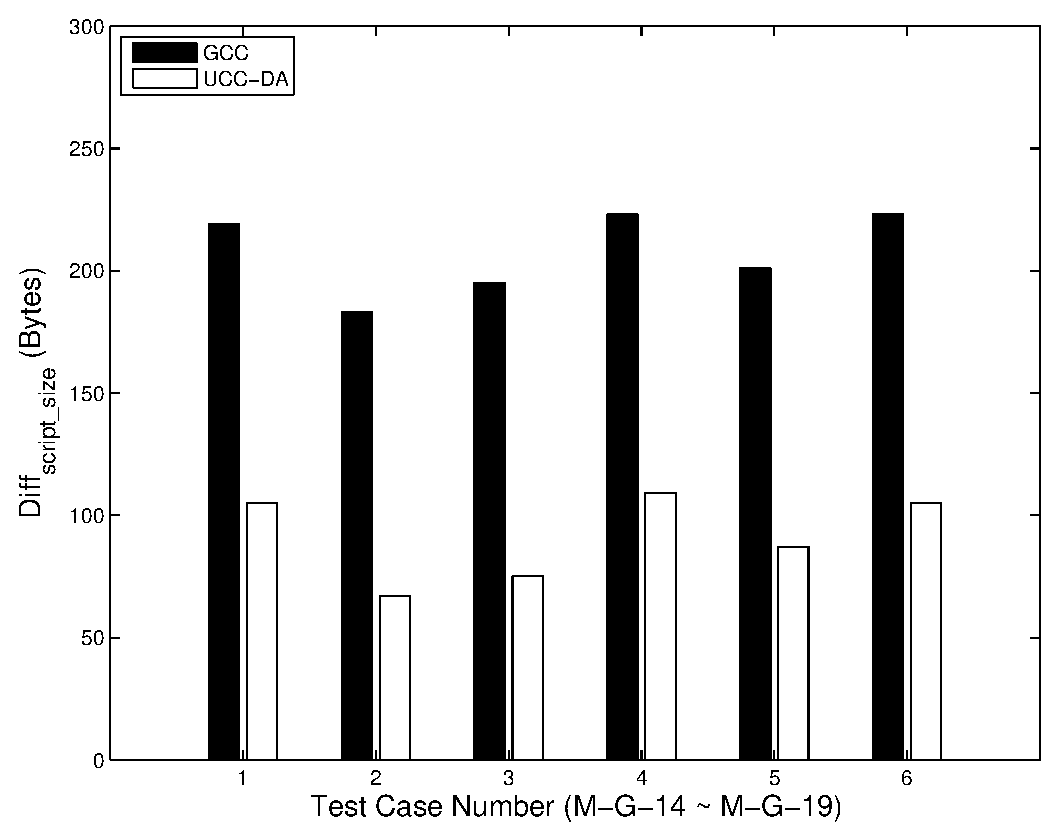
\includegraphics[scale=0.6]{./figures/da-upd.eps}
\caption{Script size comparison between GCC-DA and UCC-DA (general purpose applications).}
\label{da-upd}
\vspace{-0.1in}
\end{figure}

Using UCC-DA, the script size can be reduced by 56\% on average.
New variables are always allocated at the top of the stack no matter where they are
declared, so that the unchanged variables that are declared after these new variables
do not have to be reallocated.
For the deleted variables, the memory hole will be left unfilled, if the total wasted memory size
 is smaller than the threshold $Space_T$. Otherwise, the variable are selected
 to the fill up the holes based on the factor that is presented in ~\ref{factor}.
 Under the given threshold, the UCC-DA algorithm keeps most of the unchanged variables
in their original memory location, so that it minimizes the update to the memory access instructions
that access those variables.

\subsubsection{The wasted memory space}

The UCC-DA algorithm trades the memory space for the script size reduction. Keeping
the unchanged variables in place may cause memory holes if some variables are removed.
Thus, it may cause some memory waste and result in a larger worst-case stack size.
Figure~\ref{da-stack} compares the worst-case stack size of the binaries generated
by different data allocation algorithms.

\begin{figure}[htbp]
\centering
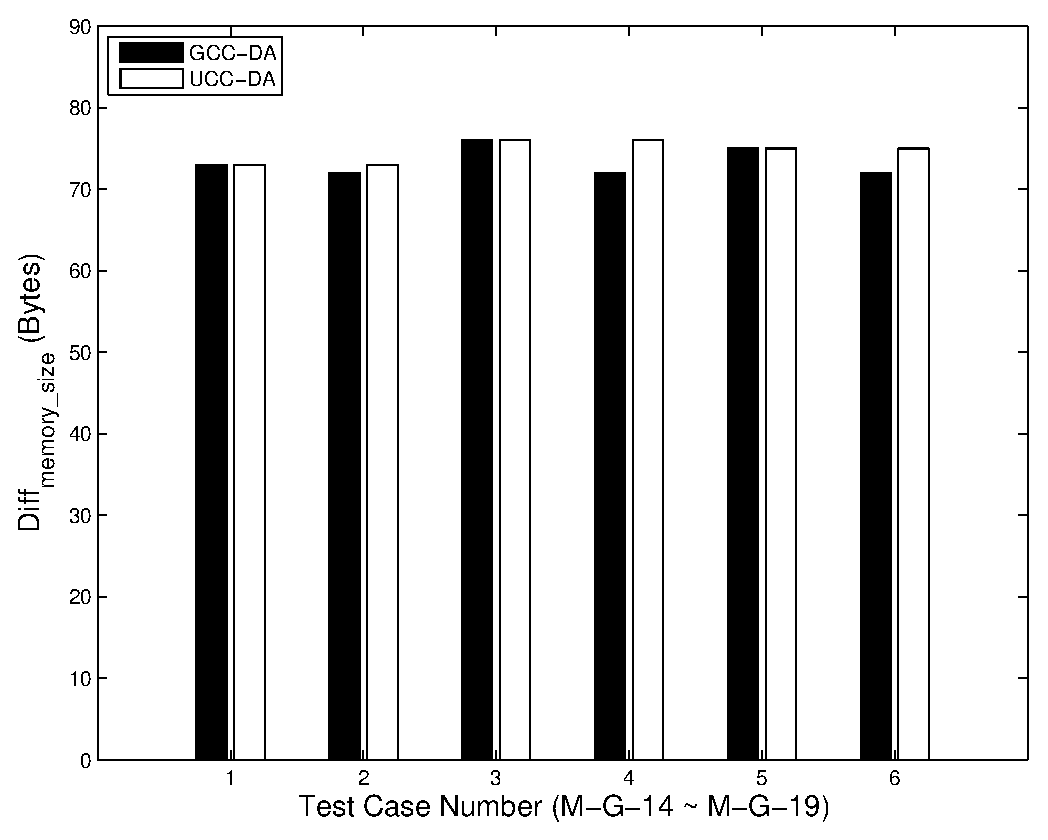
\includegraphics[scale=0.6]{./figures/stacksize.eps}
\caption{Worst-case stack size comparison between GCC-DA and UCC-DA (general purpose applications).}
\label{da-stack}
\vspace{-0.1in}
\end{figure}

From the experiment results, using UCC-DA only increases the memory usage by 1.9\% on average,
yet reduces the script size by 56\%.
This is because only when the memory space taken by the removed variables is larger than
the memory space needed by the inserted variables, the memory space may be wasted.
In real life, the most common reasons of code updates are adding new features or fixing existing bugs.
Changing existing code and adding new code are more likely to happen instead of removing 
existing code.

\subsubsection{Tradeoff between the wasted space and the instruction updates}

Shown in Figure~\ref{da-upd}, having the wasted space threshold $SpaceT$ set to be 5 Bytes gives 56\% script 
size deduction. Reducing this threshold may increase the script size, because more variables will
need to be moved to fill up the memory holes in order to meet this restriction.

Figure~\ref{da-tradeoff} shows such tradeoff.  I counted the number of instructions that need
to be updated due to data reallocation using GCC-DA.
Then, I compared that with the number of instructions that need to be updated due
to data allocation using UCC-DA, to compute the saved update \%.
With high wasted spaces threshold, the saved update \% is higher. 
Vice versa.

\begin{figure}[htbp]
\centering
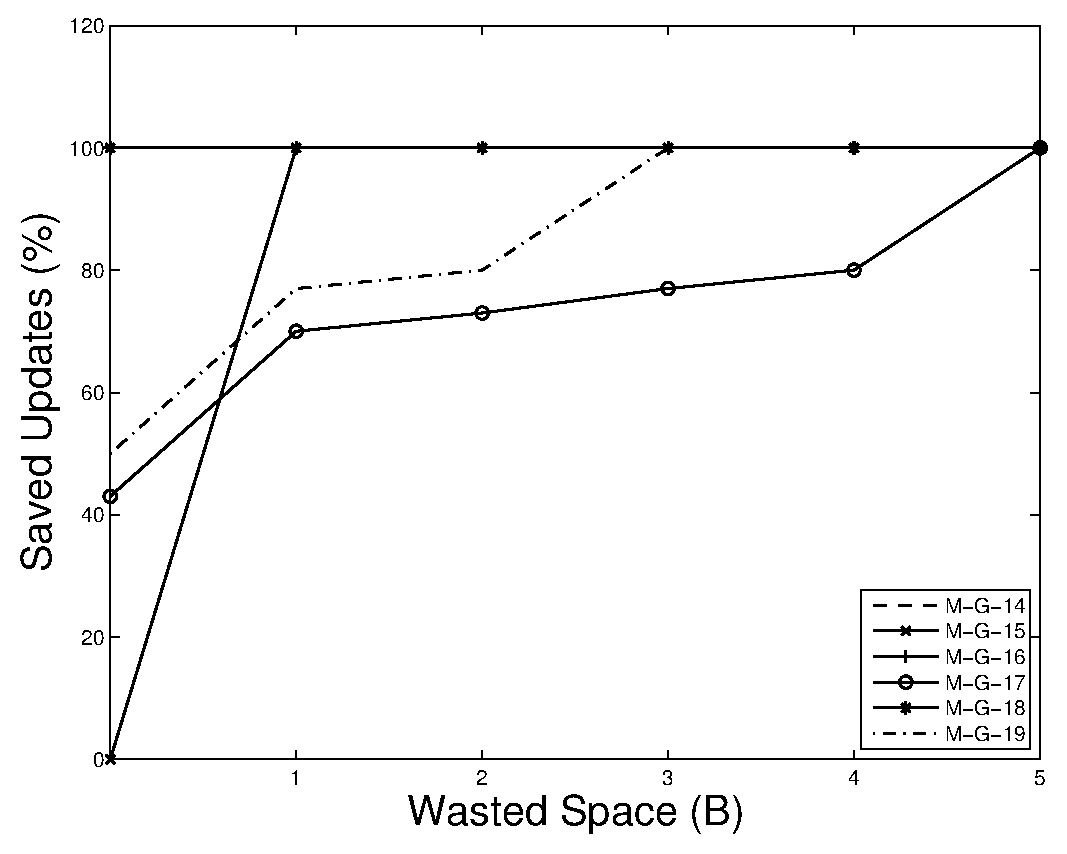
\includegraphics[scale=0.6]{./figures/spacetradeoff.eps}
\caption{Tradeoff between the worst-case stack size and the instruction updates.}
\label{da-tradeoff}
\vspace{-0.1in}
\end{figure}

From figure~\ref{da-tradeoff}, we can also see that the wasted space does not have to be high to
tolerant the instruction updates caused by data reallocation.
The worst-case stack size of the AES application is 67 Bytes. A 5 Byte memory waste
is large enough to tolerant all instruction updates caused by data reallocation, in the given
test cases.

An interesting observation is that even setting the threshold $SpaceT$ to be 0 Bytes can 
give some improvement, compared to the GCC-DA scheme. 
For example, test case M-G-14, M-G-16, and M-G-18 achieve 100\% update deduction
even when the threshold is set to 0 Byte.
This is happens when the memory space occupied by the deleted variables is smaller
than the space occupied by the inserted variables. 
Without the update-conscious scheme, the variables are ordered by the declaration 
sequence on stack. This may cause address shift to those unchanged variables
that are declared after these new variables. However, using the update-conscious scheme,
the new variables are first used to fill up the memory holes, and the extra new variables always 
allocated on top to the unchanged ones. Thus, these
unchanged variables will not be reallocated, so that less instruction updates will be
caused.

\subsection{General purpose software update pre-dissemination 3}

The experimental results in ~\ref{exper-ra} and ~\ref{exper-da} show that
using the Update-conscious register allocation and data allocation individually
can reduce the update script sizes by 71\% and 56\% representatively.
However, the performance loss caused by the update-conscious compilation schemes 
is very small, i.e., increasing the number of instructions in each execution by 
4.7\% and RAM usage by 1.8\%.

Integrating both the UCC-RA and UCC-DA schemes should combine the benefits
caused by both algorithms and reduce the script size even more.
I implemented the integration algorithm proposed in ~\ref{integration} and
ran the integration algorithm on the manual cases M-G-14 $\sim$ M-G-19.
The maximum wasted space threshold is set to be 5 bytes. The generated 
script size comparison is shown in Figure~\ref{general-inte}.

\begin{figure}[htbp]
\centering
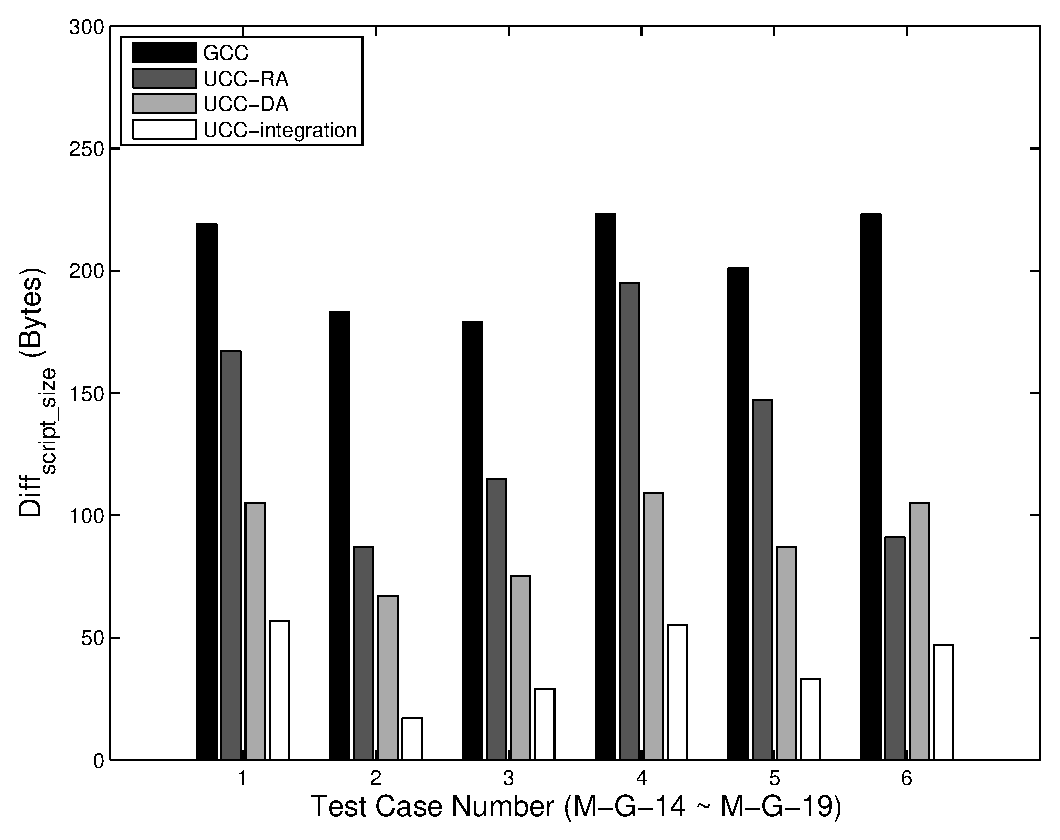
\includegraphics[scale=0.6]{./figures/inte-upd.eps}
\caption{The generated script size comparison between GCC and UCC integrated scheme.}
\label{general-inte}
\end{figure}

As shown in Figure~\ref{general-inte}, the integrated scheme produce the
smallest scripts compared to the individual UCC-RA and UCC-DA schemes. 


\subsection{DSP software update pre-dissemination}

In order to compare the performance of the proposed update-conscious compilation data
allocation scheme (GCC-DA) for DSP applications and the CSOA/CGOA schemes, I used the manual generated DSP
benchmarks (M-D-1 $\sim$ M-D-5) and the real DSP benchmarks (R-D-1 - R-D-3)
list in Figure~\ref{dsp-bench} and Figure~\ref{dsp-manual} to generate the binary image
and further the patch script using the proposed script primitives.
Then, I used the automatically generated DSP benchmarks to study the performance tradeoffs
for more general cases.

\subsubsection{Settings}
I have implemented the proposed update-conscious ICSOA/ICGOA algorithms. I chose the Lance Compiler\cite{lance} to convert the source code (C code) into intermediate representations (IRs) from which the access sequence and interference graph are extracted. I selected the DSPstone\cite{dspstone} benchmark suite that is widely used to measure the performance of DSP compilers. I adopted CSOA-Offsetstone\cite{offsetstone} as the baseline CSOA and implemented ICSOA on top of it. 
%
%I evaluated the impact as the number of variable interferences that are added by the code update, and whether these new interferences conflict with existing variable partitioning result. An interference conflict happens when two coalesced variables (in the old assignment) have overlapped live ranges and thus cannot be coalesced anymore.


\subsubsection{The generated script size}
\ \\


\textbf{Single offset assignment}
Figure \ref{update} compares the software update overhead for CSOA and ICSOA. I used three script formats to do the comparison.
\begin{itemize}
\itemsep 0pt
\item
{\it Simple code update script} that uses only the simple code primitives;
\item
{\it Advanced code update script} that uses all types of the code primitives;
\item
{\it Context-aware update script} that uses both code and data primitives.
\end{itemize}

Using the same script generator with ICSOA, the update script size can be reduced by 32\%.
This is because that the update-aware scheme follows the variable coalesces and offset assignment of the old code. The generated code has better code similarity to the old version in terms of both offset assignment and instruction addressing mode. In Test-Case M-D-1, the code update is very small such that the difference between the old and new offset assignments is not big. I did not see much benefit using ICSOA over CSOA. 

When comparing different script generators, I observed that  the advanced script generator produces a smaller script due to its usage of the {\it insert\_access} primitive. When there is no variable access insertion but contains removal or update in the code update, the two script generators produce the same script i.e. Test-Case M-D-4 and M-D-5.


The {\em context-aware} script generator produces smaller scripts when the code update is medium. Instead of sending individual instruction differences, it just sends out the data allocation differences, from which each node generates the new binary by itself i.e. Test-Case M-D-4 and M-D-5. I see a significant script size reduction by using this scheme. 
Adopting context-aware script tends to incur large complexity i.e. Test-Case M-D-1 and M-D-3 where I see a small script size increase due to the complexity to specify the offset assignment change. 
When the code has significant changes e.g. Test-Case R-D-3 introduces 32\% code changes, the old and new code segments are mixed such that the benefit from keeping the old data offset assignment diminishes.

\begin{figure}[htbp]
\centering
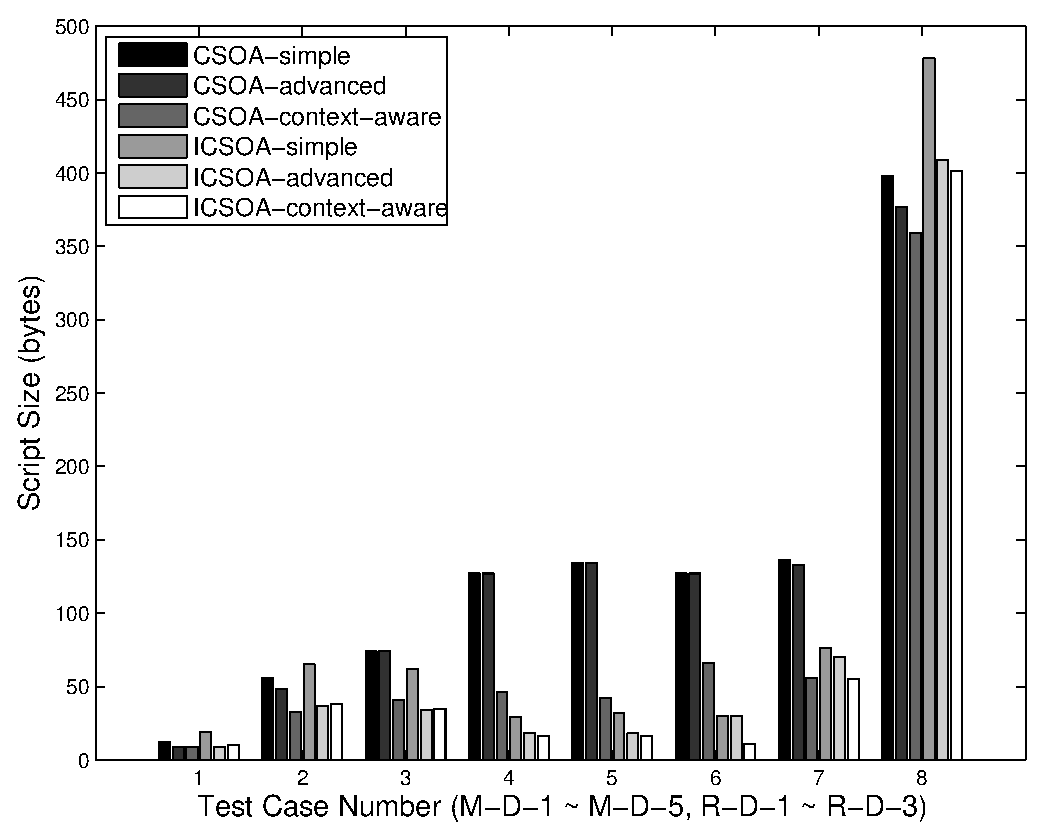
\includegraphics[scale=0.6]{./figures/update.eps}
\caption{Script size comparison between CSOA and ICSOA (Single address register).}
\label{update}
\vspace{-0.1in}
\end{figure}

\textbf{General offset assignment}
When there are multiple ARs, Figure \ref{update2} compares CGOA and ICGOA schemes with the different script generators. 

\begin{figure}[htbp]
\centering
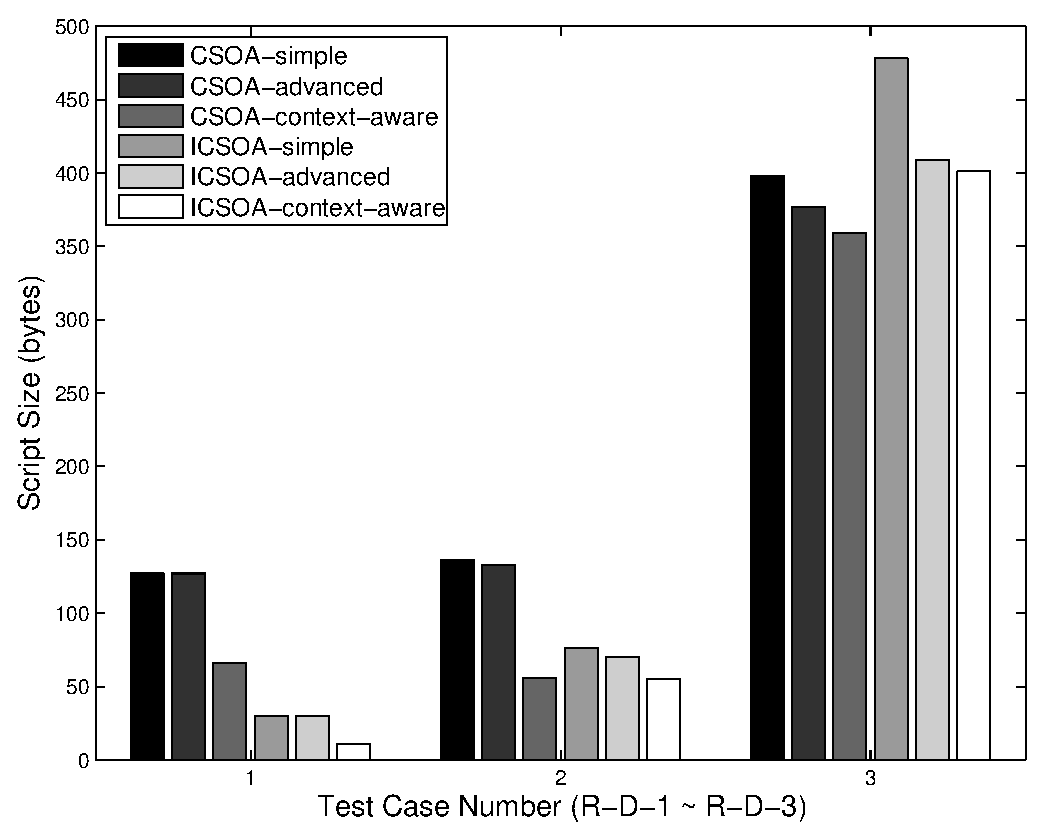
\includegraphics[scale=0.6]{./figures/update2.eps}
\caption{Script size comparison between CGOA and ICGOA (Double address register).}
\label{update2}
\vspace{-0.2in}
\end{figure}

When there are more ARs, recompiling the program results in large changes in both the variable
partition and offset assignment. For Test-Case 3, CGOA with context-aware script has larger size than that with simple script. This is because that the significant variable partition change and requires more primitives to specify the new offset layout. 

In conclusion, ICSOA/ICGOA is preferred when there are medium changes while recompilation is preferred when the change is small or big.

\subsubsection{The generated code quality}
In this paper I evaluated the static code quality i.e. the number of instructions in the new binary produced by CSOA and ICSOA schemes. An alternative approach is to evaluate the dynamic code quality i.e. the runtime instruction counts with given execution profiles. Although the latter provides more accurate evaluation, as I discussed in the introduction section, embedded mobile systems can periodically recharge the battery, so the execution overhead is less critical compared to its the communication overhead.

\textbf{Single offset assignment}
As shown in Figure \ref{exetotal}, ICSOA produces about the similar number of instructions as CSOA. On average, the binary generated by ICSOA is 10\% larger than the binary generated by CSOA. And for the worst test case, i.e. Test-Case 3, the binary generated by ICSOA is 23\% larger than CSOA. Because the ICSOA scheme incrementally does the data allocation based on the {\it coalesced access graph} of the old version, the old variable coalescing result is kept in the new version to improve code similarity. As a result, the code generated by ICSOA is not as efficient. 

\begin{figure}[htbp]
\begin{center}
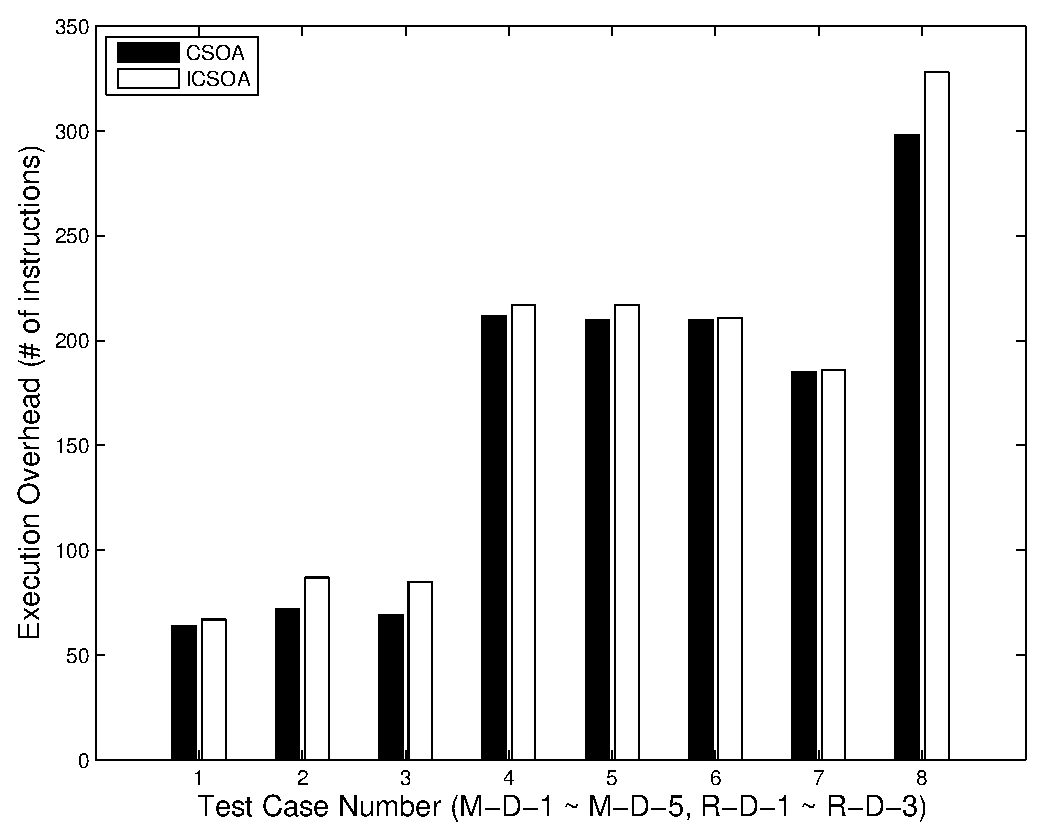
\includegraphics[width=4in]{./figures/exe.eps}
\caption{Code quality comparison between CSOA and ICSOA.}
\label{exetotal}
\end{center}
\vspace{-0.2in}
\end{figure}


To better understand the code quality difference between two approaches, Figure \ref{exebreakdown} shows the breakdown of the execution overhead. I separated the new code at the intermediate representation (IR) level into the changed and unchanged parts. I then create their mapping to the binary level code segments.


\begin{figure}[htdp]
\begin{small}

\begin{center}
\begin{tabular}{|p{0.5in}|p{0.2in}p{0.2in}p{0.2in}p{0.2in}|p{0.2in}p{0.2in}p{0.2in}p{0.2in}|}
\hline 
Test &\multicolumn{4}{c|}{CSOA} & \multicolumn{4}{c|}{ICSOA} \\
Case\# & T1 & T2 & T3 & T4 & T1 & T2 & T3 & T4\\
\hline \hline
M-D-1	&0	&7	&1	&0	&0	&7	&2	&0	\\
								
M-D-2	&1	&7	&9	&0	&0	&8	&12	&3	\\
									
M-D-3	&1	&7	&7	&0	&0	&10	&12	&6	\\
									
M-D-4	&4	&24	&0	&0	&0	&24	&2	&1	\\
									
M-D-5	&4	&22	&0	&0	&0	&24	&2	&1	\\

\hline

\end{tabular}
\end{center}
\caption{Execution overhead breakdown.}
\label{exebreakdown}
\end{small}
\vspace{-0.1in}
\end{figure}


Due to the change to offset assignment, the same IR instructions may be different in the old and new code. The change could be categorized into two types: (1) updating the addressing mode of the related binary instructions, such as the first memory access in Figure \ref{recomdiff}; (2) adding addressing mode change instructions. The first type update does not change the instruction number as no extra instruction is added,
but for the second type, one extra instruction is added per change. 

To study the code quality, I divide the overhead into four categories as follows. T1-T3 shows how efficient the offset assignment algorithm is; and T4 shows how the extra patch affects the final result.
\begin{itemize}
%\itemsep 0pt
\item T1: AR loading instructions removed from the old code;
\item T2: AR loading instructions inserted into the old code;
\item T3: AR loading instructions inserted into the new code;
\item T4: ALU instructions inserted into the new code.
\end{itemize}

Comparing columns T1 and T2 of both CSOA and ICSOA in Figure \ref{exebreakdown}, I found that CSOA generates less binary instructions for the unchanged IR part. It removes more AR loading instructions, and inserts less such instructions. For the new code part, CSOA generates less AR loading instructions. When performing complete recompilation, CSOA uses the new access sequences and variable interferences of the whole function, and thus can generate the better offset assignment.

Column T4 shows the number of ALU instructions generated by compiling the new assembly code.  Since ICSOA needs to add patch variables to remove the interferences due to overlapped live ranges, it adds several ``move'' instructions in the code, which causes more T4 type instructions.

\textbf{General offset assignment} For the test case M-D-3 that has the largest code quality difference, I increased the number of available ARs, and found that with more available ARs, the code quality difference is reduced, as shown in Figure \ref{exe_ar}. The extra instruction number drops from 20\% to 6\% when the address register number is increased from 1 to 4. 
This is because with more ARs, the variables are partitioned into smaller sets. The software update tends to create less new interference and needs fewer patch variables. Fewer interferences result in less overhead in ICSOA. 

\begin{figure}[htbp]
\begin{center}
\includegraphics[width=4in]{./figures/exe_ar.eps}
\caption{Code quality comparison with multiple ARs.}
\label{exe_ar}
\end{center}
\vspace{-0.2in}
\end{figure}

\subsubsection{The energy savings}
Compare the energy saving tradeoffs.

\subsubsection{Performance evaluation using automatically generated benchmarks}
I next inserted changes randomly into a file ({\em verify.c}) to study the robustness of my proposed scheme. The inserted code involves the use of both existing and new variables. The ratio of these two types is 1:1, and the sizes of the inserted/changed code range from 5\% to 60\% of the original code. Given an update percentage, I randomly generated 500 test cases and reported the average.

The script size comparison is shown in Figure \ref{upd_rand_bar}. For all three types of the script generation schemes, incremental compilation scheme reduces more of the
update script size and thus the software update transmission overhead. However, the results show that I achieved the maximum script size reduction when the update percentage is between 10\% and 40\%. This is because ICSOA benefits more when most of the update is caused by the data allocation changes rather than new/updated instruction operations. When the update percentage is too big, i.e. larger than 40\%, most changes are new or updated instructions. When the update percentage is too small, i.e. smaller than 20\%, the data allocation table is less likely to change even with recompilation. Thus, the benefits from ICSOA are limited.


\begin{figure}[htbp]
\begin{center}
\includegraphics[width=4in]{./figures/upd_rand_bar.eps}
\caption{Script size comparison between recompile and incremental-compile (scattered random new code insertion).}
\label{upd_rand_bar}
\end{center}
\vspace{-0.2in}
\end{figure}

The code quality is compared in Figure \ref{exe_rand_bar}. Larger code update percentage, i.e. over 40\%, has more live range extension of old variables, which produces more patch variables and instructions. Thus, the code produced by the recompilation scheme has a larger number of T4 type instructions; the code generated by the ICSOA scheme has a worse execution performance. 


\begin{figure}[htbp]
\begin{center}
\includegraphics[width=4in]{./figures/exe_rand_bar.eps}
\caption{Code quality comparison between recompile and incremental-compile (scattered random new code insertion).}
\label{exe_rand_bar}
\end{center}
\vspace{-0.2in}
\end{figure}


From Figure \ref{exe_rand_bar} and Figure \ref{upd_rand_bar}, I conclude that when the code update percentage is between 20\% and 40\%, using the update-conscious offset assignment scheme can save about 30\% of the transmission overhead, assuming that advanced script is used, with about 2\% extra instruction execution.


From the experimental results, I can also see that the simply using the code primitives works better with the incremental compilation scheme, and the context-aware scheme works better with the recompilation scheme.
This is because that the context-aware scheme trades updating individual instructions for setting up the auxiliary data structures and letting the sensors to construct these updates.
Thus, when I recompile the new version, a relatively large number of instructions are changed due to the data allocation differences, so the context-aware scheme can gain more benefit by saving those updates. 
On the other hand, when I use the incremental compilation technique, the saving is not great enough to balance the spending in setting up the data structures, therefore, just using the code primitives is more beneficial. 




\section{Patch dissemination}
\subsection{Settings}
I implemented MCP on the TinyOS~\cite{tinyos} platform. For comparison, I also implemented Melete~\cite{melete} and studied various network settings using TOSSIM~\cite{tossim}. 

I simulated mesh MA-WSNs of different sizes. I set the default spacing factor to 15 and model the lossy communication channel using the tool provided by TinyOS. There are four applications each of which is uniformly distributed across the network. In the default setting, 30\% of the sensors have application {\tt A} and there is a request from the sink to reprogram 20\% of the other sensors to run {\tt A}. MCP disseminates the code from in-network sources instead of the sink. 

\subsection{Message overhead}

\begin{figure}[htbp]
\centering
\includegraphics[width=4.2in]{figures/fsizes.eps}
\caption{Message overhead.}
\label{fmsg}
\end{figure}

Fig.~\ref{fmsg} shows the breakdown of the number of messages with different dissemination protocols. Without considering advertisement messages, Melete and Deluge have about the same message overhead, which was also reported in \cite{melete}. There are a large number of {\tt ADV} messages in Deluge, and a negligible number in Melete. The reason of such difference is Deluge depends heavily on incoming {\tt ADV} message, e.g., a sensor node only sends out new requests if it receives {\tt ADV} messages indicating its neighbors have more up-to-date data. Instead, in Melete, requesters receive the command from the sink code and then know the target application and its size. The requesters can proactively send out more requests after timeouts or receiving one complete page. The {\tt ADV} messages contribute to 37-40\% of the total message overhead in Deluge. 

My scheme takes a similar approach as Melete but requires some {\tt ADV} messages to update the AIT before, during and after the code switch. The {\tt ADV}'s overhead is low compared to the request and data transfer message overhead. On average my scheme reduces about 20\% of the message overhead from Melete. The main reason for this reduction is that Melete tends to have multiple responders within a small range and has a higher possibility of signal collision. MCP alleviates the problem by chosing one closeby source, which reduces the number of data packets in transmission.

\subsection{Completion time}

\begin{figure}[htbp]
\centering
\includegraphics[width=4.2in]{figures/ftime.eps}
\caption{Dissemination Time.}
\label{ftime}
\end{figure}

Fig.~\ref{ftime} compares the dissemination completion time of the different protocols. For the Deluge result, I record the time interval used by all requesters to complete the new code downloading. In practice, the Deluge protocol may still proceed to flood all sensors since it is not designed to update a subset of sensors. MCP requires less time to finish dissemination; on average it saves 45\% and 25\% over Deluge and Melete respectively.

\subsection{Sensitivity to Node Distribution}

\begin{figure}[htbp]
\centering
\includegraphics[width=4.2in]{figures/fdist1.eps}
\caption{Dissemination with Different Number of Sources and Requesters.}
\label{fsr}
\end{figure}

\begin{figure}[htbp]
\centering
\includegraphics[width=4.2in]{figures/fdist3.eps}
\caption{Dissemination with Uneven Source/Requester Node Distribution.}
\label{floc}
\end{figure}

Fig. \ref{fsr} illustrates message overhead with a different number of sources and requesters. I omit the dissemination time figure which exhibits similar results.
Along the X axis, (a,b) denotes that out of all the sensor nodes, a\% sources and b\% requesters are randomly selected in the field. I observed that the overhead tends to increase with more requesters and fewer sources. The difference is not significant.


Fig. \ref{floc} compares the message overhead when sources and requesters are distributed with location concentration. {\tt EvenD} denotes that all nodes are evenly distributed. {\tt CornerD} denotes that sources and requesters are distributed at the two diagonal corners of the rectangle field. {\tt SideD} denotes that sources and requesters are distributed along two sides of the field. From the figure, Melete has better performance than Deluge under even distribution. However, it generates significant conflicts and performs worse than Deluge when the nodes are unevenly deployed. MCP has consistently better results over Melete and Deluge. For the corner and side settings, MCP and Deluge are similar as almost all nodes are involved in the dissemination. 


\subsection{Sensitivity to Application Sizes}
Fig. \ref{fnumPage} shows message overhead with different application sizes. 
Due to the epidemic dissemination, Deluge exhibits approximately linear message overhead when
increasing the application size from 8 to 16 pages. Both Melete and MCP greatly reduce the communication overhead; however, they have slightly more than linear message overhead due to independent page requesting from requesters. MCP has a nearly constant message overhead reduction versus Melete, varying from 17.5\% for 8 pages to 18.1\% for 16 pages.

\begin{figure}[htbp]
\centering
\includegraphics[width=4.2in]{figures/fdist2.eps}
\caption{Dissemination with Different Number of Pages.}
\label{fnumPage}
\end{figure}


\subsection{Sensitivity to Cache Sizes}
Fig. \ref{fcache} summarizes message overhead of Melete and MCP with different cache sizes, i.e., the number of code pages that may be cached in memory. Here N=1 denotes that there is no caching. From the figure, MCP achieves significant communication overhead reduction when caching one or two future pages, and diminishing benefits when with larger cache sizes. The reason is that in MCP, a request message can preempt a working node (a source, a requester, or a forwarder) if that node works on a page with a larger page number and the page index difference is bigger than one. In this way, MCP prioritizes slow requesters such that they can keep up the pace with the nearby dissemination and take advantage of cached packets on the neighboring sensors.

\begin{figure}[htbp]
\centering
\includegraphics[width=4.2in]{figures/fcache.eps}
\caption{Dissemination with Different Cache Sizes.}
\label{fcache}
\vspace{-0.2in}
\end{figure}


\section{Case study}


\subsection{General purpose software update}
I used the real general purpose benchmarks (R-G-1 \~ R-G-6)
listed in Figure~\ref{fdeluge.src} to study the performance tradeoffs and
energy savings for real software update cases.
I used both GCC and UCC to get new binaries after each update, and then generate the update scripts according using update primitives described before. These scripts are distributed to the network using
the proposed MCP protocol and Deluge protocol to compare the network traffic and time savings.

\subsubsection{The generated script size}
Figure~\ref{fdeluge.data} shows the comparison results which include the number of script instructions per each type of primitive, and the final script size (bytes) for these two compilation techniques. In the case study, I did not add new instructions such that the performance is the same.

\begin{figure}[htbp]
\begin{center}
\begin{small}
\begin{tabular}{||p{0.5in}||p{0.38in}|p{0.15in} p{0.15in} p{0.2in} p{0.2in} p{0.15in}||
                           p{0.38in}|p{0.15in} p{0.15in} p{0.2in} p{0.2in} p{0.15in}||} \hline

Case \# & GCC Script Size (bytes) & \#A & \#R & \#P & \#C & \#L &  
          UCC Script Size (bytes) & \#A & \#R & \#P & \#C & \#L  \\ \hline \hline

R-G-1 &  \bf249 & 4&3&22&30&0    &\bf5  & 1&0&0&2&0  \\  \hline
R-G-2 &  \bf557 & 6&3&52&62&0    &\bf191& 8&3&1&4&0  \\  \hline
R-G-3 &  \bf447 & 2&1&39&43&0    &\bf12 &3&3&0&4&0   \\  \hline
R-G-4 &  \bf605 & 1&1& 4& 7&0    &\bf512 &6&0&1&8&0  \\  \hline
R-G-5 &  \bf277 & 0&4&31&36&0    &\bf35 &3&1&0&3&0  \\  \hline
R-G-6 &  \bf3981& 12&6&143&162&0 &\bf1069 &2&2&1&6&2 \\  \hline

\end{tabular}
\end{small}
\end{center}
\caption{Case study script size comparison (\#A: add primitive; \#R: remove primitive; \#P: replace primitive; \#C: copy primitive; \#L: clone primitive).}
\label{fdeluge.data}
\end{figure}

The average script size deduction for all the 6 test cases is 55\% comparing with GCC. This is because UCC reduces the instructions that need to be updated, thus the number of update primitives in the script is reduced. In addition, I found that when more instructions need to be updated, the code tends to be divided into smaller pieces, which results in more {\tt copy} primitives. For example in case R-G-3, UCC reduces the number of {\tt replace} primitives from 39 to 0, and {\tt copy} primitives from 43 to 4, which results in a 97\% script size deduction.

Notice that the {\tt clone} primitive is not frequently used in the script. This is because when the number of the instructions that can be ``cloned'' from the original code is not big enough, using {\tt replace} primitive is more efficient. For example, if there are {\tt N} instructions that can be ``cloned'' from the original code, which means that they are the same with the related instructions in the original code except for the register assignments, and a one-one mapping can be created between the register assignments in the two versions. The number of such register assignment mappings is {\tt M}. 
In such situation, I can use both {\tt clone} primitive and {\tt replace} primitive to represent the code updates. And the overhead of using each primitive is shown in the following equations.
\begin{small}
\begin{eqnarray}
Cost_{clone} = 5 + 2*M\\
Cost_{replace} = 1 + 2*N
\end{eqnarray}
\end{small}

\begin{small}
\begin{equation}
Cost_{clone} < Cost_{replace} \Rightarrow N-M > 2
\label{clonevsreplace}
\end{equation}
\end{small}

As shown in Equation \ref{clonevsreplace}, only when $N-M > 2$ is satisfied, I can gain more benefit by choosing the {\tt clone} primitive.


\subsubsection{Network traffic and transmission duration savings}

\textbf{MCP data needs to be added to this part.}

\begin{figure}[htp]
\centering
\includegraphics[width=4in]{figures/time.eps}
\caption{Duration time comparison.}
\label{fig:case.time}
\end{figure}

\begin{figure}[htp]
\centering
\includegraphics[width=4in]{figures/bytes.eps}
\caption{Data transmission comparison.}
\label{fig:case.bytes}
\end{figure}

Besides the script size comparison, I also used the software update protocol Deluge\cite{deluge} to disseminate the scripts to the wireless sensor network and measured the completion time and data size transmitted in the network. I used TOSSIM\cite{tossim}, the simulator provided by TINYOS\cite{tinyos} to disseminate these scripts over a 5x5 network. The scripts are injected to the sink node, and then propagated to the whole network.

I first compared the update duration time, which measures the time spent on routing these scripts in the network. It starts when the script injection to the sink node is finished, and ends when the whole network receives the scripts. The results are shown in Figure\ref{fig:case.time}. As larger scripts cost more time to propagate in the network, and UCC generates smaller scripts comparing with GCC, according to my experiment results, I can save 29\% dissemination time on average.

Then I compared the transmission overhead over the network between UCC and GCC.
I measured the size of the data transmitted over the network, which includes all three types of messages that are used by Deluge\cite{deluge}. Because the scripts are divided into fixed sized pages to transmit over the network, larger scripts produce more pages, which results in a high transmission overhead. In addition more pages tend to cause more communication conflicts over the network. On average UCC transmits 46\% less data during code dissemination.

\subsubsection{Energy saving analysis}
Present the energy saving achieved by each component.

%\subsection{Case study 2 -- UCC-General-DA + Script generation + Patch distribution}
%\begin{enumerate}
%	\item Benchmarks.
%	\item Collect the detailed script size comparison. Format like Figure~\ref{fdeluge.data}.
%	\item Collect the generated code performance comparison.
%	\item Transmission duration and traffic.
%\end{enumerate}


\subsection{DSP software update}
\subsubsection{The generated script size}
\subsubsection{Network traffic and transmission duration savings}
\subsubsection{Energy saving analysis}



\appendix
\bibliographystyle{abbrvnat}
\safebibliography{thesis1}

\end{document}
